\documentclass[11pt,reqno]{amsart}

\usepackage[margin=1in]{geometry}
\usepackage{amsmath,amssymb,amsthm,mathtools}
\usepackage{booktabs,array,multirow}
\usepackage{enumitem}
\usepackage{tikz}
\usetikzlibrary{calc,positioning,arrows.meta,decorations.pathreplacing,shapes.geometric}
\usepackage[colorlinks=true,linkcolor=blue!60!black,citecolor=green!45!black,urlcolor=blue!60!black]{hyperref}

\theoremstyle{plain}
\newtheorem{theorem}{Theorem}[section]
\newtheorem{lemma}[theorem]{Lemma}
\newtheorem{proposition}[theorem]{Proposition}
\newtheorem{corollary}[theorem]{Corollary}

\theoremstyle{definition}
\newtheorem{definition}[theorem]{Definition}
\newtheorem{construction}[theorem]{Construction}

\theoremstyle{remark}
\newtheorem{remark}[theorem]{Remark}

\newcommand{\ch}{\mathrm{ch}}
\newcommand{\chz}{\mathrm{ch}_0}
\newcommand{\chf}{\mathrm{ch}_{\mathrm{fin}}}
\newcommand{\Ffrz}{\mathcal{F}_{\mathrm{frz}}}
\newcommand{\Vge}{V_{\ge 4}}
\newcommand{\capf}{\mathrm{cap}}
\newcommand{\EG}{\text{Erd\H{o}s--Gy\'arf\'as}}
\emergencystretch=1.5em
\DeclareRobustCommand{\_}{\ifmmode\text{\textunderscore}\else\textunderscore\allowbreak\fi}

\title[Dyadic Cycles in Planar Graphs]{%
Every Cubic Planar Graph Contains $C_4, C_8, C_{16},$ or $C_{32}$:\\
Arbitrary Connectivity, Planar Claw-Free $C_{64}$,\\
and General Planar $C_{16}$ Theorems}

\author{Seth Rehwaldt}
\date{\today}

\begin{document}

\begin{abstract}
The \EG{} conjecture (1995) asserts that every finite graph with minimum degree at least $3$ contains a simple cycle whose length is a power of two. For $3$-connected cubic planar graphs, Heckman and Krakovski (2013) proved the existence of a power-of-two cycle of cycle length at most $128$; for planar induced claw-free graphs of minimum degree at least $3$, Daniel and Shauger (2001) proved the existence of a power-of-two cycle.

We establish four main theorems for finite nonempty simple planar graphs of \emph{arbitrary connectivity} (permitting disconnected graphs, bridges, cut-vertices, and $2$-cuts):
\begin{enumerate}[label=(\arabic*),leftmargin=2.2em]
  \item \textbf{All Cubic Planar Graphs (Sharp $C_{32}$):} Every finite nonempty simple cubic planar graph contains a simple cycle in $\{C_4, C_8, C_{16}, C_{32}\}$. This drops $3$-connectivity from Heckman--Krakovski and improves the cutoff fourfold from $128$ to the sharp threshold $32$, matching Exoo's $m \ge 5$ lower bound ($G_{420}$) and witnessed by an elementary $168$-vertex $6$-face-free $3$-connected cubic planar graph $G_{168} = C_{24} * [T_1 + P + T_2]$ with no $C_4, C_8, C_{16}$.
  \item \textbf{All Planar Induced Claw-Free Graphs (Explicit $C_{64}$):} Every finite nonempty simple planar induced claw-free (induced $K_{1,3}$-free) graph with $\delta(G) \ge 3$ contains a simple cycle in $\{C_4, C_8, C_{16}, C_{32}, C_{64}\}$, via planar bowtie-splitting and a universal cubic-to-claw-free transfer theorem applied to~(1).
  \item \textbf{General Planar $\delta \ge 3$ $C_{16}$ Trilogy (Arbitrary $\Delta$):} Every finite nonempty simple planar graph with $\delta(G) \ge 3$ that is $C_3$-free, $C_5$-free, or $C_6$-free contains a simple cycle in $\{C_4, C_8, C_{16}\}$. Each part is sharp, witnessed by the truncated icosahedron $C_{60}$, the truncated dodecahedron $TD_{60}$, and their $119$-vertex $\Delta = 6$ planar $1$-sums.
  \item \textbf{Alternating-$C_6$ Planar Degree-Density Bound:} Every finite nonempty simple planar graph with $\delta(G) \ge 3$, independent high-degree set $V_{\ge 4}$, and no $C_4, C_8$ satisfies $16 h + 4 \varepsilon \le 5(n - 2) + 4 \tau_6$, where $h = |V_{\ge 4}|$, $\varepsilon = \sum_{v \in V_{\ge 4}}(d(v) - 4)$, and $\tau_6$ is the $6$-cycle edge-transversal number of the mixed bipartite subgraph $G[V_{\ge 4}, V_3]$. In particular, when $C_6$-free, $|V_3| \ge \lceil(11n+10)/16\rceil > 2n/3$ for all $n \ge 7$, improving the $2/3$ density benchmark by $1/48$.
\end{enumerate}
Our verification artifact separates four transparent layers: (i)~core discrete algebraic, discharging, Bellman--Ford/DP soundness, and density lemmas proved in the pure Lean~4 kernel (\texttt{v4.36.0}, zero \texttt{sorry}, zero custom axioms, zero \texttt{native\_decide}); (ii)~proof-carrying Lean~4 certificates for packed dual potentials, DP/BWD upper bounds, $6{,}772$ strict-schema explicit simple dyadic-cycle patch entries (counted with multiplicity across certificate groups), and cellular-rotation sharpness witnesses; (iii)~standalone zero-float standard-library Python replay (\texttt{cert/verify\_planar\_eg.py}) of all underlying finite searches and uncollapsed DPs, paired with a runnable zero-float parity and weighted state-collapse verifier (\texttt{cert/verify\_parity\_and\_dp.py}) checking all $12$ weighted DP simulations and literal Lean--Python--JSON parity; and (iv)~full topological and graph-theoretic proofs in this manuscript.
\end{abstract}

\maketitle

\tableofcontents

%% =============================================================================
\section{Introduction and Main Results}\label{sec:intro}
%% =============================================================================

Formulated by Erd\H{o}s and Gy\'arf\'as in 1995 and published by Erd\H{o}s in 1997~\cite{Erdos1997}, the \EG{} conjecture asserts that every finite graph with minimum degree at least $3$ contains a simple cycle of length $2^k$ for some integer $k \ge 2$. While the conjecture is now known to hold for graphs of sufficiently large average degree---following the order-dependent average-degree bound $\bar{d}(G) \ge e^{C \log^* n}$ of Sudakov and Verstra\"ete~\cite{SudakovVerstraete2008} and culminating in the constant average-degree theorem of Liu and Montgomery~\cite{LiuMontgomery2023}---the original sparse regime $\delta(G) \ge 3$ remains open even for general planar graphs.

Three lines of prior work directly anchor our results:
\begin{itemize}[leftmargin=1.8em]
  \item \textbf{Cubic planar graphs and sharpness:} Heckman and Krakovski~\cite{HeckmanKrakovski2013} proved that every $3$-connected cubic planar graph contains a simple cycle of length $2^m$ with $2 \le m \le 7$ (cycle length at most $128$), asking whether the upper bound $m \le 7$ could be reduced. Exoo~\cite{Exoo2014} responded by constructing a $420$-vertex $3$-connected cubic planar graph $G_{420}$ (derived from the truncated icosahedron $C_{60}$, Section~2 of~\cite{Exoo2014}) with no $C_4, C_8,$ or $C_{16}$, establishing $m \ge 5$ (cutoff at least $32$). Earlier, Markstr\"om~\cite{Markstrom2004} found a $24$-vertex $3$-connected cubic planar graph avoiding $C_4$ and $C_8$; Garcia~\cite{Garcia2026} recently certified minimum order $24$ for avoiding $\{C_4, C_8\}$ across all $\delta \ge 3$ graphs, matching Markstr\"om's $24$-vertex cubic planar example and the cubic threshold $f(3) = 24$.
  \item \textbf{Claw-free and planar claw-free graphs:} Shauger~\cite{Shauger1998} proved the conjecture for $K_{1,m}$-free graphs with $\delta(G) \ge m + 1$ (including claw-free graphs with $\delta \ge 4$), and Daniel and Shauger~\cite{DanielShauger2001} proved that every planar induced claw-free graph with $\delta(G) \ge 3$ contains a power-of-two cycle (see also~\cite{HeckmanKrakovski2013}).
  \item \textbf{Degree-density in minimal counterexamples:} Using Markstr\"om's~\cite{Markstrom2004} observation that any minimal counterexample to the \EG{} conjecture has an independent high-degree set $\Vge$ together with new structural results, Carr~\cite{Carr2026} proved $|V_3| \ge \frac{4}{7}|V|$; Ducoffe and Dumitru~\cite{DucoffeDumitru2026} sharpened this to $|V_3| > \frac{2}{3}|V|$ for minimal counterexamples generally.
\end{itemize}

Throughout this paper, all graphs are \emph{finite, nonempty ($V(G) \neq \emptyset$), and simple} (no loops or parallel edges), unless explicitly noted otherwise. We write $\delta(G)$ and $\Delta(G)$ for the minimum and maximum vertex degrees of $G$, $V_3(G) = \{v \in V(G) : d_G(v) = 3\}$, and $\Vge(G) = \{v \in V(G) : d_G(v) \ge 4\}$. A \emph{dyadic cycle} is a simple cycle $C_{2^k}$ of length $2^k$ with $k \ge 2$. A graph is \emph{claw-free} if it contains no \emph{induced} subgraph isomorphic to $K_{1,3}$. Theorems~\ref{thm:main1}--\ref{thm:main4} below (numbered Theorems~1.1--1.4 in this section) correspond respectively to Main Theorems~1--4 in the accompanying verification artifact.

\subsection{Statements of Main Theorems}\label{subsec:statements}

\begin{theorem}[Main Theorem 1 --- All Cubic Planar Graphs, Sharp $C_{32}$]\label{thm:main1}
Every finite nonempty simple cubic planar graph $G$ (of arbitrary connectivity) contains a simple cycle of length $4, 8, 16,$ or $32$.

Moreover, the threshold $32$ is sharp: there exists an explicit $168$-vertex $3$-connected simple cubic planar graph $G_{168} = C_{24} * [T_1 + P + T_2]$ containing a simple $C_{32}$ and no simple $C_4, C_8,$ or $C_{16}$.
\end{theorem}

Theorem~\ref{thm:main1} strengthens~\cite{HeckmanKrakovski2013} simultaneously in two orthogonal directions: it removes the $3$-connectivity hypothesis completely (covering disconnected graphs, bridged graphs, and $2$-edge-cut graphs via a frozen-edge cap discharging method) and sharpens the dyadic cutoff fourfold from $128$ to the exact optimum $32$, closing the $m \in \{5, 6, 7\}$ gap left between~\cite{HeckmanKrakovski2013} and Exoo's construction $G_{420}$~\cite{Exoo2014}. Alongside Exoo's $420$-vertex $C_{60}$-derived construction $G_{420}$~\cite{Exoo2014}, our smaller elementary $168$-vertex, $6$-face-free $G_{168} = C_{24} * [T_1 + P + T_2]$ supplies a sharpness witness fully kernel-verified in Lean~4.

\begin{theorem}[Main Theorem 2 --- All Planar Induced Claw-Free Graphs, Explicit $C_{64}$]\label{thm:main2}
Every finite nonempty simple planar induced claw-free (induced $K_{1,3}$-free) graph $G$ with $\delta(G) \ge 3$ (of arbitrary connectivity and arbitrary maximum degree $\Delta$) contains a simple cycle of length $4, 8, 16, 32,$ or $64$.
\end{theorem}

Theorem~\ref{thm:main2} gives an independent proof of the planar claw-free theorem of Daniel and Shauger~\cite{DanielShauger2001} with the explicit universal bound $64$. It follows directly from Theorem~\ref{thm:main1} combined with our \emph{Planar Bowtie-Splitting Lemma} and \emph{Universal Cubic-to-Claw-Free Transfer Theorem} (Section~\ref{sec:clawfree}).

\begin{theorem}[Main Theorem 3 --- General Planar $\delta \ge 3$ $C_{16}$ Trilogy]\label{thm:main3}
Let $G$ be a finite nonempty simple planar graph with $\delta(G) \ge 3$ (of arbitrary connectivity and arbitrary maximum degree $\Delta$). If $G$ is
\begin{enumerate}[label=(\alph*),leftmargin=2.2em]
  \item $C_3$-free (triangle-free),
  \item $C_5$-free (pentagon-free), or
  \item $C_6$-free (hexagon-free),
\end{enumerate}
then $G$ contains a simple cycle of length $4, 8,$ or $16$.

Moreover, every part is sharp at $C_{16}$ for both cubic and non-cubic planar graphs: the truncated icosahedron $C_{60}$ ($60$ vertices, cubic, no $C_3, C_4, C_8$) and its planar $1$-sum $C_{60} \cdot C_{60}$ ($119$ vertices, $\delta = 3$, $\Delta = 6$) witness sharpness for~(a); the truncated dodecahedron $TD_{60}$ ($60$ vertices, cubic, no $C_4, C_5, C_6, C_7, C_8, C_9$) and its planar $1$-sum $TD_{60} \cdot TD_{60}$ ($119$ vertices, $\delta = 3$, $\Delta = 6$) witness sharpness for both~(b) and~(c).
\end{theorem}

As an immediate corollary of Theorem~\ref{thm:main3}, any finite simple planar graph with $\delta(G) \ge 3$ avoiding $\{C_4, C_8, C_{16}\}$ must simultaneously contain triangles ($C_3$), pentagons ($C_5$), and hexagons ($C_6$).

\begin{theorem}[Main Theorem 4 --- Alternating-$C_6$ Planar Degree-Density Bound]\label{thm:main4}
Let $G$ be a finite nonempty simple planar graph on $n = |V(G)|$ vertices with $\delta(G) \ge 3$ such that $\Vge(G)$ is an independent set and $G$ contains no $C_4$ and no $C_8$. Set $h := |\Vge(G)|$, $\varepsilon := \sum_{v \in \Vge(G)} (d_G(v) - 4)$, and let $\tau_6$ denote the minimum cardinality of an edge set $T \subseteq E(Q)$ meeting every $6$-cycle in the mixed bipartite subgraph $Q := G[\Vge(G), V_3(G)]$. Then $n \ge 7$ and
\begin{equation}\label{eq:alt-c6-density}
  16 h + 4 \varepsilon \;\le\; 5(n - 2) + 4 \tau_6.
\end{equation}
In particular:
\begin{enumerate}[label=(\roman*),leftmargin=2.2em]
  \item If $G$ is $C_6$-free (so $\tau_6 = 0$), then
  \begin{equation}\label{eq:v3-density}
    |V_3(G)| \;\ge\; \left\lceil \frac{11 n + 10}{16} \right\rceil \;>\; \frac{2}{3} n
  \end{equation}
  for every $n \ge 7$, strictly surpassing the $2/3$ coefficient by $11/16 - 2/3 = 1/48$.
  \item Even when $6$-cycles are permitted, any such graph with $|V_3(G)| \le 2n/3$ must satisfy $\tau_6 \ge \lceil (n + 30)/12 + \varepsilon \rceil$ and therefore contains at least $\lceil \tau_6 / 6 \rceil$ pairwise edge-disjoint alternating $6$-cycles in $Q$.
\end{enumerate}
\end{theorem}

\subsection{Honest Verification and Formalization Summary}\label{subsec:honest-scope}

Our proofs combine traditional structural graph theory and topological embedding arguments with extensive finite discharging casework (boundary-weld quotients, noncrossing outer-rim partitions, cyclic dynamic programming, and exact rational Bellman--Ford dual potentials). To guarantee mathematical reliability without overstating the scope of machine formalization, we explicitly partition every claim across four transparent verification layers:
\begin{enumerate}[label=(\roman*),leftmargin=2.2em]
  \item \textbf{Proved in the Lean~4 kernel (\texttt{lean/PlanarEG/}, pure Lean~\texttt{v4.36.0}, zero Mathlib):} Core discrete simple-graph predicates, Euler discharging conservation on combinatorial \texttt{PlaneMap} structures, local cap degree/avoiding-lift lemmas, universal vertex-absorption inequalities, exact budget identities, exhaustive $F_{10}$ $5$-triangle score maximization ($252 \times 123$ bitmask pairs, $\max = 47/12 < 4$), Bellman--Ford/DP/BWD soundness theorems, bowtie-forest exclusion arithmetic and inductive forest bounds, and alternating-$C_6$ density algebra. All $106$ audited declarations in \texttt{AxiomCheck.lean} depend solely on Lean's standard axioms $\{\texttt{propext}, \texttt{Classical.choice}, \texttt{Quot.sound}\}$, with zero \texttt{sorry}, zero custom axioms, and zero \texttt{native\_decide}.
  \item \textbf{Lean~4 proof-carrying finite certificates:} Kernel-checked dual potentials for all clean/frozen Bellman--Ford and DP state-graphs; kernel-checked strict face-schema validity (\texttt{WeldSchemaValid}) and explicit simple dyadic cycles on all $6{,}772$ eliminated weld and outer-rim entries (counted with multiplicity across certificate groups: $114 + 5 + 1{,}327 + 520 = 1{,}966$ for Theorem~\ref{thm:main1}, where the $5$ cubic $R_{10}$ seals are part of the $520$ seals and reused in the $d=17$ check; and $1{,}260 + 3{,}501 + 45 = 4{,}806$ for Theorem~\ref{thm:main3}); and kernel-checked exact dart bijections, single cyclic vertex rotations, $3$-connectivity ($G_{168}$), forbidden-cycle exclusions, and explicit target cycles for $G_{168}$, $C_{60}$, and $TD_{60}$.
  \item \textbf{Standalone zero-float Python replay (\texttt{cert/verify\_planar\_eg.py}) and parity/simulation verifier (\texttt{cert/verify\_parity\_and\_dp.py}):} Pure-stdlib Python~3 scripts (both AST-guarded against floating-point literals and true division~\texttt{/}). First, \texttt{cert/verify\_planar\_eg.py} replays all underlying finite searches, boundary-weld and rim-quotient enumerations, $51$-chain BFS, conservative $d \in \{14,17,18\}$ enumerations, exact uncollapsed cyclic DPs, Bellman--Ford potentials, and $119$-vertex $1$-sum witnesses in ${\sim}21\,\mathrm{s}$ and ${\sim}43\,\mathrm{MiB}$ RSS. Second, \texttt{cert/verify\_parity\_and\_dp.py} directly verifies literal parity across Lean~4 data modules, \texttt{cert/witnesses/*.json}, and live Python replay across all $6{,}772$ weld/rim entries, confirms the Lemma~\ref{lem:weld-sound} boundary-regularity invariant across all $844/844$ production calls, verifies all $12$ weighted forward-simulation checks linking the uncollapsed $C_5$-free ($7$ degrees: $d \in \{9..14, 17\}$) and $C_6$-free ($5$ degrees: $d \in \{9, 11..14\}$) DPs to the packed Lean automata, and replays all supplemental manuscript subaudits in ${\sim}43\,\mathrm{s}$ and ${\sim}70\,\mathrm{MiB}$ RSS (Section~\ref{sec:verification}).
  \item \textbf{Proved in this manuscript:} Topological spherical embeddings, Jordan curve arguments, Euler's formula with bridges/cut-vertices/components, Minimal $2$-Edge-Bond Cap and Universal $2$-Vertex-Cut Cap reductions, edge-minimality $\Vge$-independence, charge-conserving discharging rules by full configuration, graph-to-token maps and transition/flag derivations, completeness of hereditary boundary-weld and noncrossing outer-rim enumerations, conservative enumeration start/symmetry/shift/splice soundness, bowtie-forest/planar-skeleton/cycle-lift constructions, mixed bipartite $Q$/transversal/forest-Euler proofs for Theorem~\ref{thm:main4}, and planar $1$-sum gluing for the $119$-vertex sharpness witnesses.
\end{enumerate}
The complete Lean~4 library, Python verifiers, JSON witnesses, and SHA-256 manifest are publicly archived at \url{https://github.com/lollipoll/erdos-gyarfas} (directory \texttt{paper1\_planar/}); a complete theorem-by-theorem four-column traceability matrix appears in Section~\ref{sec:verification} and in the repository \texttt{README.md}.

%% =============================================================================
\section{Preliminaries, Planar Embeddings, and Connectivity-Cap Reductions}\label{sec:prelim}
%% =============================================================================

\subsection{Spherical Embeddings, Rotation Systems, and Euler's Formula}\label{subsec:euler}

Let $G = (V, E)$ be a finite nonempty simple graph ($|V| \ge 1$). A \emph{planar embedding} (or \emph{plane graph}) is a drawing of $G$ on the $2$-sphere $S^2$ in which vertices map to distinct points and edges map to internally disjoint simple Jordan arcs connecting their endpoints. Every connected plane graph with at least one edge induces a \emph{combinatorial rotation system}: letting $D(G) = \{(u,v), (v,u) : uv \in E(G)\}$ be the set of $2|E|$ \emph{darts}, the embedding specifies at each vertex $v \in V$ a single cyclic permutation $\sigma_v$ of the outgoing darts $\{(v,u) : uv \in E\}$ (clockwise cyclic order on $S^2$), together with the fixed-point-free dart-reversal involution $\alpha(u,v) = (v,u)$. The orbits of the face-traversal permutation $\phi := \sigma \circ \alpha$ are the \emph{facial boundary walks} of the embedding, bounding the connected components (\emph{faces}) of $S^2 \setminus G$ (with a bridge traversed once in each direction by the same facial walk; for a one-vertex component $K_1$, the unique face has facial walk length $0$).

For a plane graph $G$ with $c \ge 1$ connected components, $|V|$ vertices, $|E|$ edges, and $|F|$ faces, Euler's formula reads
\begin{equation}\label{eq:euler-general}
  |V| - |E| + |F| \;=\; 1 + c.
\end{equation}
Indeed, if $c = 1$ this is the standard connected spherical Euler formula $|V| - |E| + |F| = 2$; if $c \ge 2$, adding $c - 1$ bridge edges iteratively between distinct components across a common face connects the embedding while increasing $|E|$ by $c - 1$, reducing $c$ to $1$, and leaving $|V|$ and $|F|$ unchanged, whence $|V| - (|E| + c - 1) + |F| = 2$, yielding~\eqref{eq:euler-general}. Every edge contributes two darts to the facial walks so that $\sum_{f \in F} d(f) = 2|E|$, where $d(f)$ is the length of the facial walk of $f$. Throughout the paper, for a collection of faces $\mathcal{P} = (F_1, \dots, F_m)$ of a plane graph, we refer to the subgraph formed by all edges on $\partial F_1, \dots, \partial F_m$ as the \emph{edge union} of those facial boundaries (noting that the parent graph may contain additional edges between the same vertices).

\begin{lemma}[Facial Boundaries and Whitney Intersection Properties]\label{lem:plane-basics}
Let $G$ be a finite simple plane graph embedded on $S^2$.
\begin{enumerate}[label=(\roman*),leftmargin=2.2em]
  \item If $G$ is $2$-connected with $|V(G)| \ge 3$, then every facial boundary walk of $G$ is a simple cycle of length at least $3$. Conversely, a bridge appears twice in the same facial walk, and a cut-vertex repeats on at least one facial walk.
  \item If $G$ is $3$-connected, then any two distinct faces $f_1, f_2$ share either $\emptyset$, a single vertex, or a single edge (together with its two endpoints).
  \item If $G$ is $3$-connected and cubic, then any two distinct faces share either $\emptyset$ or a single edge; equivalently, the planar dual $G^*$ is a simple triangulation.
  \item For any connected plane graph $G$ on $S^2$ with $|V| - |E| + |F| = 2$:
  \begin{align}
    \sum_{v \in V} \bigl(6 - 2 d(v)\bigr) + \sum_{f \in F} \bigl(6 - d(f)\bigr) &\;=\; 12, \label{eq:euler-vf}\\
    \text{and if $G$ is cubic,}\qquad \sum_{f \in F} \bigl(6 - d(f)\bigr) &\;=\; 12. \label{eq:euler-cubic}
  \end{align}
\end{enumerate}
\end{lemma}

\begin{proof}
(i) Suppose a facial boundary walk of a face $f$ visits a vertex $v$ twice (in distinct steps of the $\phi$-orbit). These two visits occupy two distinct angular wedges of $f$ in the cyclic rotation $\sigma_v$ around $v$; even when two distinct wedges are adjacent in $\sigma_v$ (at a bridge-incident vertex), the two cyclic intervals between their interiors on $\sigma_v$ each contain at least one edge (when $d(v) = 1$ the single incident edge is a bridge; when $d(v) \ge 2$ each interval contains at least one incident edge). Joining the interiors of these two wedges by a simple closed Jordan curve $\Gamma$ inside $f \cup \{v\}$ meeting $G$ only at $v$ separates the two intervening edge-arcs of $v$ into opposite sides of $\Gamma$, so $v$ is a cut-vertex (or incident to a bridge if $d(v)=1$). Conversely, if $v$ is a cut-vertex of $G$, the outgoing edges at $v$ belong to at least two distinct components of $G - v$, so there exist two consecutive edges in $\sigma_v$ belonging to distinct components of $G - v$; the facial walk entering the wedge between them cannot cross between components without revisiting $v$, so $v$ repeats on that facial walk. Likewise a bridge $e$ has both of its opposite darts in the same $\phi$-orbit. When $G$ is simple and $2$-connected with $|V| \ge 3$, it has neither bridges nor cut-vertices, so every facial walk is a simple cycle of length $\ge 3$.

(ii) Suppose two distinct faces $f_1, f_2$ of a $3$-connected plane graph $G$ share two distinct vertices $x, y$. Draw a simple arc inside $f_1$ from $x$ to $y$ and a simple arc inside $f_2$ from $y$ to $x$; their union is a simple closed Jordan curve $\Gamma \subset S^2$ intersecting $G$ only at $\{x, y\}$. If both open regions of $S^2 \setminus \Gamma$ contain vertices of $G$, then $\{x, y\}$ is a $2$-vertex-cut of $G$, contradicting $3$-connectivity. Hence one open side $U$ of $\Gamma$ contains no vertices of $G$. Every edge of $G$ drawn inside $U$ must have both endpoints on $\partial U \cap V(G) = \{x, y\}$, so $U$ can contain at most the single edge $xy$ (by simplicity of $G$). If $U$ contained no edge of $G$ (whether $xy \notin E(G)$ or $xy$ were drawn outside $U$), then $U \subset S^2 \setminus G$ would be empty of $G$ and the interior arcs of $f_1$ and $f_2$ could be joined inside $U$, forcing $f_1 = f_2$, contradiction. Thus $xy \in E(G)$ lies directly inside $U$, $U \setminus xy$ is empty of $G$, and $xy$ lies on both $\partial f_1$ and $\partial f_2$. Applying this to every pair of common vertices rules out a third common vertex $z \in \partial f_1 \cap \partial f_2$: otherwise $xy, yz, zx$ would all lie on both $\partial f_1$ and $\partial f_2$, forcing both faces to be bounded by the same triangle $xyz$ and connected $G = K_3$, contradicting $3$-connectivity ($|V| \ge 4$). Hence $f_1 \cap f_2$ is $\emptyset$, a single vertex, or a single edge with its two endpoints.

(iii) If $G$ is cubic and two faces $f_1, f_2$ share a vertex $v$, then among the three incident edges at $v$, each face uses two of them, so by pigeonhole $f_1$ and $f_2$ share at least one edge incident to $v$, and by~(ii) they share exactly that edge.

(iv) Using $\sum_{v \in V} d(v) = 2|E| = \sum_{f \in F} d(f)$ and $|V| - |E| + |F| = 2$:
\[
  \sum_{v \in V}(6 - 2 d(v)) + \sum_{f \in F}(6 - d(f))
  = 6|V| - 4|E| + 6|F| - 2|E|
  = 6(|V| - |E| + |F|) = 12.
\]
When $G$ is cubic, $6 - 2 d(v) = 0$ for every $v \in V$, yielding~\eqref{eq:euler-cubic}.
\end{proof}

\subsection{Connectivity-Cap Reductions}\label{subsec:caps}

A central obstacle in dropping $3$-connectivity for discharging proofs is that a planar graph with bridges, cut-vertices, or $2$-cuts does not enjoy Lemma~\ref{lem:plane-basics}(i)--(iii). Rather than attempting to exclude dyadic cycles passing through an artificial cap edge, our reduction adds a single artificial edge $ab$ to an innermost cut-shore, \emph{freezes} the two faces $f_1, f_2$ incident to $ab$, and permits cycles through $ab$ completely freely (Figure~\ref{fig:caps}). Every cycle avoiding $ab$ lifts directly to the original graph $G$, so all clean faces and clean edge-unions obey every forbidden-cycle exclusion of $G$; the charge bounds on the frozen faces are proved separately in Sections~\ref{sec:cubic} and~\ref{sec:trilogy}.

\begin{lemma}[Minimal $2$-Edge-Bond Cap Lemma --- Cubic Planar Graphs]\label{lem:cubic-cap}
Let $G$ be a finite nonempty simple cubic planar graph avoiding a set $\mathcal{L}$ of cycle lengths. Then there exists a finite simple $3$-connected cubic plane graph $F^+$ together with a (possibly empty) set $\Ffrz(F^+)$ of at most two \emph{frozen} faces such that:
\begin{enumerate}[label=(\roman*),leftmargin=2.2em]
  \item Either $\Ffrz(F^+) = \emptyset$ and $F^+$ is a connected component of $G$ (in which case ``avoids the cap edge'' holds vacuously for all subgraphs of $F^+$); or $\Ffrz(F^+) = \{f_1, f_2\}$ consists of the exact two faces incident to a distinguished artificial \emph{cap edge} $ab \in E(F^+)$ such that $F^+ - ab$ is an induced subgraph of $G$.
  \item Every simple cycle of $F^+$ that avoids the cap edge $ab$ is a simple cycle of $G$, and therefore has length outside $\mathcal{L}$.
  \item Every face $f \notin \Ffrz(F^+)$ (called a \emph{clean} face) is bounded by a simple cycle of $F^+ - ab \subseteq G$, and every subgraph formed by an edge union of clean facial boundaries avoids $ab$ and hence contains no cycle of length in $\mathcal{L}$.
\end{enumerate}
\end{lemma}

\begin{proof}
Since $G$ is nonempty, pick any connected component $G_0$ of $G$, embedded in $S^2$. We first show that if $G_0$ is $3$-edge-connected, then because $G_0$ is cubic it is also $3$-vertex-connected (note $|V(G_0)| \ge 4$ since $G_0$ is simple and cubic). Indeed, a $1$-vertex-cut $x$ would leave at least two components of $G_0 - x$ sharing the $3$ edges at $x$, so some component attaches to $x$ by at most $1$ edge (a bridge, contradiction). Suppose instead that $\{x, y\}$ is a $2$-vertex-cut of $G_0$. By $3$-edge-connectivity, every connected component of $G_0 - \{x, y\}$ attaches to $\{x, y\}$ by at least $3$ edges. Since $d_{G_0}(x) + d_{G_0}(y) = 6$, there are exactly two components $A, B$ of $G_0 - \{x, y\}$, $x$ and $y$ are nonadjacent, and each of $A, B$ receives exactly $3$ edges from $\{x, y\}$. Neither $x$ nor $y$ can send all $3$ of its edges to one component (that would disconnect $G_0$ or leave the other vertex as a $1$-cut), so $x$ and $y$ have opposite attachment splits $(2, 1)$ and $(1, 2)$ across $(A, B)$: without loss of generality, $x$ has $2$ neighbors in $A$ and $1$ in $B$, while $y$ has $1$ neighbor in $A$ and $2$ in $B$. Then the bipartition $(A \cup \{x\},\; B \cup \{y\})$ has crossing edge set of size $1 + 1 = 2$, contradicting $3$-edge-connectivity. Thus if $G_0$ is $3$-edge-connected, setting $F^+ := G_0$ and $\Ffrz(F^+) := \emptyset$ satisfies (i)--(iii).

Assume now that $G_0$ is not $3$-edge-connected. Define a \emph{$2$-edge-bond} of $G_0$ to be a partition $V(G_0) = V(F) \sqcup V(R)$ such that both $F := G_0[V(F)]$ and $R := G_0[V(R)]$ are connected, $|V(F)| \ge 2$, $|V(R)| \ge 1$, and $|E_{G_0}(F, R)| = 2$. We first show that $G_0$ admits at least one $2$-edge-bond:
\begin{itemize}[leftmargin=1.8em]
  \item If $G_0$ has a bridge, consider the bridge-block tree of $G_0$ and let $B$ be a leaf bridge-block (a maximal $2$-edge-connected subgraph incident to a single bridge $vw$ with $v \in V(B)$). Then $\deg_B(v) = 2$ and $\deg_B(u) = 3$ for all $u \in V(B) \setminus \{v\}$. By handshaking, $3|V(B)| - 1 = 2|E(B)|$ is even, so $|V(B)|$ is odd; since $B$ is simple and has vertices of degree $3$, $|V(B)| \ge 5$. Let $a, b$ be the two neighbors of $v$ in $B$. Because $B$ is $2$-edge-connected and $\deg_B(v) = 2$, removing $v$ cannot disconnect $B$ (any component of $B - v$ would attach to $v$ by only one edge, which would be a bridge of $B$). Hence $F := B - v$ is connected of order $|V(B)| - 1 \ge 4 \ge 2$, $R := G_0 - V(F)$ is connected (containing $v$, the bridge $vw$, and $G_0 - B$), and $E_{G_0}(F, R) = \{va, vb\}$ has size $2$. Thus $(F, R)$ is a $2$-edge-bond.
  \item If $G_0$ is bridgeless, then it has a $2$-edge-cut $\{e_1, e_2\}$; removing $\{e_1, e_2\}$ splits $G_0$ into exactly two connected components $F, R$, each of order $\ge 2$ since every vertex has degree $3$. Thus $(F, R)$ is a $2$-edge-bond.
\end{itemize}

Now choose a $2$-edge-bond $(F, R)$ of $G_0$ \emph{minimizing $|V(F)|$}, and let $E_{G_0}(F, R) = \{e_1, e_2\}$.
\begin{enumerate}[label=\textbf{Claim \arabic*.},leftmargin=4.8em]
  \item \emph{The endpoints $a, b \in V(F)$ of $e_1, e_2$ are distinct.} Suppose instead $a = b$. Then $\deg_F(a) = 1$, so the unique edge $ax \in E(F)$ is a bridge of $G_0$ separating $F - a$ from $R \cup \{a\}$. Any leaf bridge-block $B'$ of $G_0$ contained in $F - a$ (with bridge vertex $v' \in V(B')$) yields a $2$-edge-bond $(B' - v', G_0 - (B' - v'))$ with $|V(B' - v')| < |V(F)|$, contradicting minimality. Hence $a \neq b$, $\deg_F(a) = \deg_F(b) = 2$, and $\deg_F(u) = 3$ for all $u \in V(F) \setminus \{a, b\}$.

  \item \emph{$ab \notin E(F)$.} Suppose for contradiction that $ab \in E(F)$, and set $F' := F - \{a, b\}$. Since $\deg_F(a) = \deg_F(b) = 2$, each of $a, b$ sends exactly one edge into $F'$, so $|E_{G_0}(F', R \cup \{a, b\})| = 2$ and $\sum_{u \in V(F')} \deg_{F'}(u) = 3|V(F')| - 2$. By parity $|V(F')|$ is even; $|V(F')| = 0$ is impossible since $\deg_F(a) = 2 > 1$, and $|V(F')| = 2$ is impossible since a simple $2$-vertex graph has degree sum $\le 2 < 4$. Thus $|V(F')| \ge 4$. Moreover $R \cup \{a, b\}$ is connected via $e_1, e_2$. If $F'$ is connected, $(F', R \cup \{a, b\})$ is a $2$-edge-bond with $|V(F')| = |V(F)| - 2 < |V(F)|$, contradiction. If $F'$ is disconnected, each component $F_1$ of $F'$ has $|E_{G_0}(F_1, G_0 - F_1)| = 1$ (a bridge of $G_0$), so a leaf bridge-block $B'$ inside $F_1$ gives a $2$-edge-bond $(B' - v', G_0 - (B' - v'))$ strictly smaller than $F$, contradiction.

  \item \emph{$F^+ := F + ab$ is simple, cubic, planar, and $3$-connected.} Simplicity and cubicity follow immediately from Claims~1--2. Since $R$ is connected and $e_1, e_2$ attach $a, b$ to $R$, there is a simple $a$--$b$ path $P_{\mathrm{out}}$ whose internal vertices lie in $R$. Replacing $R$ in the spherical embedding of $G_0$ by the arc of $P_{\mathrm{out}}$ yields a planar embedding of $F^+ = F + ab$ on $S^2$.

  It remains to prove $F^+$ is $3$-edge-connected (hence $3$-vertex-connected by the opening paragraph). First, $F^+$ is bridgeless: $ab$ lies in a cycle since $F$ is connected, and any bridge $e^* \neq ab$ of $F^+$ separates a component $K \subsetneq F$ avoiding both cap endpoints $a, b$ with $|E_{G_0}(K, G_0 - K)| = 1$, giving a leaf bridge-block $B' \subseteq K$ and a strictly smaller $2$-edge-bond, contradiction. Second, suppose $F^+$ has a $2$-edge-cut $\{g_1, g_2\}$ splitting $F^+$ into connected components $K_1, K_2$ (each of order $\ge 2$).
  \begin{itemize}[leftmargin=1.5em]
    \item If $ab \notin \{g_1, g_2\}$, assume without loss of generality $a, b \in V(K_2)$. Then $K_1 \subsetneq F$ is connected, $G_0 - K_1 = (K_2 - ab) \cup R \cup \{e_1, e_2\}$ is connected (replacing $ab$ by $P_{\mathrm{out}}$ preserves connectedness of $K_2$ with $R$), and $|E_{G_0}(K_1, G_0 - K_1)| = 2$, contradicting minimality of $|V(F)|$.
    \item If $ab \in \{g_1, g_2\}$, say $g_1 = ab$ with $a \in V(K_1)$ and $b \in V(K_2)$, then $K_1 \subsetneq F$ is connected ($|V(K_1)| \ge 2$), $G_0 - K_1 = K_2 \cup R \cup \{e_2\}$ is connected, and $E_{G_0}(K_1, G_0 - K_1) = \{e_1, g_2\}$ has size $2$, again contradicting minimality of $|V(F)|$.
  \end{itemize}
\end{enumerate}

Let $\Ffrz(F^+) = \{f_1, f_2\}$ be the two distinct faces incident to $ab$ in the spherical embedding of $3$-connected $F^+$. Every cycle avoiding $ab$ is a cycle of $F = F^+ - ab \subseteq G$, proving~(ii), and every clean face $f \notin \{f_1, f_2\}$ avoids $ab$, proving~(iii).
\end{proof}

\begin{lemma}[Edge-Minimality and Universal $2$-Vertex-Cut Cap --- General Planar $\delta \ge 3$]\label{lem:general-cap}
Let $\mathcal{L}$ be any set of forbidden cycle lengths, and let $G$ be an edge-minimal counterexample among finite nonempty simple planar graphs with $\delta(G) \ge 3$ avoiding $\mathcal{L}$ (minimizing $|V(G)| + |E(G)|$). Then:
\begin{enumerate}[label=(\roman*),leftmargin=2.2em]
  \item \textbf{Independence of $\Vge(G)$:} No two vertices in $\Vge(G)$ are adjacent in $G$.
  \item \textbf{Universal $3$-Connected Cap:} There exists a finite simple $3$-connected plane graph $H^+$ with $\delta(H^+) \ge 3$ and a set $\Ffrz(H^+)$ of either $0$ or $2$ frozen faces (sharing a single cap edge $ab \in E(H^+)$) such that:
  \begin{enumerate}[label=(\alph*),leftmargin=1.8em]
    \item $H := H^+ - ab$ (or $H := H^+$ when $\Ffrz = \emptyset$) is a subgraph of $G$, so every cycle of $H^+$ avoiding $ab$ avoids $\mathcal{L}$;
    \item $d_{H^+}(u) \le d_G(u)$ for every $u \in V(H^+)$, whence $\Vge(H^+) \subseteq \Vge(G)$ is an independent set in $H$ (no clean edge, and hence no edge of any clean face, joins two vertices of $\Vge(H^+)$);
    \item Every clean face $f \notin \Ffrz(H^+)$ avoids $ab$ and is bounded by a simple cycle of $H \subseteq G$.
  \end{enumerate}
\end{enumerate}
\end{lemma}

\begin{proof}
(i) Suppose $uv \in E(G)$ with $d_G(u) \ge 4$ and $d_G(v) \ge 4$. Deleting $uv$ produces a finite nonempty simple planar graph $G - uv$ with $\delta(G - uv) \ge 3$. Since $G - uv$ is a subgraph of $G$, no new cycles are created, so $G - uv$ still avoids $\mathcal{L}$, contradicting minimality of $|V(G)| + |E(G)|$. (In particular, bridging two copies of $C_{60}$ creates two adjacent degree-$4$ vertices whose joining bridge is immediately deleted by edge-minimality.)

(ii) Pick a connected component $G_0$ of $G$, and let $B$ be a leaf block in the block-cut tree of $G_0$ (possibly the sole block of $G_0$, in which case $B$ has no cut-vertex of $G_0$). A leaf block cannot be a single bridge $K_2$ (its non-cut endpoint would have degree $1 < 3$ in $G$), nor can it be $K_3$ (its at least two non-cut vertices would have degree $2 < 3$ in $G$). Thus $B$ is $2$-connected with $|V(B)| \ge 4$, contains at most one cut-vertex $v^*$ of $G_0$, and satisfies $d_B(x) = d_G(x) \ge 3$ for every $x \in V(B) \setminus \{v^*\}$.

If $B$ is already $3$-connected, then $\delta(B) \ge 3$ automatically and setting $H^+ := B$, $\Ffrz(H^+) := \emptyset$ satisfies (a)--(c) directly. Otherwise $B$ contains a $2$-vertex-cut. Because $B$ is $2$-connected, removing any $2$-vertex-cut $\{x, y\}$ yields at least two connected components, at most one of which contains $v^*$ (if $v^*$ exists). Choose a $2$-vertex-cut $\{a, b\}$ of $B$ and a connected component $C$ of $B - \{a, b\}$ avoiding $v^*$ (i.e., $v^* \notin V(C)$ if $v^*$ exists) \emph{minimizing $|V(C)|$}.

Observe that $|V(C)| \ge 2$: if $V(C) = \{w\}$, then $N_B(w) \subseteq \{a, b\}$ implies $d_B(w) \le 2$, contradicting $w \neq v^* \implies d_B(w) \ge 3$. Set $H := B[V(C) \cup \{a, b\}] - ab$ (removing the edge $ab$ if it was present in $B$) and $H^+ := H + ab$.
\begin{itemize}[leftmargin=1.8em]
  \item \textbf{Simplicity and planarity:} By construction $ab \notin E(H)$, so $H^+ = H + ab$ is simple. Since $B$ is $2$-connected, every component of $B - \{a, b\}$ attaches to both $a$ and $b$, so $B - V(C)$ is connected (even if $ab$ is removed) and contains a simple $a$--$b$ path $P_{\mathrm{out}}$ internally disjoint from $H$. Contracting $P_{\mathrm{out}}$ to the single edge $ab$ realizes $H^+$ as a minor of the planar graph $B$ (drawing $ab$ along $P_{\mathrm{out}}$ yields a spherical embedding of $H^+$).
  \item \textbf{$3$-connectivity and $\delta(H^+) \ge 3$:} Clearly $|V(H^+)| = |V(C)| + 2 \ge 4$. Moreover $H^+$ is $2$-connected: deleting $a$ or $b$ leaves connected $C$ together with the surviving terminal (which attaches to $C$), and deleting $z \in V(C)$ preserves connectivity since any path in $B - z$ can replace outside excursions through $B - V(C)$ by the edge $ab$. Suppose for contradiction that $H^+$ had a $2$-vertex-cut $\{x, y\}$. Because $ab \in E(H^+)$, at most one component of $H^+ - \{x, y\}$ intersects $\{a, b\} \setminus \{x, y\}$, so some component $C'$ of $H^+ - \{x, y\}$ satisfies $V(C') \subseteq V(C)$. Because $C'$ has no neighbors in $B$ outside $V(C) \cup \{a, b\}$, no edge of $B - \{x, y\}$ leaves $V(C')$; meanwhile, $B - \{a, b\}$ has at least one other component $C_2 \neq C$, whose vertices lie in $V(B) \setminus (V(C) \cup \{a, b\}) \subseteq V(B) \setminus (V(C') \cup \{x, y\})$. Thus $B - \{x, y\}$ is genuinely disconnected, so $\{x, y\}$ is a $2$-vertex-cut of $B$ and $C'$ is a component of $B - \{x, y\}$ avoiding $v^*$. Furthermore $V(C') \subsetneq V(C)$ (if $V(C') = V(C)$, then $\{x, y\} = \{a, b\}$, impossible since $H^+ - \{a, b\} = C$ is connected). This contradicts minimality of $|V(C)|$. Hence $H^+$ is $3$-connected, which implies $\delta(H^+) \ge 3$.
  \item \textbf{Degree monotonicity and $\Vge$-independence on clean edges:} Every $u \in V(C)$ satisfies $d_{H^+}(u) = d_B(u) = d_G(u)$. For $u \in \{a, b\}$, $u$ has at least one neighbor in another component $C_2$ of $B - \{a, b\}$ (by $2$-connectivity of $B$), so replacing all edges from $u$ to $B - (V(C) \cup \{a, b\})$ (and any original edge $ab$) by the single cap edge $ab$ yields $d_{H^+}(u) \le d_B(u) \le d_G(u)$. Therefore $\Vge(H^+) \subseteq \Vge(G)$, so by~(i) no clean edge $e \in E(H) = E(H^+ - ab) \subseteq E(G)$ joins two vertices of $\Vge(H^+)$.
\end{itemize}
Taking $\Ffrz(H^+) = \{f_1, f_2\}$ to be the two faces incident to $ab$ completes the proof.
\end{proof}

\begin{figure}[t]
\centering
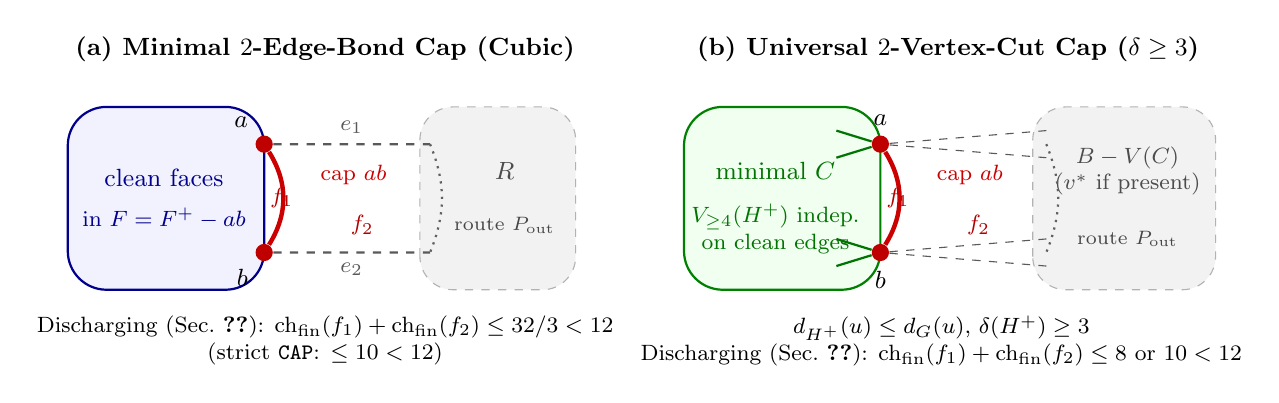
\begin{tikzpicture}[scale=0.86, every node/.style={font=\small}]
  % Left panel: Minimal 2-Edge-Bond Cap (Cubic Planar)
  \begin{scope}[shift={(0,0)}]
    \node[font=\bfseries\small] at (3.8, 3.85) {(a) Minimal $2$-Edge-Bond Cap (Cubic)};
    % Outer shore R (dashed)
    \draw[rounded corners=12pt, dashed, fill=gray!10, draw=gray!60] (5.2,0.3) rectangle (7.5,3.0);
    \node[gray!60!black] at (6.45,2.05) {$R$};
    \node[gray!55!black, font=\scriptsize] at (6.45,1.25) {route $P_{\mathrm{out}}$};
    % Inner shore F
    \draw[rounded corners=14pt, fill=blue!5, draw=blue!55!black, thick] (0.0,0.3) rectangle (2.9,3.0);
    \node[blue!55!black] at (1.42,1.95) {clean faces};
    \node[blue!55!black, font=\footnotesize] at (1.42,1.35) {in $F = F^+ - ab$};
    % Terminals a, b
    \node[circle, fill=red!75!black, inner sep=2.2pt, label=above left:{$a$}] (a) at (2.9,2.45) {};
    \node[circle, fill=red!75!black, inner sep=2.2pt, label=below left:{$b$}] (b) at (2.9,0.85) {};
    % Cut edges e1, e2 and external path P_out
    \draw[dashed, thick, gray!70!black] (a) -- node[above, font=\footnotesize]{$e_1$} (5.35,2.45);
    \draw[dashed, thick, gray!70!black] (b) -- node[below, font=\footnotesize]{$e_2$} (5.35,0.85);
    \draw[dotted, thick, gray!75!black] (5.35,2.45) to[bend left=22] (5.35,0.85);
    % Artificial cap edge ab
    \draw[red!80!black, ultra thick] (a) to[bend left=32] (b);
    % Frozen faces f1, f2 & cap label
    \node[red!70!black, font=\footnotesize] at (3.16,1.65) {$f_1$};
    \node[red!80!black, font=\footnotesize] at (4.22,2.0) {cap $ab$};
    \node[red!70!black, font=\footnotesize] at (4.35,1.25) {$f_2$};
    % Caption strip
    \node[font=\footnotesize, align=center] at (3.8,-0.45) {Discharging (Sec.~\ref{sec:cubic}): $\chf(f_1)+\chf(f_2) \le 32/3 < 12$\\(strict $\texttt{CAP}$: $\le 10 < 12$)};
  \end{scope}

  % Right panel: Universal 2-Vertex-Cut Cap (General Planar delta >= 3)
  \begin{scope}[shift={(9.1,0)}]
    \node[font=\bfseries\small] at (3.9, 3.85) {(b) Universal $2$-Vertex-Cut Cap ($\delta \ge 3$)};
    % Outer part B - V(C)
    \draw[rounded corners=12pt, dashed, fill=gray!10, draw=gray!60] (5.15,0.3) rectangle (7.85,3.0);
    \node[gray!60!black, align=center, font=\footnotesize] at (6.55,2.05) {$B - V(C)$\\($v^*$ if present)};
    \node[gray!55!black, font=\scriptsize] at (6.55,1.05) {route $P_{\mathrm{out}}$};
    % Inner component C
    \draw[rounded corners=14pt, fill=green!6, draw=green!50!black, thick] (0.0,0.3) rectangle (2.9,3.0);
    \node[green!45!black] at (1.35,2.05) {minimal $C$};
    \node[green!45!black, font=\footnotesize, align=center] at (1.35,1.2) {$\Vge(H^+)$ indep.\\on clean edges};
    % Cut vertices a, b
    \node[circle, fill=red!75!black, inner sep=2.2pt, label=above:{$a$}] (a2) at (2.9,2.45) {};
    \node[circle, fill=red!75!black, inner sep=2.2pt, label=below:{$b$}] (b2) at (2.9,0.85) {};
    % Edges into C and outside
    \draw[green!45!black, thick] (a2) -- (2.25,2.65) (a2) -- (2.25,2.25);
    \draw[green!45!black, thick] (b2) -- (2.25,1.05) (b2) -- (2.25,0.65);
    \draw[dashed, gray!70!black] (a2) -- (5.35,2.65) (a2) -- (5.35,2.25);
    \draw[dashed, gray!70!black] (b2) -- (5.35,1.05) (b2) -- (5.35,0.65);
    \draw[dotted, thick, gray!75!black] (5.35,2.45) to[bend left=22] (5.35,0.85);
    % Cap edge ab
    \draw[red!80!black, ultra thick] (a2) to[bend left=32] (b2);
    \node[red!70!black, font=\footnotesize] at (3.16,1.65) {$f_1$};
    \node[red!80!black, font=\footnotesize] at (4.22,2.0) {cap $ab$};
    \node[red!70!black, font=\footnotesize] at (4.35,1.25) {$f_2$};
    \node[font=\footnotesize, align=center] at (3.8,-0.45) {$d_{H^+}(u)\le d_G(u)$, $\delta(H^+)\ge 3$\\Discharging (Sec.~\ref{sec:trilogy}): $\chf(f_1)+\chf(f_2) \le 8$ or $10 < 12$};
  \end{scope}
\end{tikzpicture}
\caption{Connectivity-cap reductions: (a)~Minimal $2$-Edge-Bond Cap (Lemma~\ref{lem:cubic-cap}) for cubic planar graphs, and (b)~Universal $2$-Vertex-Cut Cap (Lemma~\ref{lem:general-cap}) for general planar graphs with $\delta \ge 3$ (where $v^*$ exists only if the leaf block $B$ has a cut-vertex of $G_0$). The terminals $a, b$ are joined by the artificial cap edge $ab$ routed along the external path $P_{\mathrm{out}}$. Cycles using $ab$ are \emph{not} excluded; only the two incident faces $f_1, f_2$ are frozen while every clean face avoids $ab$. The displayed frozen-charge bounds are proved in Sections~\ref{sec:cubic} and~\ref{sec:trilogy}.}\label{fig:caps}
\end{figure}

%% =============================================================================
\section{Main Theorem 1: All Cubic Planar Graphs Contain \texorpdfstring{$C_4, C_8, C_{16},$ or $C_{32}$}{C4, C8, C16, or C32}}\label{sec:cubic}
%% =============================================================================

Suppose for contradiction that $G$ is a finite nonempty simple cubic planar graph containing no simple cycle in $\{C_4, C_8, C_{16}, C_{32}\}$. Apply Lemma~\ref{lem:cubic-cap} to obtain a $3$-connected cubic plane graph $F^+$ with at most two frozen faces $\Ffrz(F^+) \subseteq \{f_1, f_2\}$ sharing the cap edge $ab$, such that every cycle avoiding $ab$ avoids $\{C_4, C_8, C_{16}, C_{32}\}$. By Lemma~\ref{lem:plane-basics}(iii), any two distinct faces of $F^+$ share at most one edge. Assign every face $f$ initial Euler charge
\[
  \chz(f) := 6 - d(f), \qquad \text{so that } \sum_{f} \chz(f) = 12 \quad \text{by~\eqref{eq:euler-cubic}.}
\]
Clean faces have degrees in $\{3, 5, 6, 7, 9, 10, 11, 12, 13, 14, 15, 17, \dots, 31, 33, \dots\}$ (no clean $4$-, $8$-, $16$-, or $32$-faces). Only clean $3$-faces ($+3$) and clean $5$-faces ($+1$) carry positive initial charge.

\subsection{Boundary-Weld Quotient Soundness}\label{subsec:weld-soundness}

To certify local structural exclusions on clean patches inside $F^+$ without risking hidden vertex or edge coincidences, we enumerate planar boundary-weld quotients via \texttt{enum\_planar\_welds} in \texttt{cert/verify\_planar\_eg.py}. For any oriented face-list $\mathcal{P} = (F_1, \dots, F_m)$ (where every face is a simple cycle of length $\ge 3$, every shared undirected edge appears with opposite dart orientations in its two incident faces, and every vertex $v$ has corner multiplicity $c(v) \in \{1, 2, 3\}$), let $p(v)$ be the number of internal edges (used by two faces of $\mathcal{P}$) incident to $v$, and let $e(v)$ be the number of exposed boundary edges (used by one face of $\mathcal{P}$) incident to $v$. Because each facial corner at $v$ contributes two incident darts,
\begin{equation}\label{eq:dart-parity}
  2 p(v) + e(v) \;=\; 2 c(v), \qquad\text{hence } e(v) \;=\; 2\bigl(c(v) - p(v)\bigr) \;\in\; 2\mathbb{Z}_{\ge 0}.
\end{equation}
Call $\mathcal{P}$ \emph{boundary-regular} if (a)~its face-edge contact graph is connected, and (b)~every vertex $v$ satisfies $c(v) - p(v) \in \{0, 1\}$ (equivalently $e(v) \in \{0, 2\}$) and the one-way implication $e(v) = 0 \implies c(v) = 3$. (Note that an intermediate state may have $c(v) = 3$ with $e(v) = 2$ prior to boundary zipping; the stronger biconditional $e(v) = 0 \iff c(v) = 3$ holds for every fully realized quotient $\Phi(\mathcal{P}_0)$ in cubic $F^+$.) Direct instrumentation in \texttt{cert/verify\_parity\_and\_dp.py} verifies that all $844/844$ production seeds passed to \texttt{enum\_planar\_welds} in \texttt{cert/verify\_planar\_eg.py} satisfy boundary-regularity ($722/844$ also satisfy the stronger biconditional).

\begin{lemma}[Soundness and Completeness of Planar Boundary-Weld Enumeration]\label{lem:weld-sound}
Let $\mathcal{P}_0 = (F_1, \dots, F_m)$ be a boundary-regular oriented face-list representing a candidate local configuration of $m$ distinct clean faces of $F^+$ glued along prescribed shared edges, and let $\Phi : V(\mathcal{P}_0) \to V(F^+)$ be the map induced by an actual embedding of those $m$ faces in $3$-connected cubic $F^+$. Then:
\begin{enumerate}[label=(\roman*),leftmargin=2.2em]
  \item Every vertex identification $\Phi(u) = \Phi(v)$ ($u \neq v$) forces the identification of two oppositely oriented exposed boundary darts at that vertex. Moreover, every partial boundary-weld quotient $\mathcal{Q}$ subordinate to $\Phi$ (obtained from $\mathcal{P}_0$ by welding a subset of boundary-edge pairs identified under $\Phi$) preserves boundary-regularity through every merge wave of \texttt{weld\_boundary}: specifically, every vertex satisfies $e(v) \in \{0, 2\}$ and $e(v) = 0 \implies c(v) = 3$, and whenever $c(v) = 3$ with $e(v) = 2$, cubicity uniquely forces the two exposed boundary darts at $v$ to be opposite sides of the same edge of $F^+$.
  \item The realized image $\Phi(\mathcal{P}_0)$ is connected, satisfies $e(v) = 0 \iff c(v) = 3$ at every vertex, and its exposed boundary edges form a vertex-disjoint union of $h \ge 0$ simple boundary circles bounding $h$ open disks in $S^2 \setminus \Phi(\mathcal{P}_0)$, whence $\Phi(\mathcal{P}_0)$ satisfies the spherical Euler equation $V - E + F = 2 - h$ as well as $|F_i \cap F_j| \in \{0, 2\}$ matching a unique shared edge (Lemma~\ref{lem:plane-basics}(iii)).
  \item Separating \emph{hereditary pruning} (invalid \texttt{patch\_data}: non-simple face, corner multiplicity $> 3$, repeated face-pair contact, non-opposite dart orientation, or \texttt{weld\_boundary} failure) from \emph{emit-only validity filters} (the Euler test $V - E + F = 2 - h$ and exact face-intersection check) guarantees that $\Phi(\mathcal{P}_0)$ is isomorphic to one of the quotients emitted by \texttt{enum\_planar\_welds}$(\mathcal{P}_0)$.
  \item Conversely, if every emitted quotient $W$ satisfies strict face-schema validity (\texttt{WeldSchemaValid}: dense labels $0,\dots,n_W-1$, all faces simple of length $\ge 3$) and contains a simple cycle $C$ of length $L \in \{4, 8, 16, 32\}$ in the edge union of its face boundaries, then the image of $C$ in $F^+$ is a genuine simple cycle of length $L$ avoiding $ab$ in the edge union of the $m$ clean facial boundaries in $F^+ - ab \subseteq G$.
\end{enumerate}
\end{lemma}

\begin{proof}
(i) Because $F^+$ is $3$-connected and cubic, Lemma~\ref{lem:plane-basics}(iii) implies that two distinct faces of $F^+$ share a vertex $z$ if and only if they share an edge incident to $z$. Hence if $\Phi$ identifies two distinct vertices of a quotient $\mathcal{Q}$, their incident faces share an edge in $F^+$ that is not yet welded in $\mathcal{Q}$, so two oppositely oriented exposed boundary edges of $\mathcal{Q}$ map to the same edge of $F^+$.

We prove by induction on iterations of \texttt{weld\_boundary} that for any boundary-regular quotient $\mathcal{Q}$ subordinate to $\Phi$ and any pair of exposed boundary darts $(i, u, v)$ and $(j, w, x)$ mapping to opposite darts of the same edge of $F^+$, every merge wave preserves $e(z) \in \{0, 2\}$ and $e(z) = 0 \implies c(z) = 3$. In wave~$1$, identifying $(u, v)$ with $(x, w)$ merges $u \sim x$ and $v \sim w$. Because $\Phi(u) = \Phi(x)$ and $\Phi(v) = \Phi(w)$ are the two distinct endpoints of the edge $\Phi(uv) = \Phi(xw)$ in simple $F^+$, the two endpoint merge classes $\{u, x\}$ and $\{v, w\}$ have distinct $\Phi$-images and are disjoint. Since $u, x$ each have an exposed dart before the merge, $c(u) - p(u) = c(x) - p(x) = 1$; after merging, the newly paired edge $(u, v) \sim (x, w)$ increases the internal edge count by at least $1$, so the merged vertex $z = \{u, x\}$ satisfies
\[
  c(z) - p(z) \;\le\; \bigl(c(u) - p(u)\bigr) + \bigl(c(x) - p(x)\bigr) - 1 \;=\; 1 + 1 - 1 \;=\; 1.
\]
By~\eqref{eq:dart-parity}, $e(z) = 2(c(z) - p(z)) \in \{0, 2\}$. Whenever a vertex $z$ has $c(z) = 3$ and $e(z) = 2$, its three facial corners already account for all three faces around $\Phi(z)$ in cubic $F^+$, so its two exposed boundary edges $(z, t_1)$ and $(z, t_2)$ must be the two opposite darts of the third edge of $F^+$ at $\Phi(z)$, forcing $\Phi(t_1) = \Phi(t_2)$ (so the zipping pair $(t_1, t_2)$ in \texttt{pending} is subordinate to $\Phi$). In any subsequent zipping wave, let $K$ be a connected component of vertices merged together by the pairs in \texttt{pending}. Every vertex $y \in K$ is a tip of an exposed dart, so $c(y) - p(y) = 1$, and no $c = 3$ vertex $z$ can belong to $K$ (merging it with another vertex would give $c \ge 4$, impossible under $\Phi$). A spanning tree of $K$ has $|K| - 1$ edges, each emitted by a distinct $c = 3$ vertex $z_r \notin K$ (since each $c = 3$ vertex emits at most one pair $(t_1, t_2)$), yielding $|K| - 1$ distinct newly paired internal edges $(z_r, K)$ incident to the merged vertex $K$. Hence
\[
  c(K) - p(K) \;\le\; \sum_{y \in K} \bigl(c(y) - p(y)\bigr) - (|K| - 1) \;=\; |K| - (|K| - 1) \;=\; 1,
\]
so $e(K) = 2(c(K) - p(K)) \in \{0, 2\}$. Finally, if $e(K) = 0$ then $c(K) = p(K)$, meaning the $c(K)$ facial corners at $K$ form a closed cyclic fan of distinct simple faces around $\Phi(K)$ in cubic $F^+$; in a simple cubic plane graph, every vertex has degree $3$ and lies in exactly $3$ faces, forcing $c(K) = 3$. Thus \texttt{weld\_boundary} never rejects a partial quotient subordinate to $\Phi$.

(ii) Because $\mathcal{P}_0$ is face-edge-connected, the union $U := \bigcup_{i=1}^m \overline{\Phi(F_i)} \subset S^2$ is connected. In the fully realized quotient $\Phi(\mathcal{P}_0)$, all three incident edges at any $c(v) = 3$ vertex are already identified under $\Phi$, so $c(v) = 3 \implies e(v) = 0$ as well, giving $e(v) = 0 \iff c(v) = 3$. At every vertex $z$ of $\Phi(\mathcal{P}_0)$, the $c(z) \in \{1, 2, 3\}$ incident facial wedges of $U$ form a contiguous subset in the cyclic rotation $\sigma_z$ around the cubic vertex $z$ (every nonempty subset of a $3$-element cycle is contiguous); hence $U$ is locally a topological $2$-manifold with boundary, and its exposed boundary edges ($e(v) = 2$) form a vertex-disjoint union of $h \ge 0$ simple closed boundary circles, each separating an empty region of $S^2 \setminus U$ from the connected face union $U$. Because $U$ is connected on $S^2$, every connected component of $S^2 \setminus U$ is simply connected (an open topological disk) bounded by one of these $h$ simple boundary circles. Capping each of the $h$ boundary circles with a disk face yields a cellular decomposition of $S^2$ with $V$ vertices, $E$ edges, and $F + h$ faces, so Euler's formula~\eqref{eq:euler-general} gives $V - E + (F + h) = 2$, i.e., $V - E + F = 2 - h$. Exact face intersection $|F_i \cap F_j| \in \{0, 2\}$ holds by Lemma~\ref{lem:plane-basics}(iii).

(iii) Every hereditary pruning condition is preserved under subordination to $\Phi$: any partial quotient subordinate to $\Phi$ inherits face simplicity, corner multiplicity $\le 3$, at most one shared edge per face pair, opposite dart orientations, and (by~(i)) \texttt{weld\_boundary} closure. Starting from $\mathcal{P}_0$ and repeatedly picking any pair of distinct exposed boundary edges identified under $\Phi$ yields a finite chain of valid \texttt{weld\_boundary} transitions terminating at $\Phi(\mathcal{P}_0)$ (since when no two exposed boundary edges map to the same edge, Lemma~\ref{lem:plane-basics}(iii) implies $\Phi$ is injective on vertices). Applying the non-hereditary Euler and exact-contact filters strictly at emission time guarantees that $\Phi(\mathcal{P}_0)$ is reached and emitted.

(iv) By~(iii), \texttt{enum\_planar\_welds}$(\mathcal{P}_0)$ emits a representative quotient $W_0$ isomorphic to the realized patch $\Phi(\mathcal{P}_0)$, whose face-boundary edge union is isomorphic to the edge union of the $m$ clean facial boundaries in $F^+ - ab \subseteq G$. Applying the universal hypothesis over all emitted quotients to $W_0$ supplies a strict-schema simple cycle $C$ of length $L \in \{4, 8, 16, 32\}$ in the edge union of the face boundaries of $W_0$, which lifts through the isomorphism $W_0 \cong \Phi(\mathcal{P}_0)$ to a genuine simple cycle of length $L$ in $F^+ - ab \subseteq G$ (additional edges of $F^+$ between vertices of $\Phi(\mathcal{P}_0)$ only add chords and never affect simplicity of $C$).
\end{proof}

\subsection{Clean Clusters, \texorpdfstring{$51$}{51} Mixed Chains, and Complete Charge-Conserving Discharging Rules}\label{subsec:cubic-rules}

In $F^+$, no two clean $3$-faces share an edge ($3+3-2 = 4$), and no two clean $5$-faces share an edge ($5+5-2 = 8$). Moreover, no clean $3$-face $T_2$ can share edges with two distinct clean $5$-faces $P_1, P_2$: those two edges meet at a cubic vertex of $T_2$, so $P_1$ and $P_2$ share that cubic vertex and hence by Lemma~\ref{lem:plane-basics}(iii) share an edge, forming a simple $C_8$ ($5+5-2=8$). Likewise, a clean $5$-face cannot touch three clean $3$-faces (by pigeonhole on $C_5$, two of the $3$-faces would share a vertex and hence an edge, creating $C_4$). Consequently, the maximal edge-connected clusters of clean $\{3,5\}$-faces have size at most $3$, are pairwise vertex-disjoint (by Lemma~\ref{lem:plane-basics}(iii), if two clusters shared a vertex they would share an edge), and fall into five types:
\begin{itemize}[leftmargin=1.8em]
  \item Isolated clean $3$-faces $T$ ($\chz = +3$) and isolated clean $5$-faces $P$ ($\chz = +1$);
  \item Pairs $TP$ ($\chz = +4$): a clean $3$-face $T$ and clean $5$-face $P$ sharing an edge $uv$. Its four outer faces are the two \emph{side faces} $S_1, S_2$ meeting opposite ends $u, v$ of the shared edge $uv$ (each sharing one edge with $T$ and one edge with $P$, and meeting each other along an edge at the third vertex of $T$), and the two \emph{bottom faces} $B_1, B_2$ on the remaining two edges of $P$ (with $B_1$ adjacent to $S_2$ and $B_2$ adjacent to $S_1$, meeting each other at the vertex of $P$ opposite $uv$);
  \item Triples $TPT$ ($\chz = +7$): a clean $5$-face flanked by two non-adjacent clean $3$-faces, with one \emph{apex face} $A$ (width $3$ on $TPT$, sharing an edge with both triangles and the pentagon edge between them) and two \emph{flank faces} $B, C$ (each width $2$ on $TPT$, sharing one edge with a triangle and one with the pentagon, and sharing an edge with each other at the fifth pentagon vertex);
  \item Super-gadgets $S = TPT_1 + F_9 + TPT_2$ ($\chz = 7 + 7 - 3 = +11$): formed whenever a clean $9$-face $F_9$ serves as the $A$-face of two distinct $TPT$ clusters, with three outer $\ge 17$/frozen receiver faces $X$ (width $5$, bridging both $TPT$s across one edge of $F_9$) and $Y, Z$ (each width $3$, meeting the other two free edges of $F_9$ at a single common cubic vertex $w_8$ incident only to $F_9, Y, Z$).
\end{itemize}
Clean $6$-faces carry initial charge $0$ and act as relays. Because adjacent $(3,3)$ ($C_4$), adjacent $(5,5)$ ($C_8$), and clean $6$-faces on either side face $S_1, S_2$ of $TP$ or any of the $7$ boundary edges of $TPT$ ($C_8$) are forbidden, every clean $6$-face $H_6$ touches at most one clean $3$-face ($6 + 2 = 8$) and belongs to at most one positive-cluster charge source: \emph{Corannulene pent-hex} $6_c$ (adjacent to a $(6,6,6,6,6)$ isolated $P$), \emph{tri-hex} ($6_s$ sharing a triangle $T$ directly along a receiver boundary, or $6_o$ transmitting charge from a triangle $T$ across an outer edge of $H_6$), or \emph{$TP$-bottom hex} $TP_6$ (on $B_1 = 6$ of a $TP(S_2=9, B_2=9)$ cluster with $S_1 \ge 33$ or frozen and no triad triangle on $B_1$). In particular, if $H_6$ forms a clean $(3,6,5)$-triad (touching both a clean $3$-face and a clean $5$-face), structural welding shows that the $5$-face ($P$ or $TP$) always sends $0$ charge to $H_6$, so $H_6$ receives charge exclusively from its unique clean $3$-face.

\subsubsection*{Deterministic Charge-Conserving Discharging Rules (Three Stages)}
Fix an arbitrary canonical total ordering $\prec$ on $F(F^+)$ to break ties deterministically. Every rule below applies uniformly whether $0, 1,$ or $2$ frozen faces appear in the cluster neighborhood, and every rule preserves total charge identically.

\medskip
\noindent\textbf{Stage 1A --- Isolated clean $3$-face $T$ ($\chz = +3$, neighbors $X, Y, Z$):}
\begin{enumerate}[label=(T\arabic*),leftmargin=2.8em]
  \item \emph{Two frozen neighbors ($f_1, f_2, Z$; token $T_{\mathrm{frz}}$):} This occurs only when $T$ contains an endpoint $a$ or $b$ of $ab$ (at most two such triangles). Send $3/2$ to $f_1$, $3/2$ to $f_2$, and $0$ to $Z$. (Total $3/2 + 3/2 = 3$.)
  \item \emph{Three clean $6$-faces $(6, 6, 6)$ (Mini-Corannulene):} Send $1$ to each of the three $6$-faces (routed in Stage~3 across its three valleys and flanking opposite faces as below). (Total $1 + 1 + 1 = 3$.)
  \item \emph{Two clean $6$-faces $(6, 6, X)$ (token $T_2$ on $X$):} Clean $X$ has $d(X) \in \{9, 10, 11, 14\} \cup [17, \infty)$ (since $3+6+d-6 \in \{4,8,16\}$ or $6+d-2=16$ forbids $7,12,13,15$), or $X \in \Ffrz$. Send $(1, 1, 1)$ to $(6, 6, X)$ if $X$ is clean $9$; send $(0, 0, 3)$ if $X$ is clean $11$; send $(1/2, 1/2, 2)$ if $X$ is clean $10, 14, \ge 17$ or frozen. (Total $3$.)
  \item \emph{One clean $6$-face $(6, X, Y)$ (token $T_1$ on $X, Y$):} Clean $X, Y$ lie in $\{9, 10, 11, 14\} \cup [17, \infty)$ or $\Ffrz$; neither $(9,9)$ ($C_{16}$) nor $(9,10)$ ($3+9+10-6=16$) occurs. Define $w_1(d) = 3/4$ ($d=9$), $1$ ($d=10$), $3/2$ ($d \in \{11, 14\} \cup [17, \infty)$ or frozen). If at least one of $X, Y$ is clean $11$ (say $X = 11$, choosing the $\prec$-first if both are $11$), send $0$ to $6$, $w_1(Y)$ to $Y$, and $3 - w_1(Y) \in \{9/4, 2, 3/2\} \le 9/4$ to $X$. Otherwise send $w_1(X)$ to $X$, $w_1(Y)$ to $Y$, and $3 - w_1(X) - w_1(Y) \in \{0, 1/2, 3/4, 1\}$ to $6$ (nonnegative since $w_1(X) + w_1(Y) \le 3$, and $\le 1$ since $(9,9)$ and $(9,10)$ are forbidden). (Total $3$.)
  \item \emph{Zero clean $6$-faces $(X, Y, Z)$ (tokens $T, T_{10}, T_{L9}, T_{R9}$):} Each neighbor is frozen or clean in $\{9, 10, 11, 12, 13, 14\} \cup [17, \infty)$ (no $7, 15$). At most one is clean $9$ ($9+9-2=16$), and if one is clean $9$ neither other is clean $10$ ($3+9+10-6=16$). If one neighbor is clean $9$, send $3/4$ to it and $9/8$ to each of the other two ($3/4 + 9/8 + 9/8 = 3$); otherwise send $1$ to each of $X, Y, Z$ ($1 + 1 + 1 = 3$; note $1 \le 9/8$, and when adjacent to a $5$-triangle clean $10$-face $R_{10}$ the other two neighbors record $T_{10}$ of weight $1$).
\end{enumerate}

\noindent\textbf{Stage 1B --- Isolated clean $5$-face $P$ ($\chz = +1$):}
\begin{enumerate}[label=(P\arabic*),leftmargin=2.8em]
  \item \emph{Corannulene $(6, 6, 6, 6, 6)$:} Send $1/5$ to each of its $5$ adjacent clean $6$-faces ($6_c$). (Total $5 \cdot 1/5 = 1$.)
  \item \emph{Non-Corannulene $P$:} If $P$ touches at least one frozen face or clean face $X$ with $d(X) \in \{10\} \cup [12, \infty)$, send $+1$ to the $\prec$-first such face $X$ and $0$ to all other neighbors. Otherwise all $5$ neighbors of $P$ are clean in $\{6, 7, 9, 11\}$: because $(6,6,6,6,7)$ ($0/9$ welds), $(6,6,6,6,9)$ ($0/18$ welds), $(6,6,6,6,11)$ ($0/31$ welds), and every clean $\{6, 7, 9, 11\}$-ring containing $\le 1$ neighbor in $\{9, 11\}$ (with a $7$-face or triad $6$-face) die at $\{C_4, C_8, C_{16}, C_{32}\}$ (by cubic boundary welding, Lemma~\ref{lem:weld-sound}), $P$ must touch at least two clean $\{9, 11\}$-faces; send $1/2$ to each of the $\prec$-first two clean $\{9, 11\}$-neighbors and $0$ to all others. (Total $1$; every clean $6$-face and clean $7$-face receives $0$, and frozen neighbors always take the first branch directly without invoking clean cycle exclusions.)
\end{enumerate}

\noindent\textbf{Stage 1C --- Cluster $TP$ ($\chz = +4$, side faces $S_1, S_2$, bottom faces $B_1, B_2$):}
Each side face $S_i$ shares an edge with $T$ and an edge with $P$, so $S_i$ is frozen or clean $\ge 9$ ($3, 4, 5, 6, 7, 8$ are excluded by maximality, $C_4$, and $C_8$ since $3+6-2=7$ and $3+5+6-6=8$ forbid $S_i=6$, and $3+7-2=8$ forbids $S_i=7$), and at most one of $S_1, S_2$ is clean $9$ ($9+9-2=16$). Similarly, at most one of $B_1, B_2$ is clean $9$.
\begin{enumerate}[label=(TP\arabic*),leftmargin=3.2em]
  \item \emph{Neither $S_1$ nor $S_2$ is clean $9$:} Send $(2, 2, 0, 0)$ to $(S_1, S_2, B_1, B_2)$ (regardless of $B_1, B_2$, including when either is $6, 7,$ or frozen). (Total $2 + 2 = 4$.)
  \item \emph{One side face is clean $9$ (say $S_2 = 9$, so $S_1$ is frozen or clean $\ge 11$ by $3+9+10-6=16$):} Send $3/4$ to $S_2 = 9$ and distribute the remaining $13/4$ as follows:
  \begin{itemize}[leftmargin=1.5em]
    \item If neither $B_1$ nor $B_2$ is clean $6$ or $7$: send $2$ to $S_1$; if one bottom is clean $9$ and the other is $\ge 10$/frozen, send $(1/4, 1)$ to them; if both bottoms are $\ge 10$/frozen, send $1$ to the $\prec$-first and $1/4$ to the other. (Total $3/4 + 2 + 1 + 1/4 = 4$.)
    \item If one bottom is clean $7$: the other bottom $B'$ is frozen or clean $\ge 14$ (since $B'$ shares a vertex with $B=7$ and $P=5$, clean $6, 7, 9, 10, 11, 12, 13$ yield $5+7+d-6 \in \{16\}$ or $C_4/C_8/C_{16}/C_{32}$ welds, while a frozen $B'$ satisfies this branch directly); send $2$ to $S_1$, $0$ to the $7$-face, and $5/4$ to $B'$ (token $TP_{b54}$, or fused length-$3$ token $HH$ of weight $5/2$ when two $TP_{b54}$ clusters share the same separating $7$-face edge along $B'$). (Total $3/4 + 2 + 5/4 = 4$.)
    \item If one bottom is clean $6$: by the $16$ $S_2=9, B_2=6$ seal welds (Proposition~\ref{prop:51chains}(iii)), only $B_1$ (adjacent to $S_2=9$) can be clean $6$, and $B_2$ is either clean $9$ or frozen/clean $\ge 14$ (clean $6, 7, 10, 11, 12, 13$ yield $C_{16}/C_{32}$ perimeters with $B_1=6, P=5, S_2=9$, while frozen $B_2$ takes the first subbranch directly). If $B_2$ is frozen or clean $\ge 14$, send $2$ to $S_1$, $0$ to $B_1 = 6$, and $5/4$ to $B_2$ ($TP_{b54}$; total $4$). If $B_2 = 9$, then $TP(B_1=6, S_2=9, B_2=9)$ has unique surviving weld shift spectrum $\texttt{sh\_TP699} = (0..3, 5..14)$ on $S_1$ (out of $21$ welds), eliminating clean $S_1 \in \{18..20, 22, 24..27, 29..31\}$ (and $11, 13, 14, 15$ by $C_{16}$), leaving $S_1 \in \{12, 17, 21, 23, 28\} \cup [33, \infty) \cup \Ffrz$: if $S_1 \in \{12, 17, 21, 23, 28\}$, send $3$ to $S_1$ ($TP_s=3$ at $d=12$; width-$4$ $TP_{s3}=3$ at $d \in \{17,21,23,28\}$) and $0$ to $B_1$; if $S_1 \ge 33$ or frozen and $B_1=6$ touches a triad triangle on its $(8,9)$ edge, send $3$ to $S_1$ (width-$4$ $TP_{s3,t89}$) and $0$ to $B_1$; otherwise send $7/3$ to $S_1$ (width-$2$ $TP_{s73}$) and $2/3$ to $B_1=6$ (relayed via $TP_6$ in Stage~3). (Total $3/4 + 1/4 + 7/3 + 2/3 = 4$.)
  \end{itemize}
\end{enumerate}

\noindent\textbf{Stage 1D --- Cluster $TPT$ ($\chz = +7$) and Super-Gadget $S$ ($\chz = +11$):}
Every outer face $A, B, C$ of $TPT$ shares edges with a clean triangle and clean pentagon, so each is frozen or clean $\ge 9$ ($3, 4, 5, 6, 7, 8$ excluded by maximality, $C_4$, $C_8$), and at most one is clean $9$ ($9+9-2=16$). Whenever a flank or apex face is frozen, it automatically satisfies every $\ge 10/\Ffrz$, $\ge 11/\Ffrz$, or $\ge 17/\Ffrz$ condition below without requiring any clean cycle witness on that face:
\begin{enumerate}[label=(TPT\arabic*),leftmargin=3.6em]
  \item \emph{Super-gadget $S = TPT_1 + F_9 + TPT_2$ ($+11$):} Its three outer faces $X, Y, Z$ are clean $\ge 17$ or frozen (clean $9..15$ on $X, Y, Z$ produce $C_{16}$ or $C_{32}$ with the $7$-face cluster $S$ whose shift spectra are $\texttt{sh\_X}, \texttt{sh\_Y}$). Send $9/2$ to $X$ ($S_X$, width $5$) and $13/4$ to each of $Y, Z$ ($S_{YZ}$, width $3$). (Total $9/2 + 13/4 + 13/4 = 11$.)
  \item \emph{Standard $TPT$ ($+7$, not in $S$):}
  \begin{itemize}[leftmargin=1.5em]
    \item $A = 9$ ($B, C \ge 17$ or frozen, since $TPT + F_9$ has shift spectrum $\texttt{sh\_A9}$ killing clean $10..15$): send $3/2$ to $A$ and $11/4$ each to $B, C$ ($TPT_{A9}$, width $3$). (Total $7$.)
    \item $A = 10$ ($B, C \ge 17$ or frozen, since $TPT + F_{10}$ has shift spectrum $\texttt{sh\_A10} = (0..9)$ killing clean $9..15$): send $2$ to $A$ and $5/2$ each to $B, C$ ($TPT_{A10}$, width $3$). (Total $7$.)
    \item $B = 9$ w.l.o.g.\ ($A \ge 17$/frozen and $C \in \{11\} \cup [17,\infty) \cup \Ffrz$, since $TPT + F_{B9}$ has shift spectra $\texttt{sh\_B9\_A}, \texttt{sh\_B9\_C}$ killing all other clean degrees $\le 15$): send $3/2$ to $B$, $23/8$ to $A$ ($TPT_{B9A}$, width $4$), and $21/8$ to $C$ ($TPT_{B9C}$, width $3$; or $TPT_{BC}(11)=21/8$ at $d=11$). (Total $3/2 + 23/8 + 21/8 = 7$.)
    \item $B = 10$ w.l.o.g.\ ($A \in \{12\} \cup [17,\infty) \cup \Ffrz$ by $TPT$ shift $(0..3)$ plus $B=10$ detours, $C \ge 10$/frozen): send $12/5$ to $A$, $23/10$ to $B$, and $23/10$ to $C$ (note $23/10 \le w(TPT_{BC})$ for all $d \ge 10$ and frozen). (Total $12/5 + 23/10 + 23/10 = 7$.)
    \item All of $A, B, C$ clean $\ge 11$ or frozen: send $7/3$ to each of $A, B, C$ (note $7/3 \le w(TPT_A), w(TPT_{BC})$ for all $d \ge 11$ and frozen). (Total $7$.)
  \end{itemize}
\end{enumerate}

\noindent\textbf{Stage 2 --- Clean $10$-Face $5$-Triangle Relay $R_{10}$:}
If a clean $10$-face $F_{10}$ ($\chz = -4$) is adjacent to $5$ clean $3$-faces, those $5$ triangles are non-adjacent ($C_4$) and therefore alternate around $\partial F_{10}$. For each of the $5$ non-triangle gap neighbors $Q$ of $F_{10}$: clean $d(Q) \in \{3, 4, 8, 16, 32\}$ are excluded by $C_4$ and forbidden lengths; clean $d(Q) \in \{5, 6, 7, 9, 10\}$ are eliminated by the $5$ exact $R_{10}$ seal welds (Proposition~\ref{prop:51chains}(iii), matching the $10$-face plus $5$ triangles plus $Q$ sharing its $3$-edge rim with $F_{10}$ and its two flanking triangles); and clean $d(Q) = 15$ is excluded because $Q$ shares an edge with both flanking triangles ($3+15-2=16$). Hence all $5$ gap neighbors $Q$ are frozen or clean with $d(Q) \ge 11$ ($d \neq 15$). Because every vertex of $F_{10}$ is cubic, each gap neighbor $Q$ is simultaneously a neighbor of both flanking triangles, so the no-$6$/no-$9$ exclusion on the five gap neighbors directly establishes that none of the $5$ triangles touches a clean $6$-face or clean $9$-face; hence each triangle lies in Stage~1A(T5) and sends $+1$ to $F_{10}$. This fills $F_{10}$'s initial deficit $-4$ to a net relay surplus of $-4 + 5 = +1$. In Stage~2, $F_{10}$ relays this $+1$ by sending $1/5$ across each of its $5$ non-triangle edges (token $R_{10}$ on each neighbor), leaving $\chf(F_{10}) = -4 + 5 - 1 = 0$. (In the clean $d=10$ cyclic DP at \texttt{verify\_planar\_eg.py:1373}, this exact $-1$ out-transfer is the subtraction \texttt{- W\_LCM} when \texttt{d == 10 and cnt == 5}.)

\noindent\textbf{Stage 3 --- Charged Clean $6$-Faces ($H_6$, $\chz = 0$):}
Every clean $6$-face $H_6$ receives charge from at most one Stage-1 source:
\begin{enumerate}[label=(H\arabic*),leftmargin=2.8em]
  \item \emph{Corannulene $6_c$ ($+1/5$):} Sends $1/10$ across each of its two valley edges, so each valley face ($d \in \{11\} \cup [13, \infty)$ or frozen) receives $1/10 + 1/10 = 1/5$ across its consecutive $6_c\,6_c$ pair. ($\chf(H_6) = 0$.)
  \item \emph{Charged $TP$-bottom hex $TP_6$ ($+2/3$):} Its two outer faces $F_{67}, F_{89}$ lie in $\{10, 11, 13, 14\} \cup [17, \infty) \cup \Ffrz$ with $(F_{67}, F_{89}) \notin \{(10,10), (10,11), (11,10)\}$ (and $F_{78} \notin \{5, 9\}$). If one of $F_{67}, F_{89}$ is clean $10$, send $0$ to it and $2/3$ to the other ($\ge 13$ or frozen); otherwise send $1/3$ to each (bounded by $TP_6$ weight $1/3$ at $d=11$ and $2/3$ at $d \in \{13, 14\} \cup [17, \infty) \cup \Ffrz$). ($\chf(H_6) = 0$.)
  \item \emph{Charged tri-hex $H_6$ ($c(H_6) \in \{3/8, 1/2, 3/4, 1\}$):} For Mini-Corannulene $(6,6,6)$, at least two valleys are clean $\ge 13$ or frozen (each taking $1/2 + 1/2 = 1$ from its two flanking $6$-faces); if the third valley is $\ge 13$/frozen it takes $1/2 + 1/2$, else it is $6$ or $7$ and both flanking opposite faces are $\ge 10$/frozen, each taking $1/2$ from its incident $6$-face (total $3$, every outer edge $\le 1/2$). For every other charged tri-hex $H_6$ ($c(H_6) \le 1$) with outer neighbors $(V_0, O, V_1)$, assign outer-edge receiver capacities $\capf(\Ffrz) = 1$, $\capf(6) = 0$, $\capf(7) = 1/4$ (or $1/2$ in the isolated \texttt{Triad-D1}$(X=10, Z_1=7, Z_2=6)$ patch with base faces $T=(0,1,2)$, $H_6=(2,1,3,4,5,6)$, $P=(4,3,10,11,12)$, $X_{10}=(10,3,1,0,20..25)$, $Z_1=(5,4,12,30,31,32,33)$, $Z_2=(6,5,33,40,41,42)$ [$1/50$ surviving base weld], where attaching a clean $6$-face on each of the $4$ remaining free edges $(12,30)$ [sharing $(11,12)$ with $P$], $(30,31)$, $(31,32)$, and $(32,33)$ [sharing $(33,40)$ with $Z_2$] of $Z_1 = 7$ is eliminated across $106 + 142 + 140 + 73 = 461$ boundary welds with $0$ survivors [verified in \texttt{cert/verify\_parity\_and\_dp.py}], so $Z_1 = 7$ receives only that single $1/2$ and ends with $\chf(Z_1) = -1/2 < 0$), $\capf(9) = 3/4$ (except $0$ if $V_{6,6}$ valley of $(3; 6, 6, X)$), $\capf(10) = 2/3$, $\capf(11) = \capf(12) = 0$, and $\capf(\ge 13) = 1/2$. Notice that any frozen outer neighbor alone has $\capf(\Ffrz) = 1 \ge c(H_6)$; in all-clean neighborhoods (including $(3,6,5)$-triads \texttt{Triad-D1}, \texttt{Triad-Opp}, \texttt{Triad-TPP}), clean boundary-weld exclusions eliminate every low-capacity triple $(V_0, O, V_1)$ with $\capf(V_0) + \capf(O) + \capf(V_1) < c(H_6)$ (in particular, when $c(H_6) = 1$, at least two outer faces have capacity $\ge 1/2$, or one has $3/4$ and another $\ge 1/4$, or $Z_1 = 7$ takes $1/2$ alongside $O = 10$ or $\ge 13$). Allocate $c(H_6)$ greedily across $(V_0, O, V_1)$ in $\prec$-order up to their capacities ($\chf(H_6) = 0$). Finally, for clean $d = 7$: every non-triad-D1 clean $7$-face receives $0$ from all $\{3, 5\}$-clusters and at most $1/4$ per adjacent charged $6$-face ($6_o$); because $3$ consecutive clean $6$-faces on a clean $7$-face with any charging triangle placement die across all $7$ cubic boundary-weld seeds ($0/2..0/5$ survivors), at most $4$ edges of $F_7$ carry a charged $6$-face (by pigeonhole on $C_7$, any $5$ of $7$ edges contain $3$ consecutive edges), giving $\chf(F_7) \le -1 + 4 \cdot \frac{1}{4} = 0$ directly (while the $d=7$ DP also checks all mixed chains containing $6_o$).
\end{enumerate}

By inspection of (T1)--(T5), (P1)--(P2), (TP1)--(TP2), (TPT1)--(TPT2), Stage~2, and (H1)--(H3), every sender's net outgoing charge equals its Stage-1/2/3 balance (yielding $\chf(f) = 0$ for all clean $3$-, $5$-, $6$-faces, and $R_{10}$ relays), and every receiving clean or frozen face records at most the exact rational token weights summarized in Table~\ref{tab:cubic-weights}.

\begin{table}[t]
\centering
\caption{Exact cubic discharging token weights (in exact rationals) received by a clean $d$-face or frozen face ($d \ge 3$), matching \texttt{verify\_planar\_eg.py:942--1029, 1403--1430, 1494--1535}. A dash (\,---) indicates the token is absent at that degree; $0$ indicates a present zero-weight token.}\label{tab:cubic-weights}
\scriptsize
\setlength{\tabcolsep}{3pt}
\resizebox{\textwidth}{!}{%
\begin{tabular}{@{}lcccccccccc@{}}
\toprule
Token & Width & $d=7$ & $d=9$ & $d=10$ & $d=11$ & $d=12$ & $d=13$ & $d=14$ & Clean $d\ge 17$ & Frozen \\
\midrule
$T$ & $1$ & $0$ & $3/4$ & $1$ & $9/8$ & $9/8$ & $9/8$ & $9/8$ & $9/8$ & $9/8$ \\
$T_{10}$ & $1$ & --- & --- & --- & $1$ & $1$ & $1$ & $1$ & $1$ & $1$ \\
$P$ & $1$ & $0$ & $1/2$ & $1$ & $1/2$ & $1$ & $1$ & $1$ & $1$ & $1$ \\
$TP_b$ & $1$ & $0$ & $1/4$ & $1$ & $1$ & $1$ & $1$ & $1$ & $1$ & $1$ \\
$TP_s$ (std.) & $2$ & $0$ & $3/4$ & $2$ & $2$ & $3$ & $2$ & $2$ & $2$ & $2$ \\
$TP_{b54}$ / $HH$ & $2 / 3$ & --- & --- & --- & --- & --- & --- & $5/4,\ 5/2$ & $5/4,\ 5/2$ & $5/4,\ 5/2$ \\
$TPT_A$ / $TPT_{BC}$ (std.) & $3 / 2$ & $0,\ 0$ & $3/2,\ 3/2$ & $2,\ 23/10$ & $7/3,\ 21/8$ & $12/5,\ 7/3$ & $12/5,\ 7/3$ & $12/5,\ 7/3$ & $12/5,\ 7/3$ & $12/5,\ 7/3$ \\
$T_1$ / $T_2$ & $2 / 3$ & --- & $3/4,\ 1$ & $1,\ 2$ & $9/4,\ 3$ & --- & --- & $3/2,\ 2$ & $3/2,\ 2$ & $3/2,\ 2$ \\
$6_o$ & $1$ & $1/4$ ($\le 4$; sole $1/2$) & $3/4$ & $2/3$ & --- & --- & $1/2$ & $1/2$ & $1/2$ & $1$ \\
$TP_{6,L/R}$ / $TP_{6,2}$ & $2 / 3$ & --- & --- & --- & $1/3,\ 2/3$ & --- & $2/3,\ 4/3$ & $2/3,\ 4/3$ & $2/3,\ 4/3$ & $2/3,\ 4/3$ \\
$R_{10}$ & $1$ & --- & --- & --- & $1/5$ & $1/5$ & $1/5$ & $1/5$ & $1/5$ & $1/5$ \\
$6_c$ ($+1/5$ on $6_c6_c$) & $1$ & --- & --- & --- & $0$ & --- & $0$ & $0$ & $0$ & $0$ \\
$T_{\mathrm{frz},L/R}$ / $\texttt{CAP}$ & $1 / 0$ & --- & --- & --- & --- & --- & --- & --- & --- & $3/2,\ 0$ \\
\bottomrule
\end{tabular}}
\smallskip

\raggedright\footnotesize
\emph{Notes:} (1)~At clean $d = 15$, $T, T_{10}, R_{10}, T_1, T_2, TP_6$ are absent ($3+15-2=16$, $6+15-2+3$-detours); $P, TP_b, TP_s, TP_{b54}, HH, TPT_A, TPT_{BC}$ retain their $d=14$ weights, $6_o$ has weight $1/2$, and $6_c$ ($+1/5$ pair bonus) is present. (2)~Special variants: $TP_{s3}$ (width $4$, weight $3$) at $d \in \{17, 21, 23, 28\}$; $TP_{s3,t89}$ (width $4$, weight $3$), $TP_{s73}$ (width $2$, weight $7/3$), and $TP_{b54,t89}$ (width $3$, weight $19/8$) in the clean $d \ge 33$ and frozen models; super-gadget and auxiliary-$TPT$ tokens at $d \ge 17$/frozen: $TPT_{A9}$ (w3, $11/4$), $TPT_{A10}$ (w3, $5/2$), $TPT_{B9A}$ (w4, $23/8$), $TPT_{B9C}$ (w3, $21/8$), $S_{YZ}$ (w3, $13/4$), $S_X$ (w5, $9/2$). In the frozen model, $TPT_{BC}$ splits into $TPT_{BC,L}$ and $TPT_{BC,R}$.
\end{table}

\begin{proposition}[$51$ Deduplicated $5/6$-Contact Chains and $520$ Seal Welds]\label{prop:51chains}
When maximal consecutive runs of clean $5$-face contacts and charged clean $6$-face contacts lie along a clean or frozen receiver boundary $F_d$:
\begin{enumerate}[label=(\roman*),leftmargin=2.2em]
  \item \textbf{Alphabet Exhaustiveness and Valley Deduplication:} Every single-edge clean $5$-face contact on $\partial F_d$ is an isolated $P$ or a $TP$ bottom ($B_L$ or $B_R$, according to whether the triangle of $TP$ lies on the left or right); every $2$-edge $(3,5)$-contact is $TP_{sR}$ or $TP_{sL}$; every charged tri-hex contact is $H_L, H_O, H_R$ (triangle on left, opposite, or right edge of $H_6$) or part of $T_{1R}, T_{1L}, T_2$ (a triangle $T$ on $\partial F_d$ flanked by one or two $H_0$ hexagons). Other cluster types never enter a $5/6$-contact run: $TPT$ and $S$ forbid clean $6$-faces on all $7$ boundary edges ($C_8$); $TP_6$ never touches $T$ or $P$ (Stage~1C(TP2)); Corannulene $6_c$ is tracked separately; and $TP_{b54}$ has the identical underlying $(P, T)$ face-patch as $B_L/B_R$. Whenever two consecutive macros $(m_k, m_{k+1})$ with $m_k \in \{B_R, H_R\}$ and $m_{k+1} \in \{B_L, H_L\}$ sit on adjacent edges of $F_d$, their exterior wing triangles share both the cubic spoke vertex $v_{k+1}$ between them and the two adjacent outer vertices of $m_k$ and $m_{k+1}$ (so by cubicity and Lemma~\ref{lem:plane-basics}(iii) they are physically the same valley triangle). Indexing wing triangles by their unordered vertex triple \texttt{frozenset((x,y,z))} in \texttt{build\_cubic\_chain\_dedup} deduplicates this shared valley triangle cleanly (and cannot merge across run endpoints, whose exterior faces lie outside the $5/6$-run), yielding the exact $4$-face patches $(\mathrm{HR},\mathrm{HL},P)$ and $(P,\mathrm{HR},\mathrm{HL})$ with common surviving-weld shift spectrum $\{0, 3, 4, 5, 6, 7, 8\}$.
  \item \textbf{Termination at Length $5$ and Absence of Cyclic Wraparound (Including Short Cyclic Runs):} Breadth-first expansion of valid linear $5/6$-macro sequences terminates at macro length $5$ with \emph{zero} surviving length-$6$ mixed chains (across $1{,}581$ total BFS welds tested, with all $1{,}327 = 37 + 406 + 535 + 264 + 85$ pruned length-$2..6$ welds, including all $85$ length-$6$ welds, kernel-certified to contain simple $C_4, C_8, C_{16},$ or $C_{32}$), yielding exactly $51$ abstract mixed chains (oriented layer counts $24, 30, 18, 9$ at lengths $2,3,4,5$). On a frozen face $f_i$, the cap edge $ab$ breaks $\partial f_i$ into a linear path of non-cap width $d - 1$, so no cyclic wraparound exists and every maximal $5/6$-run has macro length $\le 5$. On a clean receiver $F_d$ ($d \ge 7$), any pure-$5/6$ cyclic wraparound of $k$ macros around $\partial F_d$ must obey $\texttt{RTYPE}[m_i] \to \texttt{LTYPE}[m_{i+1}] \in \{5 \to 6,\; 6 \to 5,\; 6 \to 6\}$ at every step, immediately excluding every macro with $\texttt{LTYPE}=\texttt{'T'}$ or $\texttt{RTYPE}=\texttt{'T'}$ ($T_{1R}, T_{1L}, TP_{sR}, TP_{sL}$) and restricting the alphabet to the $7$ macros $\{P, B_L, B_R, H_L, H_O, H_R, T_2\}$ (six of width $1$ and only $T_2$ of width $3$). If $k \ge 6$, any $6$-macro subword is eliminated by the length-$6$ BFS bound; if $k \in \{2, 3, 4, 5\}$ with total width $\ge 7$, exhaustive check over all cyclic sequences from those $7$ macros confirms \emph{zero} survive all linear rotations in the BFS. Thus no cyclic wraparound pure-$5/6$ chain can occur on any clean or frozen face.
  \item \textbf{$520$ Certified Seal Welds:} Exhaustive boundary-weld enumeration (Lemma~\ref{lem:weld-sound}) eliminates all $520 = 16 + 3 + 216 + 5 + 258 + 22$ seal patches:
  \begin{itemize}[leftmargin=1.5em]
    \item $16$ ($S_2 = 9, B_2 = 6$): rules out $B_2 = 6$ opposite $S_2 = 9$ in Stage~1C(TP2);
    \item $3$ ($TP_{b54}$ + $B_1 = 6$ + clean $6$-face on $S_1$-side): shows $B_2$ cannot receive a second adjacent $6$-contact on the $S_1$-flank;
    \item $216$ ($TP_{b54}$ outer faces of $B_1=6$ with triangle on $(6,7)$ or $(7,8)$): proves $F_{89}$ absorbs $\ge 1/2$ from the triad triangle, leaving $\le 1/4$ for $B_2$, so $TP_{b54} + H \le 5/4 + 1/4 = 3/2 = B + H$ on every clean $d \ge 14$ (and $\le 7/4 < 2 = B + H$ on frozen faces);
    \item $5$ ($R_{10}$ with non-triangle neighbor in $\{5,6,7,9,10\}$): proves every non-triangle neighbor of $R_{10}$ is frozen or clean $\ge 11$ ($d \neq 15$);
    \item $258$ ($5$ \texttt{after\_A9} spoke exclusions; $TP_{b54} + t_{89}$ outer faces proving $F_{78} \in \{11, 14\} \cup [17,\infty) \cup \Ffrz$ and $F_{67} \ge 10$ so $TP_{b54} + T_{1L} \le 5/4 + 9/8 = 19/8 < 5/2 = B + T_{1L}$, encoded as $TP_{b54,t89}$; and $TP_{b54} + H + H$ kills proving $TP_{b54}$ cannot occur inside $C_{B,H,H}$ or $C_{H,H,B}$);
    \item $22$ (\texttt{a9\_tpsr} proving $TP_s \le 2$ on an $A_9$ spoke, plus $THT$ and $TT_2$ killing $B_1 = 6$ on $C_{TP_{sR}, H, TP_{sL}}$ and $C_{TP_{sR}, T_2}$ so they have $0$ free off-$F_d$ pentagon edges).
  \end{itemize}
\end{enumerate}
\end{proposition}

\subsection{Graph-to-Token Mapping, Transition/Flag Derivations, Conservative Enumeration, and Closure}\label{subsec:cubic-proof}

Around any clean $d$-face $F_d$ ($d \in \{7, 9..15, 17..\}$) of $F^+$, reading its $d$ boundary edges in cyclic order, grouping every multi-edge cluster contact ($TP_s$, $TP_{b54}$, $HH$, $TPT$, $S$, $T_1$, $T_2$, $TP_6$, $TP_{s3}$, $TP_{s73}$) into its corresponding token, and grouping every maximal consecutive $5/6$-contact run into its unique chain token from Proposition~\ref{prop:51chains} produces a cyclic word $W = (\tau_0, \tau_1, \dots, \tau_{r-1})$ of total width $\sum_i \mathrm{width}(\tau_i) = d$ whose total token weight upper-bounds the Stage-1--3 incoming charge to $F_d$. Every consecutive pair $(\tau_i, \tau_{i+1})$ obeys the transition predicate \texttt{pair\_ok} (\texttt{verify\_planar\_eg.py:1053--1094, 1441--1480}), whose exact clauses reflect the local clean-patch geometry of $3$-connected cubic $F^+$ (all transitions depend only on the clean cluster faces on the two adjacent edges, so they remain valid unchanged along the non-cap boundary of any frozen face $f_i$):
\begin{enumerate}[label=(\alph*),leftmargin=2.2em]
  \item \emph{Maximality of $5/6$-chains and cluster contacts:} No chain token is adjacent to $6_o$, $6_s$, or another chain (else they merge into one maximal run); no token ending in a $\{3,5\}$-face (\texttt{ends\_g}) precedes one starting in a $\{3,5\}$-face (\texttt{starts\_g}) (else they share an edge and belong to one cluster); no $6_s, 6_o, TP_6$ edge touches a $\{3,5\}$-edge outside a chain or $T_1/T_2$ token.
  \item \emph{Plain gadget-side $N$-edges:} For every token in \texttt{g\_left\_N} ($S_{YZ,R}$, $S_X$, $TPT_{A9,R}$, $TPT_{A10,R}$, $TPT_{B9A,R}$, $TPT_{B9C,R}$), as well as $TP_{s73,R}$ and the right side of $S_{YZ,R}$ (and their left-right mirrors), the face across the gadget-side edge is a clean $\ge 11$/frozen face (or plain $9$-face for $TP_{s73}$, or clean $9$-face $F_9$ for the right side of $S_{YZ,R}$) that sends $0$ charge across that edge and is therefore encoded as $N$.
  \item \emph{Certified spoke, $T_{L9}/T_{R9}$, $R_{10}$, $HH$, $T_2$, $6_c$, and $d \in \{9,10\}$ adjacencies:}
  \begin{itemize}[leftmargin=1.5em]
    \item \emph{Spoke lists (\texttt{lines 1053--1057, 1073--1082}):} The spoke-side successor sets are \texttt{after\_A9}~$= \{N,\allowbreak T_{L9},\allowbreak P,\allowbreak TP_{s,R},\allowbreak TP_b,\allowbreak TP_{b54,R},\allowbreak TPT_{A10,L}\}$ (justified by the $5$ \texttt{after\_A9} seals and \texttt{a9\_tpsr} in Proposition~\ref{prop:51chains}(iii), ruling out $6_o, 6_s, P+H, TP_{s,L}, TP_{s,R}+H, T_{1R}$ on the $A_9$ spoke), \texttt{after\_A10}~$= \{N,\allowbreak T,\allowbreak T_{10},\allowbreak T_{1,R},\allowbreak TPT_{A9,L},\allowbreak TPT_{A10,L},\allowbreak TPT_{B9A,L},\allowbreak TPT_{B9C,L},\allowbreak TP_{6,L}\} \cup \{\text{chains starting with } T_{1R}\}$ (ruling out $5$-faces and $6_o$ touching $A=10$ at the $TPT$ spoke, while permitting triangle-starting tokens), and \texttt{after\_B9}~$= \{N,\allowbreak T_{L9},\allowbreak TPT_{A10,L}\}$ (since the $B=9$ flank spoke forbids $5$-faces, $6$-faces, and $9$-faces by $9+9-2=16$), with exact left-right mirrors \texttt{before\_A9}, \texttt{before\_A10}, \texttt{before\_B9}. The oriented marker $T_{L9}$ denotes an isolated $T$ sharing a spoke with a $9$-face on its left, so $T_{L9}$ may only immediately follow $\{TPT_{A9,R},\allowbreak TPT_{B9A,R},\allowbreak TPT_{B9C,R}\}$ and cannot precede $\{TPT_{A9,L},\allowbreak TPT_{B9A,L},\allowbreak TPT_{B9C,L},\allowbreak TP_{6,L}\}$ ($9+9-2=16$ across $T_{L9}$), with exact mirror for $T_{R9}$.
    \item \emph{Other certified adjacencies:} $R_{10}$ is flanked strictly by $T_{10}$ on both sides; $HH$ is flanked by $N$ (or $TP_6$ facing away, since the $7$-face edge of $HH$ forbids adjacent $\{3,5,6\}$-tokens and $TP_6$ facing in); $TP_{b54,L}$ and $T_{10}$ cannot precede $TP_{6,L}$ (and mirror); $T_2$ cannot follow $T_2$ ($C_{16}$ perimeter); $6_c$ can only touch $P$ or $P$-ending chains among $\{3,5\}$-tokens (Corannulene forbids adjacent $T$ or $TP$); at $d=9$, $6_o$ cannot touch $6_s$ or $6_o$ (since $V_{6,6}=9$ gets $0$ charge); and at $d=10$, \texttt{ends\_6s} cannot precede $\texttt{starts\_6s} \cup \texttt{starts\_6o} \cup \{TP_{6,R}, TP_{6,2}\}$ (and mirror \texttt{ends\_6s} $\cup$ \texttt{ends\_6o} $\cup \{TP_{6,L}, TP_{6,2}\}$ before \texttt{starts\_6s}), and \texttt{ends\_6o} cannot precede \texttt{starts\_6o} ($10+6+6-6=16$).
  \end{itemize}
  \item \emph{Global small-degree flags, \texttt{n6}, \texttt{usyz}, and \texttt{vcor\_w} (\texttt{verify\_planar\_eg.py:1246--1374}):} Define token predicates \texttt{is\_T} (matching $T$, $T_{10}$, $T_{1,L}$, $T_{1,R}$, $T_2$, and chains containing $T_{1R}/T_{1L}/T_2$), \texttt{is\_6s} ($T_{1,L}$, $T_{1,R}$, $T_2$, and chains containing them), \texttt{is\_6o} ($6_o$ and chains containing $H$), \texttt{is\_TP6} ($TP_{6,L}$, $TP_{6,R}$, $TP_{6,2}$), \texttt{is\_TPT\_A}, \texttt{is\_TPT\_any} ($TPT_A$, $TPT_{BC}$), \texttt{is\_unfusedP} ($P$, $TP_{s,L/R}$, $TP_b$, $TPT_A$, $TPT_{BC}$), \texttt{is\_TPT\_or\_TPs} ($TPT$, $TP_s$, and chains containing $TP_{sR/L}$), \texttt{is\_triadP} (any chain token), and \texttt{is\_d11\_f6s} ($TP_{s,L/R}$, $TP_b$, $TPT_A$, $TPT_{BC}$, $TP_{6,L/R/2}$).
  \begin{itemize}[leftmargin=1.5em]
    \item \emph{Degree $9$ (\texttt{cnt}, \texttt{hP}, \texttt{hTri}, and \texttt{n6}):} \texttt{cnt} counts $TPT_A$ ($\le 1$, since two $TPT_A$s form a super-gadget $S$); \texttt{hP} tracks \texttt{is\_TPT\_any}; \texttt{hTri} tracks \texttt{is\_triadP}; and \texttt{n6} accumulates (saturated at $2$) \texttt{add6}, defined as $+1$ for each standalone $6_o, T_{1,L}, T_{1,R},$ or $T_2$ token and $+1$ for each constituent macro in $\{H, T_{1R}, T_{1L}, T_2\}$ inside a chain token (\texttt{lines 1340--1341, 1361--1363}). Physically, $T_2$ places \emph{two} distinct clean $6$-faces on $\partial F_9$ whereas \texttt{add6} conservatively counts $T_2$ as $+1$; because distinct tokens and chain macros occupy disjoint edges of $F_9$ and each clean $6$-face shares at most one edge with $F_9$ (Lemma~\ref{lem:plane-basics}(iii)), \texttt{n6} is a conservative lower bound on the number of distinct charged clean $6$-faces on $F_9$, so $\texttt{n6} \ge 2$ guarantees at least two distinct clean $6$-faces on $F_9$. Both closing exclusions at \texttt{line 1370} are certified by boundary welding (Lemma~\ref{lem:weld-sound}, replayed in \texttt{cert/verify\_parity\_and\_dp.py}): (i)~for \texttt{(h6o or h6s) and hP}, neither $TPT_A$ ($0/1$ on each of the $4$ non-adjacent edges of $F_9$) nor $TPT_{BC}$ ($0/1$ on each of the $5$ non-adjacent edges; $9$ welds total, $0$ survivors) can coexist with any clean $6$-face on $F_9$ (adjacent edges violate $C_8$); (ii)~for \texttt{hTri and n6 >= 2}, every one of the $10$ surviving $d = 9$ chains (those avoiding shift $7$) contains an adjacent clean $(5\text{-face}, 6\text{-face})$ pair $(P, H_1)$ along $\partial F_9$, and attaching any second distinct clean $6$-face $H_2$ on any of the $7$ remaining edges of $F_9$ dies across all $78 = 3 + 5 + 5 \cdot 14$ boundary welds ($0$ survivors).
    \item \emph{Degrees $10$ and $11$:} At $d = 10$, \texttt{cnt} counts \texttt{is\_T}, \texttt{hP} tracks \texttt{is\_unfusedP} (forbidden alongside \texttt{h6s}), \texttt{hTPT} tracks \texttt{is\_TPT\_or\_TPs} (forbidden alongside \texttt{h6o} or \texttt{hTP6}), \texttt{h6o} forces $\texttt{cnt} \le 1$ ($10+6-2+2=16$), \texttt{h6s} forces $\texttt{cnt} \le 2$, and $\texttt{cnt} = 5$ triggers the Stage-2 $R_{10}$ out-transfer $-1$ (\texttt{- W\_LCM}). At $d = 11$, \texttt{cnt} counts \texttt{is\_T}, \texttt{hP} tracks \texttt{is\_d11\_f6s}, \texttt{h6s} forces $\texttt{cnt} \le 1$ ($11+6-2+1=16$) and $\texttt{hP} = 0$, and \texttt{hTP6} forces $\texttt{cnt} = 0$.
    \item \emph{Super-gadget bit \texttt{usyz} and Corannulene pair bonus \texttt{vcor\_w}:} In all DPs and conservative enumerations (\texttt{lines 1246--1309, 1330--1374}), the state bit $\texttt{usyz} \in \{0, 1\}$ implements Lemma~\ref{lem:startsN}(ii): the first $S_{YZ}$ token (\texttt{usyz == 0}) uses the full super-gadget shift mask \texttt{sh\_Y} (routing through $w_8$) and sets $\texttt{usyz} \gets 1$, whereas every subsequent $S_{YZ}$ token (\texttt{usyz == 1}) falls back to pure-cluster shifts $(0, 1, 2, 3, 4)$ so $w_8$ is used at most once. Likewise, \texttt{6c} carries base weight $0$ and adds $\texttt{vcor\_w} = \frac{1}{5}\texttt{W\_LCM}$ ($+1/5$ in Bellman--Ford) on every consecutive transition $\texttt{6c} \to \texttt{6c}$, including the cyclic wrap-around $(\texttt{last}, \texttt{si})$ at closing (\texttt{lines 1290, 1373}), conservatively upper-bounding the Stage~3(H1) Corannulene valley transfer $1/10 + 1/10 = 1/5$.
  \end{itemize}
\end{enumerate}

Similarly, around any frozen face $f_i \in \{f_1, f_2\}$ of degree $d \ge 3$, breaking the facial cycle at the cap edge $ab$ (represented by the anchor token $\texttt{CAP}$ of width $0$ and weight $0$) produces a closed walk $\texttt{CAP} \to \tau_1 \to \dots \to \tau_r \to \texttt{CAP}$ of total non-cap width $d - 1 \ge 2$ (\texttt{verify\_planar\_eg.py:1495--1550}). The two states $\texttt{st} \in \{1, 2\}$ enforce total non-cap width $\ge 2$: closing directly to $\texttt{CAP}$ from $(\tau, 1)$ is allowed only when $\mathrm{width}(\tau) \ge 2$, whereas after a second token the state moves to $\texttt{st} = 2$ and may close to $\texttt{CAP}$. Because $f_1$ and $f_2$ share only the single cap edge $ab$ in $3$-connected $F^+$ (Lemma~\ref{lem:plane-basics}(iii)), no internal boundary vertex or edge of $f_1$ away from $ab$ touches $f_2$; hence every \emph{internal} transition $(\tau_j, \tau_{j+1})$ ($1 \le j < r$) sees strictly clean faces across its shared internal spoke and obeys \texttt{pair\_ok\_33}, together with the oriented internal rules (\texttt{lines 1509--1516}): $T_{\mathrm{frz},L}$ (which sits on $a$ or $b$ directly after $ab$) has its opposite edge touching a clean $\ge 11$/frozen face (so it may only precede $\{N, 6_c, TP_{6,L}\}$ and never appear internally after another token, with exact mirror for $T_{\mathrm{frz},R}$), and $TPT_{BC}$ splits into oriented $TPT_{BC,R}$ (triangle-end on left, preceded only by $\{N, 6_c, TP_{6,R}\}$) and $TPT_{BC,L}$ (triangle-end on right, followed only by $\{N, 6_c, TP_{6,L}\}$) because its flank spoke borders $A$ (clean $\ge 11$/frozen, sending $0$, $6_c$, or $TP_6$). Crucially, our primary proof of Theorem~\ref{thm:main1} relies \emph{solely} on the relaxed frozen certificate \texttt{cubic\_frozen\_cap\_relaxed\_bound} ($1{,}351$ reachable internal core arcs), which drops \emph{every} $\texttt{CAP}$-endpoint restriction completely (allowing every token to start and end the walk) and still yields excess at most $1/3$ per frozen face, giving $\chf(f_1) + \chf(f_2) \le 2(5 + 1/3) = 32/3 < 12$. As a strict-endpoint refinement (\texttt{cubic\_frozen\_cap\_bound}, $1{,}588$ arcs), excluding the explicit $11$-token sets adjacent to $\texttt{CAP}$ (\texttt{lines 1505--1508}: after $\texttt{CAP}$, excluding $\{R_{10},\allowbreak T_{L9},\allowbreak T_{\mathrm{frz},R},\allowbreak S_{YZ,R},\allowbreak S_X,\allowbreak TPT_{A9,R},\allowbreak TPT_{A10,R},\allowbreak TPT_{B9A,R},\allowbreak TPT_{B9C,R},\allowbreak TP_{s73,R},\allowbreak TPT_{BC,R}\}$; before $\texttt{CAP}$, excluding their exact left-right mirrors $\{R_{10},\allowbreak T_{R9},\allowbreak T_{\mathrm{frz},L},\allowbreak S_{YZ,L},\allowbreak S_X,\allowbreak TPT_{A9,L},\allowbreak TPT_{A10,L},\allowbreak TPT_{B9A,L},\allowbreak TPT_{B9C,L},\allowbreak TP_{s73,L},\allowbreak TPT_{BC,L}\}$) tightens the bound to $\chf(f_1) + \chf(f_2) \le 10 < 12$.

\begin{lemma}[Lossless \texttt{starts\_N} Rotation, Simple-Cycle Detour Compatibility, and Conservative Shift Soundness]\label{lem:startsN}
Let $W$ be a valid cyclic token word around a clean $d$-face $F_d$ ($d \in \{7, 9..15, 17..31\}$) in $F^+$ with total incoming charge strictly exceeding $d - 6$.
\begin{enumerate}[label=(\roman*),leftmargin=2.2em]
  \item \textbf{\texttt{starts\_N} Finite SCC Decomposition and Physical-Word Coverage:} Let $\mathcal{S}_g$ (\texttt{starts\_g}) be the set of tokens beginning with a $\{3,5\}$-edge and $\mathcal{S}_N := \mathcal{T} \setminus \mathcal{S}_g$ (\texttt{starts\_N}). On the finite digraph induced by \texttt{pair\_ok} on $\mathcal{S}_g$, there are $0$ internal arcs for $d \in \{7, 9..13\}$, $45$ for $d = 14$, $16$ for $d = 15$, $69$ for $d \in \{17, 21, 23, 28\}$, and $68$ for all other tested $d$, with $\{TP_{b54,R}\}$ (self-loop) as the \emph{unique} cyclic vertex. On any physical clean face $F_d$, a pure word $(TP_{b54,R})^{d/2}$ is impossible for odd $d$, has weight $\frac{5}{8} d \le d - 6$ for all even $d \ge 16$, and at $d = 14$ produces a genuine simple cap-avoiding $C_{32}$ in $F^+ - ab$. Hence every overweight surviving physical cyclic word contains at least one token in $\mathcal{S}_N$, and rotating its minimum-index $\mathcal{S}_N$ token to position~$0$ is lossless.
  \item \textbf{Geometric Disjointness, Allowable Vertex Sets, and Collision Bounds ($d \in \{14, 17, 18\}$):} Every shift mask used in the forward-backward prefix filter (\texttt{verify\_planar\_eg.py:977--1030, 1244--1310}) and in \texttt{seq\_killed\_conservative} (\texttt{lines 1130--1242}) corresponds to pairwise vertex-disjoint, cap-avoiding simple paths glued onto $\partial F_d$:
  \begin{itemize}[leftmargin=1.5em]
    \item \emph{Pure $\{3,5\}$-cluster detours:} Every token in $\{T,\allowbreak T_{10},\allowbreak T_{L9},\allowbreak T_{R9},\allowbreak P,\allowbreak TP_s,\allowbreak TP_b,\allowbreak TP_{b54},\allowbreak HH,\allowbreak TPT_A,\allowbreak TPT_{BC}\}$, as well as the prefix shift $(0,1)$ of $T_1/T_2$ and $(0..3/4)$ of $TPT_{A9}/\allowbreak TPT_{A10}/\allowbreak TPT_{B9}$, uses strictly vertices of its own maximal clean $\{3,5\}$-cluster(s). By Lemma~\ref{lem:plane-basics}(iii) and maximality, distinct maximal clean $\{3,5\}$-clusters are pairwise vertex-disjoint, intersect $V(F_d)$ strictly at their prescribed boundary contact edges, and avoid $ab$.
    \item \emph{Super-gadget detours ($S_X$ and first $S_{YZ}$):} All vertices of $S = TPT_1 + F_9 + TPT_2$ lie in $TPT_1 \cup TPT_2 \cup \{w_8\}$, where the sole non-cluster vertex $w_8$ has degree $3$ with incident faces $F_9, Y, Z$; hence $w_8$ cannot belong to any other $\{3,5\}$-cluster, cannot belong to $V(F_d)$ except as an endpoint on $Y$ or $Z$, and cannot belong to any second $9$-face ($9+9-2=16$). Using \texttt{sh\_Y} at most once (\texttt{usyz == 0}) ensures complete disjointness.
    \item \emph{Degree-$17$ $TP_{s3}$ non-circular two-stage elimination (\texttt{sh\_TP699}, \texttt{lines 959, 999}):} The $5$-face patch $TP(B_1=6, S_2=9, B_2=9)$ has a unique surviving weld out of $21$, with exact shift spectrum $\texttt{sh\_TP699} = (0..3, 5..14)$ along its $4$-edge arc on $S_1 = F_{17}$. Its faces $P_0, T_0, S_2, B_2$ already share an edge with $F_{17}$ and cannot meet $V(F_{17})$ elsewhere (Lemma~\ref{lem:plane-basics}(iii)), while any $(7, 8)$ self-contact of $B_1 = 6$ with $F_{17}$ kills all $+1/+3$ shifts and leaves $\chf(F_{17}) \le -2 < 0$. To avoid any circularity between the $+14$ shift and the conservative sieve, we eliminate $TP_{s3}$ at $d = 17$ in two strictly ordered stages (independently replayed in \texttt{cert/verify\_parity\_and\_dp.py}): (1)~restrict $TP_{s3}$ to its pure $\{3,5\}$-cluster shift mask $(0, 1, 2, 3)$ during the $d = 17$ forward-backward enumeration, producing $7{,}924$ overweight $TP_{s3}$-containing words (of which $7{,}080$ contain an isolated triangle token), and run \texttt{seq\_killed\_conservative} (whose soundness uses \emph{only} that pure-cluster $(0, 1, 2, 3)$ mask on $TP_{s3}$, never $+14$), which eliminates $7{,}428$ of them and leaves exactly $496$ post-sieve residuals containing $TP_{s3}$ (plus the $108$ non-$TP_{s3}$ residuals); (2)~post-sieve, every single one of those $496/496$ post-sieve $TP_{s3}$ residuals contains at least one isolated triangle token $T' \in \{T, T_{10}, T_{L9}, T_{R9}\}$, which is non-adjacent to $TP_{s3}$ (since $TP_{s3} \in \texttt{starts\_g} \cap \texttt{ends\_g}$). Because $T'$ has a single off-$\partial F_{17}$ vertex $w'$, if $w'$ lay on any face $Q$ of $TP_{699}$, cubicity at $w'$ would force one of the two $\partial F_{17}$ endpoints of $T'$ to lie on $Q$, contradicting non-adjacency and Lemma~\ref{lem:plane-basics}(iii). Hence the $+14$ path in $TP_{699}$ and the $+1$ path through $T'$ are completely vertex-disjoint, yielding a simple $C_{32}$ ($17 + 14 + 1 = 32$) for all $496$ post-sieve residuals.
    \item \emph{Hexagon/chain detours, drop branches (\texttt{lines 1154--1196}), and Dual Jordan Curve:} Every $5/6$-chain's shift spectrum is intersected over all surviving planar welds (\texttt{common\_weld\_shifts}). When \texttt{eval\_rem} activates a $6$-face detour on $T_1, T_2$ (\texttt{sh\_T1}$=(0,1,3,4)$), fused adjacent pairs (\texttt{sh\_11}, \texttt{sh\_12}), fused triple (\texttt{sh\_121}), or $6_o/TP_6$ ($(0,4)$), the detour uses only vertices of its own clean $6$-face(s) and attached $\{3,5\}$-cluster(s), avoiding $V(F_d)$ outside its contact arc (Lemma~\ref{lem:plane-basics}(iii)). Its off-$\partial F_d$ vertices can collide with non-adjacent $\{3,5\}$-tokens only across free off-$\partial F_d$ edges of $5$-faces (\texttt{five\_i}, since a triangle's single apex cannot hit $H_6$ without forcing a $F_d$-vertex onto $H_6$):
    \begin{itemize}[leftmargin=1.4em]
      \item Each $T_1$ has at most $1$ free off-$F_d$ hex edge eligible to meet a non-adjacent $5$-face ($\le 1$ drop from \texttt{five\_i}); each $T_2$ and each fused adjacent pair $(T_{1R}, T_{1L})$, $(T_{1R}, T_2)$, $(T_2, T_{1L})$ has $\le 2$ such collisions ($\le 2$ drops); and the fused triple $(T_{1R}, T_2, T_{1L})$ drops \emph{every} token in \texttt{five\_i} (\texttt{line 1182}). Each $TP_s, TP_b, TP_{b54}$ has $\le 1$ free off-$F_d$ pentagon edge, each $P, HH$ has $2$, and $C_{TP_{sR}, H, TP_{sL}}, C_{TP_{sR}, T_2}, C_{T_2, TP_{sL}}$ have $0$ (by Proposition~\ref{prop:51chains}(iii)), so if $\sum_{k \in \texttt{t12\_kill}} (2\text{ or }1) > \texttt{tot\_five\_cap}$, by pigeonhole at least one killing $T_1/T_2$ has zero colliding $5$-faces.
      \item For $TP_6$ (\texttt{line 1165}, and $TP_6 + 2$ triads at \texttt{lines 1183--1189}), $B_1 = 6$ has outer neighbors $F_{67}, F_{89} \ge 10$ and $F_{78} \neq 5$ (Stage~3(H2)), so $B_1 = 6$ touches \emph{zero} clean $5$-faces other than its own off-$F_d$ $TP$ pentagon; hence $TP_6$ never collides with \texttt{five\_i} and requires $0$ drops (and if $TP_6$ collided with one triad in \texttt{tri\_i}, it cannot collide with a second distinct triad since $B_1 = 6$ has no triad triangle).
      \item For direct no-drop $6_o$ (\texttt{line 1158}, both subaudits replayed in \texttt{cert/verify\_parity\_and\_dp.py}): at $d \in \{14, 18\}$, all overweight words ($357$ at $d=14$, $5{,}232$ at $d=18$) remain killed ($0$ survivors) even when $6_o$ drops $1$ token from \texttt{five\_i} in all three $6_o$ branches of \texttt{eval\_rem} (direct, paired \texttt{ok\_tp}, and alternating-pair \texttt{pair\_dj}); at $d = 17$, every single one of the $113{,}601$ overweight $d = 17$ words containing $6_o$ also contains a rim-incident clean triangle sharing an edge with $\partial F_{17}$ ($113{,}601/113{,}601$, verified directly on the $d = 17$ enumeration in \texttt{cert/verify\_parity\_and\_dp.py}), and exhaustive contact testing of $(F_{17}, H_6(6_o), P', T_H)$ (with optional $T_P$ on $P'$) over all $112$ non-adjacent $5$-face collisions ($14$ rim positions $\times 2$ opposite hex-edge pairs $\times 2$ $P'$-orientations $\times 2$ $T_P$ choices) shows $110/112$ die outright while the sole $2$ mirror survivors (antipodal $k \in \{8, 9\}$, $T_P$ absent) kill every cubic rim-incident triangle placement on $\partial F_{17}$ (all $12$ non-adjacent edges $m \in \{2,\dots,15\} \setminus \{k-1, k, k+1\}$ and the unique cubic spoke-sharing edge adjacent to $P'$, while the opposite edge adjacent to $P'$ cannot carry a triangle since its shared spoke vertex already has degree $3$, and edges adjacent to $H_6(6_o)$ cannot carry a triangle by definition of $6_o$); thus $6_o$ cannot collide off-$\partial F_{17}$ with any \texttt{five\_i} token on $F_{17}$.
      \item \emph{Dual Jordan Curve (\texttt{lines 1190--1196}):} For four face-disjoint tri-hex clusters $X_0, X_1, X_2, X_3$ in cyclic order around $\partial F_d$, each $X_i$ is a connected closed union of clean faces contained in the closed exterior disk $D_{\mathrm{ext}} := S^2 \setminus F_d$ attaching to $\partial D_{\mathrm{ext}} = \partial F_d$ along a pairwise disjoint boundary interval $I_i$ (appearing in cyclic order $I_0, I_1, I_2, I_3$). If $(X_0, X_2)$ shared an off-$\partial F_d$ vertex $p \in \mathrm{int}(D_{\mathrm{ext}})$ and $(X_1, X_3)$ shared an off-$\partial F_d$ vertex $q \in \mathrm{int}(D_{\mathrm{ext}})$ ($p \neq q$ since $X_0, \dots, X_3$ are pairwise face-disjoint in cubic $F^+$), then connecting $I_0$ to $I_2$ through $X_0 \cup X_2$ via $p$ and $I_1$ to $I_3$ through $X_1 \cup X_3$ via $q$ would produce two internally disjoint arcs inside $D_{\mathrm{ext}}$ joining alternating boundary intervals on $\partial D_{\mathrm{ext}}$, contradicting the Jordan curve theorem. Hence at least one of $(X_0, X_2)$ or $(X_1, X_3)$ is off-rim vertex-disjoint.
    \end{itemize}
    \item \emph{Auxiliary-face collisions in \texttt{hd\_strict} (\texttt{lines 1199--1240}):} For $TPT_{A10}$ and $TPT_{B9}$, cubic disjointness implies $F_{\mathrm{aux}}$ touches at most two isolated $T$-tokens and zero $5$-face tokens (and if a $T$-token is already attached at the spoke, \texttt{has\_att}, at most one additional $T$-token remains). For $TPT_{A9}$, $F_9$ touches at most two $T$-tokens or one $P/TP_s/TP_b$-token (plus at most one $6_o$-token for $P/TP_b$); furthermore, when \texttt{has\_att} holds (\texttt{line 1208}), the attached token in $\texttt{ATT\_R}/\texttt{ATT\_L}$ places an \emph{isolated} clean triangle $T_{\mathrm{att}}$ on the spoke edge $(7, 10)$ of $F_9$, which forbids a $5$-face on the adjacent edge $(10, 11)$ (else $T_{\mathrm{att}}$ would lie in a $TP$ cluster, contradicting $\texttt{ATT\_R}/\texttt{ATT\_L}$) and kills a $5$-face on both remaining free edges $(11, 12)$ ($0/1$ weld) and $(12, 8)$ ($0/1$ weld), proving zero $P/TP_s/TP_b$-tokens can touch $F_9$ when \texttt{has\_att} holds.
  \end{itemize}
  Thus any sequence discarded by prefix masks or \texttt{seq\_killed\_conservative} forces a genuine simple cycle in $\{C_4, C_8, C_{16}, C_{32}\}$ in $F^+ - ab \subseteq G$.
\end{enumerate}
\end{lemma}

\begin{proof}
(i) Every token in $\mathcal{S}_g$ other than $\{TP_{b54,R}, S_{YZ,R}, TPT_{A9,R}, TPT_{A10,R}, TPT_{B9A,R}, TPT_{B9C,R}\}$ ends in $\texttt{ends\_g} \cup \texttt{ends\_6s} \cup \texttt{ends\_6o} \cup \texttt{ends\_tp6}$, none of which may precede any token in $\mathcal{S}_g$ under \texttt{pair\_ok}. Meanwhile, each of $S_{YZ,R}, TPT_{A9,R}, TPT_{A10,R}, TPT_{B9A,R}, TPT_{B9C,R}$ lies in \texttt{g\_left\_N} and requires predecessor $N \in \mathcal{S}_N$ (and $S_{YZ,R}$ also requires successor $N \in \mathcal{S}_N$), so all five have in-degree $0$ inside $\mathcal{S}_g$. Hence in the finite \texttt{pair\_ok} digraph restricted to $\mathcal{S}_g$, $\{TP_{b54,R}\}$ is the sole nontrivial strongly connected component, with the stated internal arc counts (verified directly on \texttt{adj\_next}).

To translate this finite SCC result to a physical clean face $F_{14} = (v_0, \dots, v_{13})$ carrying $(TP_{b54,R})^7$: each of the $7$ tokens encodes a maximal clean $TP$ cluster $P_i \cup T_i$ ($0 \le i \le 6$) whose pentagon $P_i$ shares the single edge $(v_{2i}, v_{2i+1})$ with $F_{14}$ (and whose side $S_2 = 9$ shares $(v_{2i+1}, v_{2i+2})$ with $F_{14}$). Since $P_i$ shares only $(v_{2i}, v_{2i+1})$ with $F_{14}$ (Lemma~\ref{lem:plane-basics}(iii)), the $7$ pentagons $P_0, \dots, P_6$ are pairwise distinct, and because maximal clean $\{3,5\}$-clusters are pairwise vertex-disjoint, the $7$ clusters $P_i \cup T_i$ are pairwise distinct and vertex-disjoint. The triangle $T_i$ is glued along a pentagon edge $e_i$ of $P_i$ vertex-disjoint from $(v_{2i}, v_{2i+1})$ (specifically opposite $B_2 = F_{14}$ in Stage~1C(TP2)), so the apex of $T_i$ cannot lie on $F_{14}$ (otherwise $T_i$ would share an edge with $F_{14}$, forcing one endpoint of $e_i$ — a third vertex of $P_i$ — onto $F_{14}$, contradicting Lemma~\ref{lem:plane-basics}(iii)). Choosing the $+4$ detour around $P_i \cup T_i$ on $i \in \{0, 1, 2\}$, the $+3$ detour around $P_i$ on $i \in \{3, 4\}$, and shift $0$ along $\partial F_{14}$ on $i \in \{5, 6\}$ produces an explicitly simple, cap-avoiding cycle of length $14 + 4 + 4 + 4 + 3 + 3 = 32$ in $F^+ - ab \subseteq G$.

(ii) Forward-backward maximum pruning retains every valid cyclic word of weight $> d - 6$ whose prefix shift convolution avoids $\{4, 8, 16, 32\}$. By the allowable vertex sets and collision-neutralization bounds established in the statement, every active shift in the convolution is realized by a simple path strictly inside its clean local neighborhood avoiding both $V(F_d)$ outside its prescribed contact arc and $ab$, and every possible inter-token collision between non-adjacent tokens is neutralized either by quantifying over all drop subsets (forcing shift $0$, i.e., staying on $\partial F_d$) or by the geometric exclusions verified for $TP_{s3}$, $TP_6$, $6_o$, Dual Jordan Curve, and \texttt{hd\_strict}. Hence every surviving shift sum in $\{4, 8, 16, 32\}$ splices into a genuine simple cycle of that length in $F^+ - ab \subseteq G$.
\end{proof}

\begin{proof}[Proof of Theorem~\ref{thm:main1}]
We verify that every clean face of $F^+$ satisfies $\chf(f) \le 0$ and that the frozen faces satisfy $\sum_{f \in \Ffrz(F^+)} \chf(f) \le 32/3 < 12$ under the zero-\texttt{CAP}-assumption relaxed bound (and $\le 10 < 12$ under the strict-\texttt{CAP} refinement):
\begin{enumerate}[label=(\arabic*),leftmargin=2.2em]
  \item \textbf{Clean $d \in \{3, 5, 6\}$:} By Section~\ref{subsec:cubic-rules}, every clean $3$-, $5$-, and $6$-face ends with $\chf = 0$.
  \item \textbf{Clean $d \in \{7, 9..13, 15, 19..31\}$:} Exact cyclic DP (and the packed shifted-slope BF, cyclic DAGs, and $19$-row backward DP in \texttt{CubicDischarging.lean}), together with the $4$-hex $d=7$ bound from Stage~3(H3), verifies $\chf(f) \le 0$ for all $d \in \{7, 9, 10, 11, 12, 13, 15, 19, \dots, 31\}$.
  \item \textbf{Clean $d \in \{14, 17, 18\}$:} By Lemma~\ref{lem:startsN}, the forward-backward conservative enumeration inspects all $357$ ($d=14$), $302{,}652$ ($d=17$), and $5{,}232$ ($d=18$) overweight cyclic words. At $d = 14$ and $d = 18$, $0$ words survive. At $d = 17$, exactly $108$ residuals survive:
  \begin{itemize}[leftmargin=1.5em]
    \item \emph{$60$ residuals containing both $C_{TP_{sR}, H, TP_{sL}}$ and $R_{10}$ ($48$ with two $R_{10}$ tokens and $12$ with three $R_{10}$ tokens, each containing exactly one $C_{TP_{sR}, H, TP_{sL}}$):} Mapping the $5$-edge arc $(0, 1, 2, 3, 4, 5)$ of $C_{TP_{sR}, H, TP_{sL}}$ on $F_{17} = (0, 1, \dots, 16)$ directly to \texttt{build\_cubic\_chain\_dedup(('T',\allowbreak'P',\allowbreak H,\allowbreak'P',\allowbreak'T'))}, its six clean faces are $T_1 = (1,0,50)$, $P_1 = (2,1,50,200,52)$, $H_6 = (3,2,52,202,203,53)$, $P_2 = (4,3,53,201,54)$, $T_2 = (5,4,54)$, and the wing triangle $T_H$ of $H_6$: for the side-wing orientations $H_L$ ($T_H = (202, 52, 200)$) and $H_R$ ($T_H = (53, 203, 201)$), boundary-weld enumeration (Lemma~\ref{lem:weld-sound}) yields $0/1$ survivors each (eliminating both side-wing realizations), leaving $H_O$ ($T_H = (203, 202, 204)$) as the unique geometric realization ($1/1$ weld, shifts $\{0..7\}$). In this surviving patch, the explicit $12$-edge ($+7$) simple path
    \[
      P_{+7} \;=\; (0,\; 1,\; 50,\; 200,\; 52,\; 202,\; 204,\; 203,\; 53,\; 3,\; 4,\; 54,\; 5)
    \]
    runs from $0$ to $5$ using only vertices inside the $5$-edge arc $\{0, 1, 3, 4, 5\}$ of $C_{TP_{sR}, H_O, TP_{sL}}$ plus its $8$ off-$\partial F_{17}$ vertices $\{50, 200, 52, 202, 204, 203, 53, 54\}$ — avoiding every vertex of $\{6, \dots, 16\}$ on $\partial F_{17}$ by Lemma~\ref{lem:plane-basics}(iii) (if the apex $204$ of $T_H$ lay on $F_{17}$, $T_H$ would share an edge with $F_{17}$, forcing $202$ or $203$ — a third vertex of $H_6$ — onto $F_{17}$). Meanwhile, any $R_{10}$ token in the word is a clean $10$-face $F_{10} = (u_0, \dots, u_9)$ sharing one edge $(u_0, u_1)$ strictly inside $\{6, \dots, 16\}$ on $\partial F_{17}$ (since $R_{10}$ is flanked on both sides by $T_{10}$). Its $8$ off-$\partial F_{17}$ vertices $u_2, \dots, u_9$ avoid $V(F_{17})$ by Lemma~\ref{lem:plane-basics}(iii), and by Stage~2 each $u_j$ ($2 \le j \le 9$) has its three incident faces in $\{F_{10}, T^*, Q^*\}$, where $Q^* \notin \{5, 6, 7, 9, 10\}$ (by the $5$ $R_{10}$ seals) and $T^*$ touches neither a $5$-face nor a $6$-face. Because every face of $C_{TP_{sR}, H_O, TP_{sL}}$ is a $5$-face, a $6$-face, or a $3$-face touching a $5$- or $6$-face, $\{u_2, \dots, u_9\}$ is completely disjoint from $V(P_{+7})$. Splicing $P_{+7}$ (length $12$, replacing the $5$-edge arc $0\text{--}5$) together with the $9$-edge ($+8$) detour $(u_0, u_9, \dots, u_2, u_1)$ around $F_{10}$ (replacing edge $(u_0, u_1)$) onto the remaining $11$ edges of the $5\text{--}0$ arc of $\partial F_{17}$ yields an explicitly simple, cap-avoiding cycle of length $12 + 9 + 11 = 32$ in $F^+ - ab \subseteq G$.
    \item \emph{$48$ remaining residuals mapped to $12$ explicit orbit seeds ($114$ welds):} Rotating the unique adjacent pair $(T_{1R}, T_{1L})$ to index~$0$ puts every one of the $48$ words into the exact cyclic form $(T_{1R}, T_{1L}, N, A, N, B, N, C, N)$, where $(A, B, C)$ ranges over the $12 = 3 \times 4$ ordered triples obtained by placing $T$ in one of $3$ positions and choosing an ordered pair from $\{LL, LR, RL, RR\}$ in the other two positions, yielding the exact $12$ orbit codes
    \[
      \texttt{XTLL},\; \texttt{XTLR},\; \texttt{XTRL},\; \texttt{XTRR},\;
      \texttt{XLTL},\; \texttt{XLTR},\; \texttt{XRTL},\; \texttt{XRTR},\;
      \texttt{XLLT},\; \texttt{XLRT},\; \texttt{XRLT},\; \texttt{XRRT}
    \]
    (each cyclic orbit appears $4$ times according to which of its $4$ $N$-tokens starts the \texttt{starts\_N} rotation: $12 \times 4 = 48$). Here \texttt{X} maps $(T_{1R}, T_{1L}, N)$ to the $5$-vertex ($4$-edge) contact arc $(0, 1, 2, 3, 4)$ of \texttt{tri\_hex\_pair} plus its trailing $N$-edge $(4, 5)$; \texttt{L} maps $(C_{T_{1R}, TP_{sL}}, N)$ to the $4$-edge arc $(10, 6, 2, 1, 5)$ of $(T_1, H_6, P, T_2)$ plus its trailing $N$-edge; \texttt{R} maps $(C_{TP_{sR}, T_{1L}}, N)$ to the exact mirror of \texttt{L}; and \texttt{T} maps $(T, N)$ to the $1$-edge triangle contact $(0, 1)$ plus its trailing $N$-edge ($5 + 5 + 5 + 2 = 17$ edges in \texttt{degree17\_patch}, \texttt{verify\_planar\_eg.py:789--813}). Full boundary-weld enumeration across all $12$ seeds produces $114$ total quotients; all $114$ carry kernel-certified strict-schema simple cycles in $\{C_8, C_{16}, C_{32}\}$ (Lemma~\ref{lem:weld-sound}).
  \end{itemize}
  \item \textbf{Clean $d \ge 33$:} On the $667$-edge clean transition graph (with conservative $B = 5/4$ inside all $51$ chains and slope $b = 9/11$), the exact rational Bellman--Ford dual potential $\pi$ (common denominator $1{,}320$, kernel-checked in \texttt{cubic\_clean\_d\_ge\_33\_charge\_le}) satisfies $\pi(u) + (w(u,v) - \frac{9}{11}\mathrm{width}(v)) \le \pi(v)$ for every transition $(u,v)$. Telescoping around any closed walk of edge width $d \ge 33$ yields
  \[
    \chf(f) \;\le\; 6 - d + \frac{9}{11} d \;=\; 6 - \frac{2}{11} d \;\le\; 6 - 6 \;=\; 0.
  \]
  \item \textbf{Frozen faces $f_1, f_2$ ($d \ge 3$):} On the $1{,}351$-arc reachable internal core of the frozen transition graph (with conservative $H = 1$ inside all $51$ chains, slope $b_f = 1$ per non-cap edge, and \emph{zero} $\texttt{CAP}$-endpoint exclusions), the exact dual potential kernel-checked in \texttt{cubic\_frozen\_cap\_relaxed\_bound} yields excess at most $1/3$ per frozen face, so $\chf(f_i) \le (6 - d) + (d - 1) + 1/3 = 16/3$ and $\chf(f_1) + \chf(f_2) \le 32/3 < 12$. Adding the explicit $11$-token $\texttt{CAP}$-endpoint exclusions ($1{,}588$-edge frozen \texttt{CAP} graph, scale $120$, \texttt{cubic\_frozen\_cap\_bound}) refines this bound to $\chf(f_i) \le 5$ and $\chf(f_1) + \chf(f_2) \le 10 < 12$.
\end{enumerate}
By charge conservation and~\eqref{eq:euler-cubic}, $12 = \sum_f \chf(f) \le 32/3 < 12$ (and $\le 10 < 12$ under the strict \texttt{CAP} refinement), a contradiction.

\textbf{Sharpness ($G_{168}$):} Construct $G_{168} = C_{24} * [T_1 + P + T_2]$ by inflating each vertex $u \in \{0,\dots,23\}$ of the $24$-vertex fullerene $C_{24}$ (two hexagons and twelve pentagons) into the $7$-vertex planar gadget on $\{0,\dots,6\}$ with internal faces $(0,4,3,2,1)$, $(5,0,1)$, and $(6,2,3)$ and three external ports $\{4,5,6\}$ (Figure~\ref{fig:g168}), oriented so that the boundary arcs $(4,0,5)$ (length $2$), $(5,1,2,6)$ (length $3$), and $(6,3,4)$ (length $2$) assign each base pentagon two length-$3$ corners (yielding twelve $17$-faces and two $18$-faces, plus $48$ triangles and $24$ pentagons). Thus $V = 168$, $E = 252$, $F = 86$, $V - E + F = 2$. In \texttt{SharpWitnesses.lean}, Lean~4 kernel-verifies that $G_{168}$ is cubic, $3$-connected (\texttt{g168\_is3Connected}), has an exact dart bijection and a single cyclic rotation at every vertex (\texttt{g168\_dartBijection}, \texttt{g168\_singleVertexRotation}, confirming with connectedness and Euler characteristic $2$ a cellular spherical embedding on $S^2$), contains no simple $C_4, C_8,$ or $C_{16}$ (via internal gadget absence and exact port-path DP over all simple $C_{24}$-cycles of length $\le 10$, since each port-to-port traversal plus exit edge has length $\ge 3$, so any cycle of length $\le 16$ projects to $\le 5 \le 10$ base vertices), and contains an explicit simple $C_{32}$ (\texttt{g168\_has\_C32}).
\end{proof}

\begin{figure}[t]
\centering
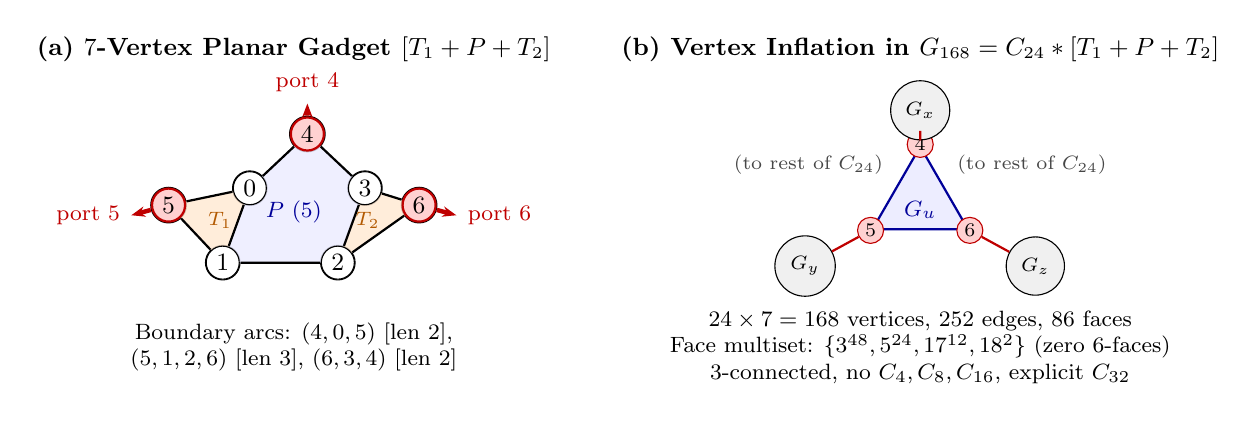
\begin{tikzpicture}[scale=0.86, every node/.style={font=\small}]
  % Left: The 7-vertex planar gadget [T1 + P + T2]
  \begin{scope}[shift={(0,0)}]
    \node[font=\bfseries\small] at (2.15, 4.25) {(a) $7$-Vertex Planar Gadget $[T_1 + P + T_2]$};
    \node[circle, draw, fill=white, inner sep=1.8pt] (v0) at (1.5, 2.2) {$0$};
    \node[circle, draw, fill=white, inner sep=1.8pt] (v1) at (1.1, 1.1) {$1$};
    \node[circle, draw, fill=white, inner sep=1.8pt] (v2) at (2.8, 1.1) {$2$};
    \node[circle, draw, fill=white, inner sep=1.8pt] (v3) at (3.2, 2.2) {$3$};
    \node[circle, draw, fill=red!20, thick, inner sep=1.8pt] (v4) at (2.35, 3.0) {$4$};
    \node[circle, draw, fill=red!20, thick, inner sep=1.8pt] (v5) at (0.3, 1.95) {$5$};
    \node[circle, draw, fill=red!20, thick, inner sep=1.8pt] (v6) at (4.0, 1.95) {$6$};

    \fill[blue!8, opacity=0.8] (v0.center) -- (v4.center) -- (v3.center) -- (v2.center) -- (v1.center) -- cycle;
    \fill[orange!18, opacity=0.8] (v5.center) -- (v0.center) -- (v1.center) -- cycle;
    \fill[orange!18, opacity=0.8] (v6.center) -- (v2.center) -- (v3.center) -- cycle;

    \draw[thick] (v0)--(v4)--(v3)--(v2)--(v1)--(v0);
    \draw[thick] (v5)--(v0) (v5)--(v1);
    \draw[thick] (v6)--(v2) (v6)--(v3);
    \draw[red!75!black, ultra thick, -{Stealth[length=5pt]}] (v4) -- ++(0, 0.45) node[above, font=\footnotesize]{port $4$};
    \draw[red!75!black, ultra thick, -{Stealth[length=5pt]}] (v5) -- ++(-0.55, -0.15) node[left, font=\footnotesize]{port $5$};
    \draw[red!75!black, ultra thick, -{Stealth[length=5pt]}] (v6) -- ++(0.55, -0.15) node[right, font=\footnotesize]{port $6$};

    \foreach \n/\lab in {v0/0, v1/1, v2/2, v3/3}
      \node[circle, draw, fill=white, inner sep=1.6pt] at (\n) {$\lab$};
    \foreach \n/\lab in {v4/4, v5/5, v6/6}
      \node[circle, draw=red!75!black, fill=red!18, thick, inner sep=1.6pt] at (\n) {$\lab$};

    \node[blue!60!black, font=\footnotesize] at (2.15, 1.85) {$P$ ($5$)};
    \node[orange!70!black, font=\scriptsize] at (1.06, 1.72) {$T_1$};
    \node[orange!70!black, font=\scriptsize] at (3.24, 1.72) {$T_2$};
    \node[font=\footnotesize, align=center] at (2.15, -0.15) {Boundary arcs: $(4,0,5)$ [len $2$],\\$(5,1,2,6)$ [len $3$], $(6,3,4)$ [len $2$]};
  \end{scope}

  % Right: Inflation into C24 -> G168
  \begin{scope}[shift={(8.4,0)}]
    \node[font=\bfseries\small] at (3.0, 4.25) {(b) Vertex Inflation in $G_{168} = C_{24} * [T_1+P+T_2]$};
    \node[regular polygon, regular polygon sides=3, draw=blue!60!black, fill=blue!7, thick, minimum size=1.4cm] (g0) at (3.0, 2.0) {};
    \node[font=\footnotesize, blue!60!black] at (3.0, 1.88) {$G_u$};
    \node[circle, draw=red!75!black, fill=red!18, inner sep=1.2pt, font=\scriptsize] (p4) at (g0.corner 1) {$4$};
    \node[circle, draw=red!75!black, fill=red!18, inner sep=1.2pt, font=\scriptsize] (p5) at (g0.corner 2) {$5$};
    \node[circle, draw=red!75!black, fill=red!18, inner sep=1.2pt, font=\scriptsize] (p6) at (g0.corner 3) {$6$};

    \node[circle, draw, fill=gray!12, minimum size=0.65cm, font=\scriptsize] (n1) at (3.0, 3.35) {$G_{x}$};
    \node[circle, draw, fill=gray!12, minimum size=0.65cm, font=\scriptsize] (n2) at (1.3, 1.05) {$G_{y}$};
    \node[circle, draw, fill=gray!12, minimum size=0.65cm, font=\scriptsize] (n3) at (4.7, 1.05) {$G_{z}$};

    \draw[red!75!black, thick] (p4)--(n1) (p5)--(n2) (p6)--(n3);
    \node[gray!55!black, font=\scriptsize] at (1.35, 2.55) {(to rest of $C_{24}$)};
    \node[gray!55!black, font=\scriptsize] at (4.65, 2.55) {(to rest of $C_{24}$)};

    \node[font=\footnotesize, align=center] at (3.0, -0.15) {$24 \times 7 = 168$ vertices, $252$ edges, $86$ faces\\Face multiset: $\{3^{48}, 5^{24}, 17^{12}, 18^{2}\}$ (zero $6$-faces)\\$3$-connected, no $C_4, C_8, C_{16}$, explicit $C_{32}$};
  \end{scope}
\end{tikzpicture}
\caption{Sharpness witness $G_{168} = C_{24} * [T_1 + P + T_2]$ for Theorem~\ref{thm:main1}: (a)~the $7$-vertex planar gadget with external ports $4, 5, 6$; (b)~local incidence at an inflated vertex $G_u$ of the $24$-vertex fullerene $C_{24}$ with its three neighboring gadgets $G_x, G_y, G_z$, achieving exact $3$-connectivity, zero $C_4, C_8, C_{16}$, and an explicit simple $C_{32}$.}\label{fig:g168}
\end{figure}

%% =============================================================================
\section{Main Theorem 2: All Planar Induced Claw-Free Graphs (\texorpdfstring{$\delta \ge 3$}{delta >= 3}) Contain \texorpdfstring{$C_4..C_{64}$}{C4..C64}}\label{sec:clawfree}
%% =============================================================================

We now prove Theorem~\ref{thm:main2} by reducing any $C_4$-free planar induced claw-free graph with $\delta(G) \ge 3$ to a planar cubic skeleton $H$ and lifting dyadic cycles from Theorem~\ref{thm:main1} via a sharp interval-realization lemma.

\begin{lemma}[Claw-Free Bowtie Representation and Planar Bowtie-Splitting]\label{lem:clawfree-split}
Let $G$ be a finite nonempty simple induced claw-free (induced $K_{1,3}$-free) graph with $\delta(G) \ge 3$ and no $C_4$.
\begin{enumerate}[label=(\roman*),leftmargin=2.2em]
  \item Every vertex $v \in V(G)$ has degree $3$ or $4$; its open neighborhood $N_G(v)$ is isomorphic to $K_2 + K_1$ (if $d_G(v) = 3$) or $K_2 + K_2$ (if $d_G(v) = 4$).
  \item Consequently, the triangles of $G$ are edge-disjoint, each degree-$3$ vertex lies in a unique triangle, each degree-$4$ vertex lies in exactly two triangles (forming a \emph{bowtie}), and $G \cong T(H)/B$ for a marked finite nonempty simple cubic skeleton $(H, B)$ ($B \subseteq E(H)$, with at most one edge of $B$ in any triangle of $H$), unique up to isomorphism of marked skeletons, where $T(H)$ is obtained from $H$ by inflating each vertex $u \in V(H)$ into a triangle $T_u$ whose three vertices correspond to the three incident edges of $u$ in $H$, and $T(H)/B$ contracts each inter-triangle edge $e \in B$ to a single degree-$4$ bowtie vertex $x_e$.
  \item \textbf{Planar Bowtie-Splitting:} If $G$ is planar, then both $T(H)$ and the cubic skeleton $H$ are planar.
\end{enumerate}
\end{lemma}

\begin{proof}
(i) Because $G$ is induced $K_{1,3}$-free, the independence number of $N_G(v)$ satisfies $\alpha(N_G(v)) \le 2$. Because $G$ is $C_4$-free, $N_G(v)$ contains no $2$-edge path $a - b - c$ (regardless of whether $ac \in E(G)$, $v - a - b - c - v$ is a simple $4$-cycle in $G$). Hence every connected component of $N_G(v)$ is $K_1$ or $K_2$. With at most two components ($\alpha \le 2$) and $|N_G(v)| = d_G(v) \ge 3$, the only possibilities are $K_2 + K_1$ ($d = 3$) and $K_2 + K_2$ ($d = 4$).

(ii) By~(i), no edge lies in two triangles (else a diamond contains $C_4$). Construct $H$ with one vertex $u$ per triangle $T_u$ of $G$, adding an edge $uv \in E(H) \setminus B$ for each edge of $G$ joining a degree-$3$ vertex of $T_u$ to a degree-$3$ vertex of $T_v$, and adding a bowtie edge $uv \in B$ for each degree-$4$ vertex $x_{uv} \in V(T_u) \cap V(T_v)$. Since every triangle has $3$ vertices, $H$ is $3$-regular and nonempty. Moreover, $H$ is simple: a loop at $u$ is impossible (vertices of $T_u$ have no extra edges inside $T_u$), two parallel physical edges between $T_u$ and $T_v$ form a $C_4$, two parallel bowtie vertices form a diamond (hence $C_4$), and a bowtie vertex $x \in V(T_u) \cap V(T_v)$ together with a physical edge $a_1 b_1$ between $T_u = \{x, a_1, a_2\}$ and $T_v = \{x, b_1, b_2\}$ yields the simple $4$-cycle $x - a_1 - b_1 - b_2 - x$. Similarly, if a triangle $uvw$ of $H$ had two edges $uv, vw \in B$ with bowtie vertices $x_{uv}, x_{vw}$, then letting $c_u \in T_u, c_w \in T_w$ be the endpoints of the third edge $uw$ (whether physical or bowtie), $x_{uv} - x_{vw} - c_w - c_u - x_{uv}$ (if $uw \notin B$) or $x_{uv} - x_{vw} - x_{uw}$ sharing $x_{uv} x_{vw}$ with $T_v$ (if $uw \in B$, forming a diamond hence $C_4$) yields a $C_4$. Hence $(H, B)$ is simple, has $\le 1$ edge of $B$ per triangle, and is uniquely determined up to isomorphism of marked skeletons by the triangle decomposition of $G$.

(iii) Fix a planar embedding of $G$ on $S^2$. At any degree-$4$ bowtie vertex $x_{uv} = T_u \cap T_v$, the two incident edges of $T_u$ must appear \emph{consecutively} in the cyclic rotation around $x_{uv}$: if the edges of $T_u$ alternated with those of $T_v$, then the third edge of $T_v$ would connect the two endpoints of $T_v$ on opposite sides of the Jordan curve $T_u$, forcing a crossing. Splitting $x_{uv}$ locally into two degree-$3$ vertices (separating the two consecutive edges of $T_u$ from those of $T_v$) joined by a short edge inside a small disk around $x_{uv}$ preserves planarity. Performing this split at every degree-$4$ vertex yields a planar embedding of $T(H)$. Finally, contracting each of the pairwise vertex-disjoint triangles $T_u$ ($u \in V(H)$) to a single vertex produces a planar embedding of $H$.
\end{proof}

\begin{lemma}[Simple Cycle Lift-Window and Bowtie-Forest Exclusion]\label{lem:lift-window}
Let $G = T(H)/B$ be a $C_4$-free induced claw-free graph with simple cubic skeleton $H$ and bowtie set $B \subseteq E(H)$, and let $C$ be a simple cycle of length $L \ge 3$ in $H$ containing $k := |E(C) \cap B|$ traversed bowtie edges and $m := |E_{\mathrm{chord}}(C) \cap B|$ internal chordal bowtie edges (edges of $B \setminus E(C)$ with both endpoints on $V(C)$). Then:
\begin{enumerate}[label=(\roman*),leftmargin=2.2em]
  \item \textbf{Exact Realization of the Lift Window:} Every integer $\ell \in [2L - k,\; 3L - k - m]$ is the length of a genuine simple cycle in $G$.
  \item \textbf{Bowtie-Forest Exclusion:} If $m = 0$ and $r := L - k \le 2$, then $[2L - k, 3L - k] = [L + r, 2L + r]$ contains a power of two $2^a \ge 4$ (with $2^a \le 2L + 2$). In particular, if $G$ avoids all dyadic cycles, then $H_B := (V(H), B)$ is an \emph{induced forest} in $H$ ($r = 0, 1$ impossible) and the contraction $H / H_B$ is \emph{simple} ($r = 2$ impossible).
  \item \textbf{Universal Dyadic Transfer:} Whenever $H_B[V(C)]$ is acyclic (a forest on $L$ vertices), we have $k + m \le L - 1$, and therefore both $2L$ and $2L + 1$ lie in $[2L - k, 3L - k - m]$.
\end{enumerate}
\end{lemma}

\begin{proof}
(i) For each vertex $u \in V(C)$, its two incident cycle edges $e_{\mathrm{in}}(u), e_{\mathrm{out}}(u) \in E(C)$ are distinct and therefore correspond to two distinct port vertices $p_{\mathrm{in}}(u), p_{\mathrm{out}}(u) \in V(T_u)$; let $p_{\mathrm{sp}}(u)$ denote the third (\emph{spare}) vertex of $T_u$. Each edge $e \in E(C) \setminus B$ contributes $1$ physical inter-triangle edge of $G$ ($L - k$ edges in total), whereas each edge $e \in E(C) \cap B$ identifies $p_{\mathrm{out}}(u) = p_{\mathrm{in}}(v) = x_e$ ($0$ inter-triangle edges). The $2L$ traversed port occurrences along $C$ are pairwise distinct except for the $k$ exact coincidences along traversed bowtie edges $e \in E(C) \cap B$, yielding $2L - k$ distinct traversed port vertices in $G$ (since $H$ is simple).

Inside each triangle $T_u$ ($u \in V(C)$), we may route from $p_{\mathrm{in}}(u)$ to $p_{\mathrm{out}}(u)$ either via the single edge $p_{\mathrm{in}}(u) p_{\mathrm{out}}(u)$ (length $1$) or via the $2$-edge detour $p_{\mathrm{in}}(u) - p_{\mathrm{sp}}(u) - p_{\mathrm{out}}(u)$ (length $2$, contributing $+1$ to the cycle length). A spare vertex $p_{\mathrm{sp}}(u)$ is never a traversed port of any $T_v$ ($v \in V(C)$), because $p_{\mathrm{sp}}(u)$ corresponds to the unique edge of $H$ at $u$ not in $E(C)$. Distinct spare occurrences $p_{\mathrm{sp}}(u), p_{\mathrm{sp}}(v)$ ($u \neq v \in V(C)$) coincide if and only if $uv \in E_{\mathrm{chord}}(C) \cap B$, forming $m$ pairwise disjoint pairs alongside $L - 2m$ unshared spare vertices. Choosing any subset $S$ of $|S| = s \in \{0, 1, \dots, L - m\}$ spare detours taking at most one detour from each of the $m$ chordal pairs yields a simple cycle in $G$ of exact length $(L - k) + L + s = 2L - k + s \in [2L - k,\; 3L - k - m]$.

(ii) Let $x := L + r \ge 3$ and let $2^a$ be the smallest power of two $\ge x$ (so $a \ge 2$). Then $2^{a-1} \le x - 1$, hence $2^a \le 2(x - 1) = 2L + 2r - 2 \le 2L + r$ whenever $r \le 2$ (proved in Lean~4 as \texttt{bowtie\_forest\_exclusion}). Applying this to: (a)~a shortest all-bowtie cycle in $H_B$ ($r = 0, m = 0$) proves $H_B$ is acyclic; (b)~the unique path in a tree component of $H_B$ closed by a single edge of $H \setminus B$ ($r = 1, m = 0$ by acyclicity) proves $H_B$ is induced; (c)~two edges of $H \setminus B$ joining two distinct tree components of $H_B$ closed by the unique paths (possibly of length $0$ if endpoints coincide) in those two trees ($r = 2, m = 0$) proves at most one edge joins any two tree components, so $H/H_B$ is simple.

(iii) A forest on $L$ vertices has at most $L - 1$ edges (\texttt{forest\_edge\_bound\_on\_cycle}), so $k + m = |E(H_B[V(C)])| \le L - 1$, giving $2L - k \le 2L < 2L + 1 \le 3L - k - m$ (\texttt{universal\_bowtie\_transfer}).
\end{proof}

\begin{proof}[Proof of Theorem~\ref{thm:main2}]
Let $G$ be a finite nonempty simple planar induced claw-free graph with $\delta(G) \ge 3$. If $G$ contains a $C_4$, we are done. Otherwise, by Lemma~\ref{lem:clawfree-split}, $G \cong T(H)/B$ for a finite nonempty simple cubic planar graph $H$ and bowtie set $B \subseteq E(H)$. By Theorem~\ref{thm:main1}, $H$ contains a simple cycle $C$ of length $L \in \{4, 8, 16, 32\}$. Consider the induced bowtie subgraph $H_B[V(C)]$:
\begin{itemize}[leftmargin=1.8em]
  \item If $H_B[V(C)]$ contains a cycle, let $C'$ be a shortest cycle in $H_B[V(C)]$, of length $3 \le L' \le L \le 32$. Then $C'$ has $k' = L'$ ($r' = 0$) and $m' = 0$ (by minimality of $L'$), so by Lemma~\ref{lem:lift-window}(i)--(ii), $G$ contains a simple cycle of length $2^a \in [L', 2L'] \cap [4, 64]$.
  \item Otherwise $H_B[V(C)]$ is a forest on $L$ vertices, so $k + m \le L - 1$. By Lemma~\ref{lem:lift-window}(i) and~(iii) (\texttt{dyadic\_cycle\_lift\_window}), $G$ contains a simple cycle of length $2L \in \{8, 16, 32, 64\}$. \qedhere
\end{itemize}
\end{proof}

%% =============================================================================
\section{Main Theorem 3: General Planar (\texorpdfstring{$\delta \ge 3$}{delta >= 3}) \texorpdfstring{$C_{16}$}{C16} Trilogy}\label{sec:trilogy}
%% =============================================================================

Fix a forbidden cycle length $g_{\mathrm{forb}} \in \{3, 5, 6\}$, and suppose for contradiction that $G$ is an edge-minimal counterexample to Theorem~\ref{thm:main3} among finite nonempty simple planar graphs with $\delta(G) \ge 3$ avoiding $\{C_4, C_8, C_{16}, C_{g_{\mathrm{forb}}}\}$. By Lemma~\ref{lem:general-cap}, $\Vge(G)$ is an independent set, and there exists a $3$-connected plane graph $H^+$ ($\delta(H^+) \ge 3$) with at most two frozen faces $\Ffrz(H^+) \subseteq \{f_1, f_2\}$ sharing the cap edge $ab$ such that: every cycle avoiding $ab$ avoids $\{C_4, C_8, C_{16}, C_{g_{\mathrm{forb}}}\}$, and no clean edge joins two vertices of $\Vge(H^+)$.

Assign Euler vertex-face initial charges
\[
  \chz(v) := 6 - 2 d_{H^+}(v) \quad (v \in V(H^+)), \qquad
  \chz(f) := 6 - d(f) \quad (f \in F(H^+)),
\]
so that $\sum_v \chz(v) + \sum_f \chz(f) = 12$ by~\eqref{eq:euler-vf}. Note that $\chz(v) = 0$ for cubic vertices ($d = 3$) and $\chz(v) = 6 - 2k \le -2$ for high-degree vertices ($d = k \ge 4$), allowing every $v \in \Vge(H^+)$ to act as a charge sink (Figure~\ref{fig:discharging}(b)).

\begin{lemma}[Soundness and Seed Completeness of Noncrossing Outer-Rim Partition Enumeration]\label{lem:rim-sound}
Let $\mathcal{P} = (F_1, \dots, F_m)$ be an abstract planar $2$-complex forming a closed topological disk $D_{\mathrm{abs}}$ bounded by a simple outer-rim cycle $R = (r_0, r_1, \dots, r_{q-1})$, mapped into $S^2$ by the realization $\Phi : D_{\mathrm{abs}} \to S^2$ of $m$ distinct clean faces of $3$-connected $H^+$ such that open faces map homeomorphically onto disjoint open faces of $H^+$, interior edges map injectively onto their prescribed shared edges, and every interior vertex of $D_{\mathrm{abs}}$ is mapped injectively and disjointly from $\Phi(R)$. Then:
\begin{enumerate}[label=(\roman*),leftmargin=2.2em]
  \item \textbf{Noncrossing Exterior-Disk Partition:} The equivalence relation on $\{0, \dots, q-1\}$ induced by $\Phi(r_i) = \Phi(r_j)$ is a \emph{noncrossing partition} of the cyclic sequence $R$.
  \item \textbf{Validity Filters:} The realized quotient $\Phi(\mathcal{P})$ satisfies: (a)~every face is simple, (b)~any two distinct faces share at most one edge (Lemma~\ref{lem:plane-basics}(ii)), (c)~no two vertices of degree $\ge 4$ in the edge union of $\Phi(\mathcal{P})$ are adjacent along any clean edge (since patch degree lower-bounds ambient degree in $H^+$ and $\Vge(H^+)$ is independent on clean edges by Lemma~\ref{lem:general-cap}(ii)(b)), and (d)~the edge union of $\Phi(\mathcal{P})$ contains no cycle in $\{C_4, C_8, C_{16}, C_{g_{\mathrm{forb}}}\}$.
  \item \textbf{Seed Completeness:} For every seed class in \texttt{cert/verify\_planar\_eg.py} (Sections~\ref{subsec:c3free}--\ref{subsec:c6free}), the omitted/fixed rim vertices and contact tests in \texttt{rim\_quotients} and \texttt{check\_cor\_attach} omit zero valid surviving quotients; hence if every valid emitted quotient fails \texttt{patch\_status}, then $\mathcal{P}$ cannot occur on clean faces of $H^+$.
\end{enumerate}
\end{lemma}

\begin{proof}
(i) Choose a slightly shrunken concentric closed disk $D' \subset \mathrm{int}(D_{\mathrm{abs}})$ whose boundary $\Gamma' := \partial D'$ stays strictly inside $\mathrm{int}(D_{\mathrm{abs}})$ (crossing each interior edge incident to $R$ once just before its rim endpoint). Because $\Phi$ is injective on $\mathrm{int}(D_{\mathrm{abs}})$, the image $\Phi(\Gamma')$ is a genuine simple closed Jordan curve on $S^2$. By the Jordan--Schoenflies theorem, $S^2 \setminus \Phi(\Gamma')$ consists of two open topological disks: the interior disk $U_{\mathrm{in}} := \Phi(\mathrm{int}(D'))$ and the exterior open disk $U_{\mathrm{out}} := S^2 \setminus \Phi(D')$. For each $k \in \{0, \dots, q-1\}$, draw a short radial arc $\gamma_k \subset D_{\mathrm{abs}} \setminus \mathrm{int}(D')$ inside the face corner(s) incident to $r_k$ from a point $p_k \in \Gamma'$ (in cyclic order $p_0, \dots, p_{q-1}$ around $\Gamma'$) to $r_k$, so that the images $\Phi(\gamma_k \setminus \{p_k, r_k\})$ are pairwise disjoint open arcs in $U_{\mathrm{out}}$. If four indices $i_1 < j_1 < i_2 < j_2$ in cyclic order satisfied $\Phi(r_{i_1}) = \Phi(r_{i_2}) = u$ and $\Phi(r_{j_1}) = \Phi(r_{j_2}) = v$ with $u \neq v$, then $\Phi(\gamma_{i_1}) \cup \Phi(\gamma_{i_2})$ and $\Phi(\gamma_{j_1}) \cup \Phi(\gamma_{j_2})$ would be two disjoint simple arcs inside the closed exterior disk $\overline{U_{\mathrm{out}}}$ connecting alternating boundary pairs $(p_{i_1}, p_{i_2})$ and $(p_{j_1}, p_{j_2})$ on $\partial U_{\mathrm{out}} = \Phi(\Gamma')$, contradicting the Jordan curve theorem.

(ii) Conditions (a)--(d) hold in $H^+ - ab \subseteq G$ by Lemma~\ref{lem:plane-basics}(i)--(ii) and Lemma~\ref{lem:general-cap}(ii), because every edge of $\Phi(\mathcal{P})$ is a clean edge and patch vertex degrees lower-bound ambient degrees in $H^+$.

(iii) In \texttt{rim\_quotients}, the exact noncrossing interval guard (\texttt{peer[0] < last < peer[-1]}) and hereditary pairwise face-contact guard (\texttt{compatible\_with\_contacts}, which checks only that identifying two rim vertices never forces two faces to share $\ge 3$ vertices or $2$ non-adjacent vertices) preserve every valid quotient. In every seed below, each shared interior edge maps injectively by facial contact hypotheses (Lemma~\ref{lem:plane-basics}(ii)), and when repeated rim incidence is already prescribed in the seed (e.g.\ \texttt{f7\_pair\_k} at vertex $1$, \texttt{v9} at vertex $0$, or \texttt{3-hex+2T} at vertex $0$), the noncrossing corner-arc proof of~(i) applies directly to the cut-open cyclic rim sequence with the fixed vertex excluded (since its incident wedges form a contiguous sector on $\partial U_{\mathrm{out}}$). We justify interior-vertex injectivity and every omitted/fixed label across all seed classes:
\begin{itemize}[leftmargin=1.5em]
  \item \emph{All-interior-faces-present seeds} ($C_3$-free \texttt{enum\_ring}, $C_5$-free \texttt{4-hex}, \texttt{5-hex+2v}, \texttt{k4t2}, \texttt{f7\_3h}, and all $9$ $C_6$-free seeds): Every interior vertex has its full ambient degree already saturated by its incident faces inside $\mathcal{P}$ (either cubic with all $3$ faces present, or degree $4$/$5$ with all $4$/$5$ faces present in \texttt{4-hex}, \texttt{5-hex+2v}, \texttt{k4t2}), so its closed local wedge fan leaves zero free wedges and it cannot coincide with any other vertex of $\mathcal{P}$.
  \item \emph{Corannulene extensions} (\texttt{check\_cor\_attach}, \texttt{verify\_planar\_eg.py:1628--1656}): By \texttt{enum\_ring((6,6,6,6,6))} ($46 \to 1$ survivor), the $15$-rim Corannulene is uniquely unidentified. Hence in \texttt{(*cor, new\_face)}, no two vertices of \texttt{cor} coincide and no two vertices of \texttt{new\_face} coincide, so every identification is a partial bijection between \texttt{new\_vs} and the remaining rim vertices of \texttt{cor}. By~(i), traversing \texttt{new\_vs} clockwise and the Corannulene rim counterclockwise (\texttt{arc\_rev}), the bijection must be order-preserving. Vertices of $H_0$ (in the $+P$ cases) and of $H_0 \cup H_4$ (in the valley cases, leaving \texttt{v\_arc\_rev}$=[17,16,8,15,14,7,13,12]$) are excluded from \texttt{arc\_rev} because \texttt{new\_face} already shares an edge with $H_0$ (and $H_4$) and cannot share a third vertex with them by Lemma~\ref{lem:plane-basics}(ii).
  \item \emph{$C_5$-free \texttt{v9} (fixed vertex $0$), \texttt{3-hex+2T} (fixed vertex $0$), and \texttt{f7\_pair\_k} (fixed vertex $1$):} In \texttt{f7\_pair\_k} (\texttt{lines 1776--1784}), vertex $1$ belongs to $F_7, H_1, H_2$, so by face simplicity and Lemma~\ref{lem:plane-basics}(ii) it cannot identify with any vertex of $F_7, H_1, H_2$ or either triangle apex $30, 31$ ($0$ extra quotients when included); skipping \texttt{len(set(q[1]) \& set(q[2])) == 2} excludes only the adjacent-hexagon case already covered by \texttt{f7\_3h}. In \texttt{3-hex+2T} (\texttt{lines 1760--1771}), vertex $0$ has $d(0) \ge 4$ (so $H_1$ and $H_3$ cannot share an edge, enforced by \texttt{len(set(q[0]) \& set(q[2])) < 2}) and lies on all three hexagons, preventing identification with any vertex of $H_1 \cup H_2 \cup H_3$ or either triangle apex ($C_4$/$C_5$). In \texttt{v9} (\texttt{lines 1724--1752}), vertex $0$ lies on $H_1$ and $H_2$, and every noncrossing identification of $0$ with a remaining rim vertex violates \texttt{patch\_status} ($C_4, C_5$, double contact, or adjacent high vertices; direct verification confirms $0$ extra valid quotients across all $25$ \texttt{v9} seeds when $0$ is included).
  \item \emph{$C_5$-free \texttt{aux10} and \texttt{H6} (\texttt{lines 1817--1854}):} Every vertex of \texttt{rim10} is fixed because each triangle and \texttt{aux}/\texttt{h6} already shares an edge with $F_{10}$ and cannot share a third vertex with $F_{10}$ (Lemma~\ref{lem:plane-basics}(ii)). In \texttt{aux10}, omitting $(21, 29)$ holds whenever $T_1, T_9$ have cubic apices (all $3$ edges at $21, 29$ are already present in the patch); if $21$ or $29$ has degree $\ge 4$, the corresponding triangle is already non-cubic (sending $\le 2/3$ to $F_{10}$; moreover, even including $21, 29$ in \texttt{ext} yields only $3$ additional valid---and killed---quotients alongside $1{,}187$ invalid ones, with zero survivors).
  \item \emph{$C_5$-free clean $T_{\mathrm{frz}} + H_6 + T'$ (\texttt{lines 1785--1788}):} Here $T_{\mathrm{frz}} = (0, 1, 2)$ is a clean triangle (avoiding $ab$, with both frozen faces sharing edges $(0, 1)$ and $(0, 2)$ at the cubic cap endpoint $0$), $H_6 = (2, 1, 3, 4, 5, 6)$ is a clean $6$-face sharing edge $(1, 2)$, and $T' = (v, u, 7)$ is a clean triangle on one of the $5$ remaining edges $uv \in \{(3,4),(4,5),(5,6),(6,2),(1,3)\}$ of $H_6$. In the unmerged $3$-face model, each of the $5$ placements contains an explicit clean $C_4$ or $C_8$ avoiding $ab$. Could two distinct vertices $x \neq y$ of that $C_4$ or $C_8$ coincide in $H^+$? Any such identification must pair vertex $0$ or vertex $7$ with a vertex not sharing a face with it (since faces are simple and share at most one edge by Lemma~\ref{lem:plane-basics}(ii)): (a)~identifying $0 = 7$ creates either a double vertex contact of $T_{\mathrm{frz}}$ with $T'$ or a clean $C_4$ ($0\text{--}1\text{--}3\text{--}0$ or $0\text{--}2\text{--}6\text{--}0$) or clean $C_5$ ($0\text{--}1\text{--}3\text{--}4\text{--}0$ or $0\text{--}2\text{--}6\text{--}5\text{--}0$); (b)~identifying $0 \in \{3, 4, 5, 6\}$ gives $T_{\mathrm{frz}}$ and $H_6$ a third common vertex, violating Lemma~\ref{lem:plane-basics}(ii); and (c)~identifying $7 \in \{1, 2, 3, 4, 5, 6\} \setminus \{u, v\}$ gives $T'$ and $H_6$ a third common vertex, again violating Lemma~\ref{lem:plane-basics}(ii). Thus all $5$ explicit $C_4/C_8$ cycles lift simply to $H^+ - ab$. \qedhere
\end{itemize}
\end{proof}

\subsection{Part (a): All \texorpdfstring{$C_3$}{C3}-Free General Planar Graphs (\texorpdfstring{$\delta \ge 3$}{delta >= 3})}\label{subsec:c3free}

Clean faces have degrees in $\{5, 6, 7, 9, 10, 11, \dots\}$; only clean $5$-faces ($\chz = +1$) are positive, and no two clean $5$-faces share an edge ($C_8$). Fix a canonical total ordering $\prec$ on $V(H^+) \cup E(H^+) \cup F(H^+)$.
\begin{itemize}[leftmargin=1.8em]
  \item \textbf{Rule V1 (High-Degree Absorption):} Every clean $5$-face incident to at least one vertex in $\Vge(H^+)$ sends $+1$ to its $\prec$-first such vertex. Every remaining \emph{pure cubic} clean $5$-face $P$ has all $5$ vertices of degree $3$, so pure cubic $5$-faces are pairwise vertex-disjoint (sharing a cubic vertex would force sharing an edge, giving $C_8$).
  \item \textbf{Rule P1 (Complete Ring Classification for Pure Cubic $P$):} Partition all pure cubic $5$-faces $P$ into three exhaustive cases: (1)~if $P$ touches at least one frozen face or clean $\ge 10$-face, send $+1$ to the $\prec$-first such face; (2)~else all $5$ neighbors of $P$ are clean in $\{6, 7, 9\}$: if at least two lie in $\{7, 9\}$, send $1/2$ to each of the $\prec$-first two (bounded by $w_P(7) = 1/2$ and $w_P(9) = 3/4$); (3)~otherwise at least four neighbors are clean $6$-faces, leaving exactly three rings: $(6,6,6,6,7)$ ($59 \to 0$ survivors), $(6,6,6,6,9)$ ($105 \to 0$ survivors), and $(6,6,6,6,6)$ ($46 \to 1$ survivor, the unique unidentified $15$-rim \emph{Corannulene}), all certified by Lemma~\ref{lem:rim-sound}.
  \item \textbf{Rule C1 (Corannulene Spoke / Valley Discharge):} By Lemma~\ref{lem:rim-sound} (\texttt{check\_cor\_attach}), attaching a clean $5$-face $P'$ to either outer edge type of a Corannulene hexagon yields $106 \to 0$ survivors. Consequently: (a)~no clean $6$-face belongs to two distinct Corannulenes (else the second Corannulene's $5$-face would attach along an outer edge of that $6$-face), so distinct Corannulenes incident to a spoke vertex $v \in \Vge(H^+)$ occupy \emph{pairwise disjoint pairs of $6$-face wedges} at $v$; and (b)~no pure cubic $5$-face is adjacent to a Corannulene valley edge. If any of the $5$ spoke vertices $a_0,\dots,a_4$ of a Corannulene lies in $\Vge(H^+)$, $P$ sends $+1$ to the $\prec$-first such spoke vertex; at any $v$ of degree $k \ge 4$ receiving from $c$ Corannulenes (consuming $2c$ disjoint $6$-face wedges) and non-adjacent clean $5$-faces in the remaining $k - 2c$ wedges,
  \[
    \chf(v) \;\le\; 6 - 2k + \left\lfloor \frac{k - 2c + 1}{2} \right\rfloor + c \;=\; 6 - 2k + \left\lfloor \frac{k + 1}{2} \right\rfloor \;\le\; 0 \qquad (\forall k \ge 4,\ 2c \le k),
  \]
  kernel-proved in \texttt{c3free\_vertex\_absorption}. Otherwise all $5$ spoke vertices are cubic, and \texttt{check\_cor\_attach} kills all $5$ valley degrees $d \in \{5, 6, 7, 9, 10\}$ ($990 \to 0$ survivors; $1{,}260 = 59 + 105 + 106 + 990$ total $C_3$-free rim kills), so every valley is frozen or clean $\ge 11$ and receives $+1/5$ from $P$.
  \item \textbf{Graph-to-Token Map and Clean/Frozen Tally:} Around any clean $d$-face $F_d$ ($d \ge 6$), each boundary edge is encoded as $P$ (width $1$, weight $w_P(d) \in \{0, 1/2, 3/4, 1\}$), $V$ (width $2$, weight $1/5$ for $d \ge 11$, covering the two consecutive Corannulene $6$-face edges at a valley), or $N$ (width $1$, weight $0$). No two $P$ tokens are adjacent ($C_8$), and no $P$ is adjacent to $V$ (by the $106$ \texttt{Cor+P} kills). Because pure cubic $5$-faces are pairwise vertex-disjoint and each gives a $+3$ detour avoiding $V(F_d)$ (Lemma~\ref{lem:plane-basics}(ii)), $m$ such $5$-faces on $F_d$ yield simple cycles of lengths $d + 3j$ ($0 \le j \le m$), bounding the count of $P$ by \texttt{max\_p}. Exact cyclic DP (\texttt{c3free\_clean\_small\_bounds}) verifies $\chf(f) \le 0$ for clean $d \in \{6, 7, 9..13\}$; for clean $d \ge 14$, the packed Bellman--Ford bound (\texttt{c3free\_clean\_d\_ge\_14\_bound}, slope $11/20$) gives $\chf(f) \le 6 - d + \frac{11}{20} d \le 0$. Around any frozen face $f_i$ ($d \ge 3$), breaking at $ab$ produces a length-$(d-1)$ path in $\{N, P, V\}$ (with $w_P = 1, w_V = 1/5$ and no adjacent $PP, PV, VP$). If the path contains $p$ $P$-tokens and $v$ $V$-tokens, then for $p \ge 1$ the $p$ $P$-tokens require at least $p - 1$ separating $N$-tokens (since $P$ cannot touch $P$ or $V$), so $L = d - 1 \ge 2p - 1 + 2v \implies p + v/5 \le p + v \le \lfloor d/2 \rfloor$ (and for $p = 0$, $L = d - 1 \ge 2v \implies v/5 \le v \le \lfloor (d-1)/2 \rfloor \le \lfloor d/2 \rfloor$). This unbounded symbolic counting bound (also cross-checked finitely for $d \le 24$ in Python and via the Bellman--Ford slope-$1/2$ potential in \texttt{c3free\_frozen\_cap\_bound}) gives $\chf(f_i) \le (6 - d) + \lfloor d/2 \rfloor \le 4$ for all $d \ge 3$ and $\chf(f_1) + \chf(f_2) \le 8 < 12$, contradicting~\eqref{eq:euler-vf}.
\end{itemize}

\subsection{Part (b): All \texorpdfstring{$C_5$}{C5}-Free General Planar Graphs (\texorpdfstring{$\delta \ge 3$}{delta >= 3}, Zero \texorpdfstring{$R_{10}$}{R10})}\label{subsec:c5free}

Clean faces have degrees in $\{3, 6, 7, 9, 10, 11, \dots\}$; only clean $3$-faces ($\chz = +3$) are positive. Because $\Vge(H^+)$ is independent on clean edges, every clean $3$-face contains at most one vertex in $\Vge(H^+)$, cannot touch any clean $\{3, 4, 5, 7, 8, 15\}$-face, and every clean $6$-face touches at most one clean $3$-face ($6+2=8$).

\begin{itemize}[leftmargin=1.8em]
  \item \textbf{Vertex Absorption (Rules V3/V6) and Wedge Bounds:} Every clean $3$-face incident to $v \in \Vge(H^+)$ sends $+1$ to $v$ if $d(v) = 4$ and $+2$ to $v$ if $d(v) \ge 5$. For charged clean $6$-faces $H_6$ ($c(H_6) \le 1$), \emph{Rule~V6} applies with \emph{non-valley priority}: if $H_6$ has a \emph{non-valley} outer vertex $w \in \Vge(H^+)$ (i.e.\ $w \notin V(T)$ and $w$ is not shared with a second clean $6$-face on the same charging triangle $T$), then $H_6$ sends $c(H_6)$ to its $\prec$-first non-valley outer high vertex $w$; otherwise, if $H_6$ has a \emph{valley} outer vertex $w \in \Vge(H^+)$ (shared with a second clean $6$-face $H_6'$ on $T$), then $H_6$ sends $\min(c(H_6), 1/2)$ to $w$ (preserving and strictly improving the $1/2 + 1/2 = 1$ valley-pair wedge ceiling at $w$, because whenever one of $(H_6, H_6')$ instead discharges to a non-valley outer high vertex, the other still sends at most $1/2$ to $w$). Around $v$ of degree $k \ge 4$ with $t$ incident clean $3$-faces and $h$ outer-charged clean $6$-faces: clean $3$-faces are non-adjacent ($C_4$), and the two wedges immediately flanking any clean $3$-face $T$ at $v$ cannot send Rule-V6 charge to $v$ (since $v \in V(T)$ is not an outer vertex of those faces). Moreover, for any three consecutive clean $6$-faces $H_1, H_2, H_3$ around $v \in \Vge(H^+)$, their shared spoke vertices $2, 3$ are adjacent to $v$ and therefore cubic ($\Vge$-independence), so any charging triangle on an inner spoke edge $(12, 2)/(2, 13)$ or $(15, 3)/(3, 16)$ is necessarily a shared valley triangle; across all $21$ non-valley placements of two distinct charging triangles on any two of $(H_1, H_2, H_3)$, noncrossing outer-rim enumeration (\texttt{3-hex+2T}, \texttt{verify\_planar\_eg.py:1760--1771}, $47$ killed quotients, $0$ survivors, kernel-verified in \texttt{c5VAbsWelds}) eliminates every non-valley pair. Hence:
  \begin{itemize}[leftmargin=1.5em]
    \item $k = 4$ ($\chz = -2$): $t = 2 \implies h = 0$, $\mathrm{in} = 2$; $t = 1 \implies h \le 1$, $\mathrm{in} \le 1 + 1 = 2$; $t = 0 \implies h \le 3$ (since $4$ clean $6$-faces around $v$ are killed by \texttt{4-hex}), and if $h = 3$ then by \texttt{3-hex+2T} at least two adjacent hexagons among $(H_1, H_2, H_3)$ must share a valley triangle (contributing $1/2 + 1/2 = 1$ together, plus at most $1$ from the third hexagon), giving $\mathrm{in} \le 2$.
    \item $k = 5$ ($\chz = -4$): $t = 2 \implies h = 0$, $\mathrm{in} = 4$; $t = 1 \implies h \le 2$, $\mathrm{in} \le 2 + 2 = 4$; $t = 0$: if $h \le 4$ then $\mathrm{in} \le 4$; and $h = 5$ is completely impossible, because $0$ valley triangles violate \texttt{3-hex+2T} on $(H_1, H_2, H_3)$, $1$ valley triangle (say on $(H_1, H_2)$) leaves $(H_3, H_4, H_5)$ valley-free violating \texttt{3-hex+2T}, and $\ge 2$ valley triangles must be non-adjacent (as each $6$-face touches $\le 1$ triangle) and are eliminated by \texttt{5-hex+2v}.
    \item $k \ge 6$ ($\chz = 6 - 2k$): if $t = 0$, $\mathrm{in} \le k \le 2k - 6$; if $t = k/2$, $h = 0$ and $\mathrm{in} = k \le 2k - 6$; if $1 \le t < k/2$, at least $t + 1$ wedges flank the $t$ triangles, so $h \le k - 2t - 1$ and $\mathrm{in} \le 2t + h \le k - 1 < 2k - 6$.
  \end{itemize}
  Thus $\chf(v) \le 0$ for every $v \in \Vge(H^+)$. At a $(k=4, t=2)$ vertex $v = 0$, the two clean triangles $T_1 = (0, 1, 2)$ and $T_2 = (0, 3, 4)$ alternate in cyclic rotation order with the two flanking wedges $F_a$ (between $02$ and $03$) and $F_b$ (between $04$ and $01$); the two \texttt{k4t2} seeds (\texttt{verify\_planar\_eg.py:1758--1759}, giving $51 = 4 + 47$ total vertex-absorption rim kills in \texttt{c5VAbsWelds}) exclude both $F_a = F_b = 9$ and $F_a = F_{\mathrm{opp}}(T_1) = 9$ (encoded as vertex type \texttt{4m}, vs.\ \texttt{4s} for $k=4, t=1$ and \texttt{3} for cubic).

  \item \textbf{Complete Mutually Exclusive Stage-1 and Stage-3 Routing (Zero $R_{10}$):} Note first that at any cubic vertex incident to a clean triangle $T$, two clean $9$-faces cannot meet ($9+9-2=16$), a clean $9$- and $10$-face cannot meet ($3+9+10-6=16$), and a clean $6$-face cannot touch a clean $12$-face ($6+12-2=16$) or $13$-face ($3+6+13-6=16$). Every clean triangle $T$ falls into one of the following mutually exclusive, exact charge-conserving branches (all matched edge-by-edge to \texttt{verify\_planar\_eg.py:1853--2000}):
  \begin{enumerate}[label=(\roman*),leftmargin=2.0em]
    \item \emph{Pure cubic $T$ ($+3$):}
      (a)~Two frozen neighbors ($f_1, f_2, Z$; token $T_{\mathrm{frz}}$): send $(3/2, 3/2, 0)$ (and $T_{\mathrm{frz}}$ cannot be followed by a charged $6$-face by the $5$ direct $T_{\mathrm{frz}} + H_6 + T'$ kills at $\{C_4, C_8\}$).
      (b)~Three clean $6$-faces $(6, 6, 6)$: send $(1, 1, 1)$ to the three $6$-faces (each with an outer high vertex uses Rule~V6; pure cubic Mini-Corannulene routes across its valleys/opposite faces as in Stage~3(H3)).
      (c)~Two clean $6$-faces $(H_L, H_R, X)$ (token $T_{2,L,R}$ on $X$, where $L, R \in \{\texttt{3}, \texttt{4s}, \texttt{4m}\}$ are the outer endpoints of $H_L, H_R$ on $X$): whenever $L$ (resp.\ $R$) is high, $L$ (resp.\ $R$) is an outer high vertex of $H_L$ (resp.\ $H_R$) absorbing up to $+1$ by Rule~V6! Send $(1, 1, 1)$ if $X = 9$; if $X = 10$ or $X \in \{14\} \cup [17,\infty) \cup \Ffrz$, send $(1/2, 1/2, 2)$ when $(L, R) = (\texttt{3}, \texttt{3})$, $(1, 1/2, 3/2)$ when $L$ alone is high (symmetric for $R$), and $(1, 1, 1)$ (for $X=10$) or $(5/6, 5/6, 4/3)$ (for $X \ge 14/\Ffrz$) when both $L, R$ are high; if $X = 11$, send $(0, 0, 3)$ when $(L, R) = (\texttt{3}, \texttt{3})$, $(3/4, 0, 9/4)$ when $L$ alone is high, and $(5/6, 5/6, 4/3)$ when both $L, R$ are high.
      (d)~One clean $6$-face $(6, X, Y)$ (token $T_{1,L/R}$ on $X, Y$): define $w_1(9) = 3/4, w_1(10) = 1, w_1(\ge 11/\Ffrz) = 3/2$; if $X = 11$ (choosing $\prec$-first if both are $11$), send $0$ to $6$, $w_1(Y)$ to $Y$, and $3 - w_1(Y) \le 9/4$ to $X$; else send $w_1(X), w_1(Y)$ to $X, Y$ and $3 - w_1(X) - w_1(Y) \in \{0, 1/2, 3/4, 1\}$ to $6$.
      (e)~Zero clean $6$-faces $(X, Y, Z)$ (token $T$): send $(2/3, 7/6, 7/6)$ on $(9, \ge 11/\Ffrz, \ge 11/\Ffrz)$ and on $(10, \ge 11/\Ffrz, \ge 11/\Ffrz)$; $(11/12, 11/12, 7/6)$ on $(10, 10, \ge 11/\Ffrz)$; and $(1, 1, 1)$ on $(10, 10, 10)$ or $(\ge 11/\Ffrz)^3$ (\texttt{c5free\_budget\_identities}).
    \item \emph{Non-cubic $T$ at $v \in \Vge$ ($+2$ left if $k = 4$; $+1$ left if $k \ge 5$; ordered $(F_{\mathrm{opp}}, F_a, F_b)$ with $F_a, F_b$ at $v$):} Observe first that no special two-frozen branch is needed: if a clean non-cubic $T$ touches both frozen faces $f_1, f_2$, then $f_1, f_2, T$ cannot close around the high vertex $v$ (forcing $d(v) = 3$), so the cap endpoint in $V(T)$ is cubic and one of $\{f_1, f_2\}$ is $F_{\mathrm{opp}}$ while the other is $F_a$ or $F_b$, covered directly by the general rules below (with $w_T(\Ffrz) = 7/6, w_{Ts}(\Ffrz) = 2/3, w_{T1}(\Ffrz) = 3/2, w_{Ts6}(\Ffrz) = 5/4$).
      \begin{itemize}[leftmargin=1.4em]
        \item \emph{Exact $T_{s6}$ caps:} Whenever $F_{\mathrm{opp}} = 6$ and $F_i \neq 6$ ($i \in \{a, b\}$), let $L_i \in \{\texttt{3}, \texttt{4s}, \texttt{4m}\}$ be the outer endpoint of the shared edge between $F_{\mathrm{opp}}$ and $F_i$ (if $L_i \neq \texttt{3}$, then $L_i$ is a \emph{non-valley} outer high vertex of $F_{\mathrm{opp}}$ absorbing up to $+1$ via Rule~V6). Define the exact token cap
        \[
          c_i^{\max} \;:=\; \begin{cases}
            w_{Ts6,3}(F_i) & \text{if } L_i = \texttt{3}\quad\bigl(3/4\text{ for }9,\; 1\text{ for }10,\; 5/4\text{ for }\ge 11/\Ffrz\bigr),\\[2pt]
            w_{Ts,v}(F_i) & \text{if } L_i \neq \texttt{3}\quad\bigl(1/2\text{ if }F_i = 9\text{ and }v = \texttt{4m},\;\text{else }2/3\bigr).
          \end{cases}
        \]
        \item \emph{$k \ge 5$ ($+1$ left):} If at least two neighbors of $T$ are not clean $6$-faces, allocate $+1$ deterministically in $\prec$-order across the non-$6$ neighbors up to their token caps ($w_T \ge 2/3$, $w_{T1} \ge 3/4$, $w_{Ts} \ge 1/2$, $c_i^{\max} \ge 1/2$), so every clean $6$-face receives $0$. If $F_{\mathrm{opp}} \neq 6$ and $F_a = F_b = 6$, send $+1 \le w_{T2}(F_{\mathrm{opp}}, L, R)$ to $F_{\mathrm{opp}}$ and $0$ to $F_a, F_b$. If $F_{\mathrm{opp}} = F_a = 6$ and $F_b \neq 6$ (symmetric for $F_b = 6$), send $c_b := \min(1, c_b^{\max})$ to $F_b$, $1 - c_b \le 1/2$ to $F_{\mathrm{opp}}$, and $0$ to $F_a$ (if $L_b \neq \texttt{3}$, $L_b$ absorbs $1 - c_b \le 1/2$ via Rule~V6; if $L_b = \texttt{3}$, $1 - c_b \le 1/4$ is absorbed via Rule~V6 or Stage~3 by the universal $(T, H_6, X=6)$ capacity bound $\ge 1/2$ below). If $F_{\mathrm{opp}} = F_a = F_b = 6$, send $(1, 0, 0)$ to $(F_{\mathrm{opp}}, F_a, F_b)$ (covered by the non-cubic Mini-Corannulene Stage-3 capacity $\ge 1$ on $F_{\mathrm{opp}}$ below).
        \item \emph{$k = 4$ ($+2$ left), $0$ clean $6$-faces:} Note that if $F_{\mathrm{opp}} = 9$, then at the two cubic endpoints of $F_{\mathrm{opp}}$ both $F_a, F_b$ are $\ge 11/\Ffrz$ ($9+9-2=16$, $3+9+10-6=16$), so $(2/3, 2/3, 2/3)$ already balances $+2$ within $(w_T(9) = 2/3, w_{Ts}(\ge 11) = 2/3, 2/3)$. Exhaustively: send $(1, 1/2, 1/2)$ if $F_a = F_b = 9$ (only at \texttt{4s}); $(5/6, 1/2, 2/3)$ if $\{F_a, F_b\} = \{9, \ge 10/\Ffrz\}$ (since $F_{\mathrm{opp}} \ge 11/\Ffrz$); and $(2/3, 2/3, 2/3)$ in all remaining cases (including $F_{\mathrm{opp}} = 9$ and all $\ge 10/\Ffrz$). Every triple sums to $2$ and sends $\le 2/3$ to every clean $10$-face.
        \item \emph{$k = 4$ ($+2$ left), $\ge 1$ clean $6$-face:} Order the two wedges at $v$ with $F_a \prec F_b$; every branch below is exact, capacity-respecting, and verified against Stage-3 noncrossing outer-rim exclusions in \texttt{cert/verify\_parity\_and\_dp.py}:
          (1)~\emph{$F_{\mathrm{opp}} = 6$ and $F_a, F_b \neq 6$:} Set
          \[
            c_a \;:=\; \min(2,\; c_a^{\max}), \qquad c_b \;:=\; \min(2 - c_a,\; c_b^{\max}), \qquad c_{\mathrm{opp}} \;:=\; 2 - c_a - c_b \;\ge\; 0.
          \]
          If $L_a \neq \texttt{3}$ or $L_b \neq \texttt{3}$, then $c_a^{\max} + c_b^{\max} \ge 1/2 + 1/2 = 1$, so $c_{\mathrm{opp}} \le 1$ is absorbed directly by the non-valley outer high vertex $L_a$ or $L_b$ via Rule~V6 (since $F_{\mathrm{opp}}$ is the unique clean $6$-face on $T$). If $L_a = L_b = \texttt{3}$, then $c_{\mathrm{opp}} = 0$ unless $\{F_a, F_b\} = \{9, 10\}$ ($c_{\mathrm{opp}} = 1/4$) or $F_a = F_b = 9$ (only at \texttt{4s}; $c_{\mathrm{opp}} = 1/2$): in either case, if $F_{\mathrm{opp}}$ has no outer high vertex then all $4$ outer vertices are cubic; for $\{F_a, F_b\} = \{9, 10\}$ (w.l.o.g.\ $F_b = 10$), the outer face $V_b$ flanking $F_b = 10$ at cubic $L_b$ avoids $\{6, 7, 11, 12\}$ ($0$ survivors) and hence satisfies $w_{6o}(V_b) \ge 1/2 > 1/4 = c_{\mathrm{opp}}$; for $F_a = F_b = 9$, the outer face $V_a$ flanking $F_a = 9$ at cubic $L_a$ avoids $\{6, 7, 9, 11, 12\}$ ($0$ survivors) and hence satisfies $w_{6o}(V_a) \ge 1/2 = c_{\mathrm{opp}}$.
          (2)~\emph{$F_a = 6$ and $F_{\mathrm{opp}}, F_b \neq 6$ (symmetric for $F_b = 6$):} Set $c_{\mathrm{opp}} := \min(2, w_{T1}(F_{\mathrm{opp}}))$, $c_b := \min(2 - c_{\mathrm{opp}}, w_{Ts,v}(F_b))$, and $c_a := 2 - c_{\mathrm{opp}} - c_b \in [0, 7/12]$. Whenever $c_a > 0$, we have $w_{T1}(F_{\mathrm{opp}}) < 3/2$, forcing $F_{\mathrm{opp}} \in \{9, 10\}$: if $F_{\mathrm{opp}} = 10$, then $c_a \le 1/2$ and (when all $4$ outer vertices of $F_a$ are cubic) the outer face $V_1$ flanking $F_{\mathrm{opp}} = 10$ avoids $\{6, 7, 11, 12\}$, giving $w_{6o}(V_1) \ge 1/2$; if $F_{\mathrm{opp}} = 9$, then $c_a \le 7/12 < 3/4$ and $(T, F_a, F_{\mathrm{opp}}=9)$ kills every cubic outer triple $(V_1, O, V_2)$ with Stage-3 capacity $< 3/4$ (via $V_1 \notin \{7, 9, 11, 12\}$, $O \notin \{11, 12\}$, $V_2 \neq 12$, and all low-capacity pairs/triples killed).
          (3)~\emph{$F_a = F_b = 6$ and $F_{\mathrm{opp}} \neq 6$:} Send $c_{\mathrm{opp}} := \min(2, w_{T2}(F_{\mathrm{opp}}, L, R))$ to $F_{\mathrm{opp}}$, where $L, R$ are the outer endpoints of $F_a, F_b$ on $F_{\mathrm{opp}}$. If $F_{\mathrm{opp}} = 9$ ($c_{\mathrm{opp}} = 1$), send $1/2$ to each of $F_a, F_b$ (if all outer vertices are cubic, each has $X = F_{\mathrm{opp}} = 9$, guaranteeing Stage-3 capacity $\ge 3/4 > 1/2$ as in~(2)). If $F_{\mathrm{opp}} \ge 10/\Ffrz$: when $(L, R) = (\texttt{3}, \texttt{3})$, $w_{T2} \ge 2$ so both $F_a, F_b$ receive $0$; when $L \neq \texttt{3}, R = \texttt{3}$, $w_{T2} \ge 3/2$ so send $2 - c_{\mathrm{opp}} \le 1/2$ to $F_a$ (absorbed by outer high vertex $L$ via Rule~V6) and $0$ to $F_b$ (symmetric for $R \neq \texttt{3}$); when both $L, R \neq \texttt{3}$, $w_{T2} \ge 1$ so send $(2 - c_{\mathrm{opp}})/2 \le 1/2$ to each of $F_a, F_b$ (absorbed by $L$ and $R$ via Rule~V6).
          (4)~\emph{$F_{\mathrm{opp}} = F_a = 6$ and $F_b \neq 6$ (symmetric for $F_b = 6$):} Split into three exhaustive subcases according to $(L_b, F_b)$:
            (4a)~$L_b \neq \texttt{3}$: send $c_b := w_{Ts,v}(F_b) \in \{1/2, 2/3\}$ to $F_b$, $1$ to $F_{\mathrm{opp}}$ (completely absorbed by the non-valley outer high vertex $L_b$ via Rule~V6, leaving $0$ Stage-3 outflow from $F_{\mathrm{opp}}$), and $1 - c_b \in \{1/3, 1/2\}$ to $F_a$ (absorbed via Rule~V6 if $F_a$ has any outer high vertex, or else by Stage~3 since every cubic outer triple $(V, H_1, H_2)$ on $(T, F_a, F_{\mathrm{opp}}=6)$ with capacity $< 1/2$ dies across noncrossing rim quotients);
            (4b)~$L_b = \texttt{3}$ and $F_b \ge 10/\Ffrz$: send $c_b := w_{Ts6,3}(F_b) \in \{1, 5/4\}$ to $F_b$ and $b := (2 - c_b)/2 \in \{3/8, 1/2\}$ to each of $F_{\mathrm{opp}}, F_a$. Any hexagon $H \in \{F_{\mathrm{opp}}, F_a\}$ with an outer high vertex discharges $b \le 1/2$ via Rule~V6; if $H$ is all-cubic (so the shared valley vertex is cubic with shared valley face $V$), list the three cubic-endpoint outer edges $e_1 \prec e_2 \prec e_3$ of $H$ in the fixed edge order $\prec$ with effective per-edge caps $c_i := 0$ if $e_i$ borders $V = 9$ and $c_i := w_{6o}(F(e_i))$ otherwise (so $c_i = 1/4$ when $F(e_i) = 7$), and route $b \le 1/2$ greedily in order $e_1, e_2, e_3$ up to $c_1, c_2, c_3$, leaving residual $\max(0,\, b - \sum_{i=1}^3 c_i)$. By the universal $(T, H_6, X = 6)$ replay on both orientations (\texttt{cert/verify\_parity\_and\_dp.py}), $V \notin \{10, 11, 12\}$ (and $V \neq 3$ by the $C_8$ perimeter of $T \cup F_{\mathrm{opp}} \cup F_a \cup V$), and $\sum_{i=1}^3 c_i \ge 1/2 \ge b$ holds in all four exhaustive valley cases, forcing residual $0$: (i)~$V \in [13, \infty) \cup \Ffrz$, where the valley edge alone has $w_{6o}(V) \ge 1/2$; (ii)~$V = 7$, where every all-cubic outer triple with $V = 7$ and $\sum_{i=1}^3 w_{6o}(F(e_i)) < 1/2$ is killed on both orientations (so $\sum_{i=1}^3 c_i \ge 1/2 \ge b$, leaving residual $0$ while sending at most $w_{6o}(7) = 1/4$ across the valley edge into $V = 7$, respecting the global $F_7$ per-edge ceiling $1/4$ bounded by \texttt{f7\_3h} $+$ \texttt{f7\_pair\_k} to $\le 4$ charged $6$-face edges); (iii)~$V = 6$, where $w_{6o}(6) = 0$ and every all-cubic triple with $V = 6$ and total capacity $< 1/2$ is killed on both orientations; and (iv)~$V = 9$, where setting $c_i = 0$ on the valley edge prevents consecutive $6_o$ contacts on $F_9$ (matching \texttt{ok\_c5} at $d = 9$), while the dedicated $V = 9$ replay on both orientations guarantees $\sum_{i=1}^3 c_i \ge 1/2 \ge b$ strictly off the valley across the other two outer edges;
            (4c)~$L_b = \texttt{3}$ and $F_b = 9$: send $w_{Ts6,3}(9) = 3/4$ to $F_b$, leaving $5/4$ for $(F_{\mathrm{opp}}, F_a)$. Here the outer face $G_1$ of $F_{\mathrm{opp}}$ flanking $F_b = 9$ at cubic $L_b$ avoids $\{6, 7, 9, 11, 12\}$ (hence $w_{6o}(G_1) \ge 1/2$), and the $4$th wedge $F_4$ at the degree-$4$ vertex $v$ avoids $\{6, 9, 11, 12\}$ (hence $w_{6o,\mathrm{nc}}(F_4) \ge 1/4$, and $\ge 1/2$ whenever $F_4 \neq 7$). Route the $5/4$ deterministically: if $F_{\mathrm{opp}}$ has a non-valley outer high vertex, assign $(1, 1/4)$ to $(F_{\mathrm{opp}}, F_a)$ ($1$ absorbed via Rule~V6, $1/4$ from $F_a$ across its edge into $F_4$); else if $F_a$ has a non-valley outer high vertex, assign $(1/4, 1)$ ($1$ absorbed via Rule~V6, $1/4$ from $F_{\mathrm{opp}}$ across its edge into $G_1$); else if the shared valley vertex $y_1$ is high, assign $(3/4, 1/2)$ ($1/2$ each to $y_1$ via Rule~V6, plus $1/4$ from $F_{\mathrm{opp}}$ across its edge into $G_1$); else all outer vertices of both $F_{\mathrm{opp}}$ and $F_a$ are cubic, so assign $(3/4, 1/2)$ and route across distinct outer boundary edges obeying their exact per-edge caps ($w_{6o}$ on cubic-endpoint edges, $w_{6o,\mathrm{nc}}$ on $F_4$): $F_{\mathrm{opp}}$ sends $1/2$ across its edge into $G_1$ and $1/4$ across its edge into $G_2$ (if $G_2 \neq 6$, since $G_2 \notin \{9, 11, 12\}$) or across its valley edge into $V$ (if $G_2 = 6$, since $(V=6, G_2=6)$ is killed and $V \notin \{10, 11, 12\}$), while $F_a$ sends $1/2$ across its edge into $F_4$ (if $F_4 \neq 7$) or $1/4$ across its edge into $F_4 = 7$ and $1/4$ across its edge into its outer face $H_2$ flanking $F_4$ (since $(F_4 = 7, H_2 = 6)$ is killed and $H_2 \notin \{9, 11, 12\}$). Every global receiving-face restriction holds unconditionally without assuming $\{G_1, G_2, V\}$ and $\{F_4, H_2\}$ are pairwise distinct faces: $F_a$ never sends positive charge across the shared valley edge into $V$ (so $V = 9$ receives charge from at most one of $F_{\mathrm{opp}}, F_a$, avoiding consecutive $6_o$ contacts on $F_9$), $G_1 \notin \{7, 9\}$, $G_2 \neq 9$, $H_2 \neq 9$, $F_4 \neq 9$, and every edge into any clean $7$-face pays at most $1/4$, bounded globally by \texttt{f7\_3h} $+$ \texttt{f7\_pair\_k} ($\le 4 \cdot \frac{1}{4} = 1$).
          (5)~\emph{$F_{\mathrm{opp}} = F_a = F_b = 6$ (non-cubic Mini-Corannulene):} Send $(1, 1/2, 1/2)$ to $(F_{\mathrm{opp}}, F_a, F_b)$ (both valleys of $F_{\mathrm{opp}}$ avoid $\{9, 10, 11, 12\}$ and cannot both lie in $\{6, 7\}$; if a valley lies in $\{6, 7\}$, the opposite face of $F_{\mathrm{opp}}$ avoids $\{6, 7, 11, 12\}$ giving $\ge 1/2$, while $F_a, F_b$ each satisfy the universal $(T, F_a, F_{\mathrm{opp}}=6)$ capacity bound $\ge 1/2$).
      \end{itemize}
      In Stage~3, every charged $6$-face that did not fully discharge via Rule~V6 routes its remaining balance across its cubic-endpoint outer faces within $w_{6o}$ ($1/4$ on $7$, $3/4$ on $9$, $2/3$ on $10$, $0$ on $11, 12$, $1/2$ on $\ge 13$, $1$ on $\Ffrz$) and (when adjacent to $v \in \Vge$) its $4$th wedge $F_4$ within $w_{6o,\mathrm{nc}}$ ($1/4$ on $7$, $0$ on $9, 11, 12$, $1/2$ on $10, \ge 13$, $1$ on $\Ffrz$). Pure cubic branches~(b)--(d) are covered by the exact same universal noncrossing outer-rim capacity bounds verified in \texttt{cert/verify\_parity\_and\_dp.py} ($14{,}962$ killed quotients, $0$ survivors across all Stage-3 exclusions: $(T, H_6, X=10)$ gives $w_{6o}(V_b) \ge 1/2$, covering $(6, 10, 10)$ and $(6, 10, \ge 11)$; $(T, H_6, X=9)$ gives capacity $\ge 3/4$, covering $(6, 9, \ge 11)$; $(6, 6, 9)$ gives $w_{6o}(V_b) \ge 1/2$ and forces $w_{6o}(O) \ge 1/2$ whenever $V_a \in \{6, 7, 9\}$; and pure cubic Mini-Corannulene $(6, 6, 6)$ kills all $(6,6)/(6,7)/(7,7)$ valley pairs and forces opposite face $\ge 1/2$ next to any $\{6,7\}$-valley).
  \end{enumerate}

  \item \textbf{Valley-$9$ Routing ($25$ Seeds, $2{,}887$ Rim Kills) and Exact Case Correspondence:} On a valley triangle $T(6,6,9)$ at $v_0 = 0 \in \Vge(H^+)$, hexagon $H_1 = (0, 1, 10, 11, 12, 2)$ sends $1/2$ to $0$ and discharges its remaining $1/2$ across its outer neighbors $F_A$ (on $(1,10)$) and $F_B$ (on $(10,11)$). If either $F_A$ or $F_B$ is frozen or clean with degree in $\{10\} \cup [13, \infty)$, then $H_1$ immediately sends its remaining $1/2$ to that face (bounded by $w_{6o}(10) = 2/3, w_{6o}(\ge 13) = 1/2, w_{6o,\mathrm{nc}}(10, \ge 13) = 1/2$, and $w_{6o}(\Ffrz) = w_{6o,\mathrm{nc}}(\Ffrz) = 1$). Otherwise both $F_A$ and $F_B$ are clean in $\{6, 7, 9, 11, 12\}$. Because $10$ and $11$ cannot both lie in $\Vge(H^+)$, the $27$ ordered configurations $(d_B, d_A) \in \{6, 7, 9\}^2 \times \{\text{cubic},\; d(10) \ge 4,\; d(11) \ge 4\}$ plus $d_A, d_B \in \{11, 12\}$ are exhausted by the exact $25$ rim-quotient checks in \texttt{verify\_planar\_eg.py:1736--1751} ($2{,}887$ killed, $0$ survivors):
  \begin{enumerate}[label=(\arabic*),leftmargin=2.0em]
    \item $11$ seeds (\texttt{lines 1736--1741}) kill $(6,6), (6,7), (7,6)$ in all $3$ degree cases plus $(7,7)$ cubic and $(7,7)\ d(10) \ge 4$;
    \item $6$ seeds (\texttt{lines 1742--1745}) kill $d_A \in \{11, 12\}$ (unmerged at $10$, subsuming both $d(10)=3$ and $d(10) \ge 4$) and $d_B \in \{11, 12\}$ (both $d(11)=3$ and $d(11) \ge 4$);
    \item $8$ seeds (\texttt{lines 1746--1751}) kill $(6,9), (7,9), (9,6), (9,7)$ for both $d(10) \ge 4$ and $d(11) \ge 4$ — note that each $d(10) \ge 4$ seed leaves the rim neighbors of $10$ on $F_A$ and $F_B$ unmerged, so \texttt{rim\_quotients} enumerates their identification and strictly subsumes the corresponding cubic seed;
    \item all $3$ $(9,9)$ cases immediately form $C_{16}$ ($F_B=9$ shares an edge with $V_9=9$ in cubic/$d(10)\ge 4$, and $F_B=9$ shares an edge with $F_A=9$ in $d(11)\ge 4$);
    \item the sole remaining pair $(7,7)$ with $d(11) \ge 4$ places a second high-degree vertex $11 \in \Vge$ directly on $H_1$ alongside two neutral spacer wedges $F_B = 7$ and $V_9 = 9$, leaving $k - 3$ remaining wedges at vertex $11$ outside the three wedges $\{H_1, F_B, V_9\}$. Sending the remaining $1/2$ of $H_1$ directly to vertex $11$ cannot double-count on wedge $H_1$: $H_1$ is itself one of the three excluded wedges (so no other source charges vertex $11$ through wedge $H_1$), and $H_1$ touches only the single valley triangle $T(6, 6, 9)$ (sending $1/2$ to $0$, $1/2$ to $11$, and $0$ elsewhere, never sending additional Rule-V6 charge to $11$). Thus when $k = 4$, the single remaining wedge sends at most $+1$, giving $\chf(11) \le 6 - 8 + \frac{1}{2} + 1 = -\frac{1}{2} < 0$; when $k \ge 5$, at most $\lceil(k-3)/2\rceil$ of the $k - 3$ remaining wedges are non-adjacent clean $3$-faces (each sending $+2$) while the other wedges send at most $+1$ each, giving $\chf(11) \le 6 - 2k + \frac{1}{2} + (k - 3) + \lceil(k - 3)/2\rceil \le 6 - 2k + \frac{3k - 7}{2} = \frac{5 - k}{2} \le 0$.
  \end{enumerate}
  Hence $H_1$ never sends charge to a clean $\{9, 11, 12\}$-face, certifying $w_{6o,\mathrm{nc}}(d) = 0$ for $d \in \{9, 11, 12\}$. On clean $d = 7$, $71$ cubic $3$-hex rim kills (\texttt{f7\_3h}) plus $31$ high-vertex $2$-hex kills (\texttt{f7\_pair\_k}; $102 = 71 + 31$ total $F_7$ kills) ensure at most $4$ charged $6$-faces touch $F_7$, so $\chf(F_7) \le -1 + 4 \cdot \frac{1}{4} = 0$. Reconciling all counts: $2{,}962 = 2{,}887\ (\text{v9}) + 4\ (\text{core vabs}) + 71\ (\text{cubic } F_7)$, and adding $47\ (\texttt{3-hex+2T}) + 71\ (\text{aux}_{10}) + 385\ (F_{10} H_6) + 31\ (F_7\text{-pair}) + 5\ (T_{\mathrm{frz}})$ gives $3{,}501$ total $C_5$-free kills (in Lean: $71 + 385 + 51 + 102 + 5 + 2{,}887 = 3{,}501$).

  \item \textbf{Elimination of $R_{10}$ via the $F_{10}$ $5$-Triangle Bound ($47/12 < 4$):} On a clean $10$-face $F_{10}$ with $5$ adjacent clean triangles, two triangles on consecutive edges share a common vertex in $\Vge(H^+)$ (else $C_4$), and $\Vge(H^+)$ is independent along $C_{10}$. For any clean $6$-face $H_6$ on a non-triangle gap edge $g = (a, b)$ of $F_{10} + 5T$, switching independently whether $H_6$ shares an edge with a flanking triangle at $a$ (\texttt{sh\_L}) and at $b$ (\texttt{sh\_R}) maps every realized attachment in cyclic order to one of the $102$ canonical models in \texttt{verify\_planar\_eg.py:1827--1854}, all of which die across $385$ full-rim quotients; hence incoming hexagon charge to $F_{10}$ is $0$. Moreover, for any non-triangle gap edge $a$ flanked by two triangles with both \emph{rim endpoints} $a, (a+1) \bmod 10$ cubic, its adjacent face $F_{\mathrm{aux}}$ shares edges with both flanking triangles and cannot be $3, 5, 6, 7, 8, 9$ ($C_4, C_5$, $H_6$ kills, $C_8$, $3+9+10-6=16$) and cannot be $10$ (all $10$ canonical $F_{10} + 5T + \mathrm{aux}_{10}$ configurations die across $71$ full-rim quotients, \texttt{lines 1814--1826}, plus the $3$ additional valid killed quotients when apices $21, 29$ are included in \texttt{ext}); hence $F_{\mathrm{aux}}$ is frozen or clean $\ge 11$. By Stage~1 above: every non-cubic triangle on $F_{10}$ (whether its high vertex is on $C_{10}$ or at its off-rim apex) sends at most $2/3$ to $F_{10}$ (since $F_{\mathrm{opp}} = 9$ and $F_a = 9$ at cubic vertices of $F_{10}$ are forbidden by $3+9+10-6=16$); and every pure cubic triangle on $F_{10}$ adjacent to $s \in \{0, 1, 2\}$ safe gaps has $s$ neighbors certified $\ge 11$/frozen and sends at most $1$ ($s=0$), $11/12$ ($s=1$), or $2/3$ ($s=2$) to $F_{10}$ (if a triangle has cubic rim endpoints but a high apex, its charge is $\le 2/3 \le \min(1, 11/12, 2/3)$ and its cubic rim endpoints still enforce the adjacent safe-gap wing contact). Checking all $\binom{10}{5} = 252$ placements against all $123$ independent high-vertex subsets of $C_{10}$ ($30{,}996$ pairs, $2{,}136$ admissible; kernel-proved in \texttt{c5free\_f10\_5tri\_bound}) yields maximum incoming charge $\mathbf{47/12 < 4}$. Thus $F_{10}$ never overflows, eliminating $R_{10}$ completely.

  \item \textbf{Graph-to-Token Map and Clean/Frozen Tally:} Each boundary edge/arc of a clean $d$-face ($d \ge 9$) or frozen face ($d \ge 3$) maps to tokens in \texttt{verify\_planar\_eg.py:1872--2033} recording endpoint vertex types in $\{\texttt{3}, \texttt{4s}, \texttt{4m}\}$ and contact tags in $\{\texttt{N}, \texttt{T}, \texttt{Ts}, \texttt{6s}, \texttt{Ts6}, \texttt{6o}, \texttt{6o\_nc}\}$ (with verified $T_1, T_2$ shifts $(0, 1, 3, 4)$). Exact non-cubic cyclic DP ($d \in \{9..14\}$), plain BF ($d = 15$, $44$e, slope $3/5$), and $17$-row backward DP ($d = 17$) certify $\chf(f) \le 0$ (\texttt{c5free\_clean\_small\_bounds}; all $7$ weighted DP-collapse simulations to the packed Lean automata are verified in \texttt{cert/verify\_parity\_and\_dp.py}). Exact rational Bellman--Ford certifies clean $d \ge 18$ ($452$ edges, $b = 2/3$, \texttt{c5free\_clean\_d\_ge\_18\_bound}) and frozen \texttt{CAP} $d \ge 3$ ($1{,}029$ edges, $b_f = 1$, $\chf(f_1) + \chf(f_2) \le 10 < 12$, \texttt{c5free\_frozen\_cap\_bound}), contradicting~\eqref{eq:euler-vf}.
\end{itemize}

\subsection{Part (c): All \texorpdfstring{$C_6$}{C6}-Free General Planar Graphs (\texorpdfstring{$\delta \ge 3$}{delta >= 3})}\label{subsec:c6free}

Since $H^+ - ab$ is $C_6$-free, there are \emph{zero} clean $6$-faces, and no two faces in $\{\text{clean } 3\text{-faces}\} \cup \{\text{clean } 5\text{-faces}\}$ share an edge ($C_4, C_6, C_8$). Every clean face touching a clean $3$-face has degree $\ge 9$ ($d \neq 15, 16$), and every clean face touching a clean $5$-face has degree $\ge 7$ ($d \neq 8, 13, 16$). No Stage-2 or Stage-3 relays are needed:
\begin{itemize}[leftmargin=1.8em]
  \item \textbf{One-Line Vertex Absorption:} Every clean $5$-face incident to at least one vertex in $\Vge(H^+)$ sends $+1$ deterministically to its $\prec$-first such vertex (preventing overspending when a $5$-face has two non-adjacent high vertices), and every clean $3$-face incident to its unique vertex $v \in \Vge(H^+)$ sends $+1$ to $v$ if $d(v) = 4$ and $+2$ if $d(v) \ge 5$. Around any vertex $v$ of degree $k \ge 4$ incident to $t$ clean $3$-faces and $p$ clean $5$-faces, non-adjacency implies $t + p \le \lfloor k/2 \rfloor$, yielding
  \[
    \chf(v) \;\le\; 6 - 2k + \begin{cases} t + p & (k = 4), \\ 2t + p & (k \ge 5) \end{cases} \;\le\; 6 - 2k + 2\lfloor k/2 \rfloor \;\le\; 0 \qquad (\forall k \ge 4),
  \]
  kernel-proved in \texttt{c6free\_vertex\_absorption}. Every remaining pure cubic $5$-face sends $1/5$ across each of its $5$ edges.

  \item \textbf{Deterministic Stage-1 Clean $3$-Face Rules:} Note that two clean $9$-faces cannot share an edge ($9+9-2=16$), a clean $3$-, $9$-, and $10$-face cannot meet at a cubic vertex $u$ (by Lemma~\ref{lem:plane-basics}(ii), the three faces share only their pairwise edges at $u$, so the outer boundary of $(F_{10} \cup F_9 \cup T) \setminus \{u\}$ is an explicit simple cycle of length $8 + 7 + 1 = 16$), and \texttt{k4t2} Seed~\#1 (\texttt{verify\_planar\_eg.py:2079}) kills $F_a = F_b = 9$ at a $(k=4, t=2)$ vertex (\texttt{4m}).
  \begin{itemize}[leftmargin=1.5em]
    \item \emph{Pure cubic $T$ ($+3$):} Send $(3/4, 9/8, 9/8)$ on $(9, \ge 11/\Ffrz, \ge 11/\Ffrz)$; $(4/5, 11/10, 11/10)$ on $(10, \ge 11/\Ffrz, \ge 11/\Ffrz)$; $(9/10, 9/10, 6/5)$ on $(10, 10, \ge 11/\Ffrz)$; and $(1, 1, 1)$ on $(10, 10, 10)$ or $(\ge 11/\Ffrz)^3$. (Every triple sums to $3$.)
    \item \emph{Non-cubic $T$ at $k = 4$ ($+2$ left; ordered $(F_{\mathrm{opp}}, F_a, F_b)$ with $F_a, F_b$ at $v$):}
      (1)~if $F_{\mathrm{opp}} = 9$, send $(1/2, 3/4, 3/4)$;
      (2)~else if $F_a = F_b = 9$ (possible only at \texttt{4s}, $k=4, t=1$), send $(1, 1/2, 1/2)$;
      (3)~else if $\{F_a, F_b\} = \{9, 10\}$ (so $F_{\mathrm{opp}} \ge 11/\Ffrz$), send $(13/12, 1/4, 2/3)$ (with $1/4$ to $9$ and $2/3$ to $10$; note $13/12 \le 6/5$);
      (4)~else if one of $F_a, F_b$ is $9$ and the other is $\ge 11/\Ffrz$, send $(1, 1/4, 3/4)$ (with $1/4$ to $9$ and $3/4$ to $\ge 11/\Ffrz$);
      (5)~else all three are $\ge 10/\Ffrz$: send $(2/3, 2/3, 2/3)$. (Every triple sums to $2$.)
    \item \emph{Non-cubic $T$ at $k \ge 5$ ($+1$ left):} Send the fixed allocation $(1/2, 1/4, 1/4)$ to $(F_{\mathrm{opp}}, F_a, F_b)$ (sum $= 1$), which is dominated edge-by-edge by every \texttt{4m} receiver weight ($1/2 \le w_T(d)$ and $1/4 \le w_{Ts,m}(d)$ for all $d \ge 9$ and frozen).
  \end{itemize}
  \emph{Crucial $F_{10}$ non-cubic ceiling:} Every non-cubic triangle $T$ adjacent to a clean $10$-face $F_{10}$ (whether its high vertex lies on $\partial F_{10}$ or at its off-rim apex) sends at most $2/3$ to $F_{10}$. Indeed, at $k \ge 5$ every payout is $\le 1/2 < 2/3$; at $k = 4$, if $F_{10} = F_{\mathrm{opp}}$ then both endpoints of $T \cap F_{10}$ are cubic so neither $F_a$ nor $F_b$ can be $9$ (by the $8+7+1=16$ cubic $(3, 9, 10)$-exclusion above), forcing branch~(5) ($2/3$); and if $F_{10} \in \{F_a, F_b\}$ then $F_{\mathrm{opp}}$ meets $F_{10}$ and $T$ at a cubic vertex so $F_{\mathrm{opp}} \neq 9$, ruling out branch~(1) and forcing branch~(3) or~(5) ($2/3$).

  \item \textbf{Degree-$7$ Bound and Complete Reduction of Clean Decagons to the $9$ Checked Seeds ($45$ Full-Rim Kills):} A clean $7$-face cannot touch any clean $3$-face ($7+3-2=8$) and its adjacent pure cubic $5$-faces are non-adjacent on $C_7$ (every pure cubic $5$-face has both rim endpoints cubic, so sharing a vertex forces an edge contact $\implies C_8$), so at most $\lfloor 7/2 \rfloor = 3$ pure cubic $5$-faces touch $F_7$, giving $\chf(F_7) \le -1 + 3 \cdot \frac{1}{5} = -\frac{2}{5} < 0$. On a clean $10$-face $F_{10}$ ($\chz = -4$) with $t$ adjacent clean $3$-faces and $p$ pure cubic $5$-faces: $t \ge 6$ creates $C_{16}$ ($10+6=16$), so $t \le 5$. Because every pure cubic $5$-face has both endpoints cubic, no pure cubic $5$-face can share a vertex on $C_{10}$ with another pure cubic $5$-face ($C_8$) or with any triangle ($C_6$); only two triangles may share a high vertex on $C_{10}$.
  \begin{itemize}[leftmargin=1.4em]
    \item If $t \le 3$: since each $5$-face requires two flanking non-adjacent edges, $t + p \le 5$ (even if two triangles share a high vertex, $p \le 2$ unless $t \le 2$, in all cases $t + p/5 \le 3 + 2/5 = 17/5 < 4$).
    \item If $t = 4$ and $p = 0$: incoming charge $\le 4(1) = 4$. If $t = 4$ and $p \ge 1$: if any two of the $4$ triangles are consecutive (sharing a high vertex on $C_{10}$), then at least $2$ triangles are non-cubic (sending $\le 2/3$ each), and when $p = 2$ the $2$ separated $5$-faces leave at most $6$ edges for $4$ triangles forcing $\ge 2$ consecutive pairs ($\ge 3$ non-cubic triangles); hence incoming charge is at most $2(2/3) + 2(1) + 1/5 = 53/15 < 4$ ($p = 1$) or $3(2/3) + 1 + 2(1/5) = 17/5 < 4$ ($p = 2$). Thus the \emph{only} layout with $t = 4, p \ge 1$ that can exceed $4$ has all $4$ triangles non-adjacent, forcing the unique alternating $4T + 1P$ layout (Seed~\#2, \texttt{line 2081}, killed).
    \item If $t = 5$ ($p = 0$): call a non-triangle gap edge \emph{safe} if it is flanked by two triangles and \emph{both} of its rim endpoints on $C_{10}$ are cubic (so its adjacent face $F_{\mathrm{aux}}$ is forced to share edges with both flanking triangles; note $F_{\mathrm{aux}} \notin \{3, 5, 6, 7, 8, 9\}$ by $C_4, C_6, C_8, 3+9+10-6=16$, and if $F_{\mathrm{aux}} = 10$ is killed, $F_{\mathrm{aux}} \ge 11/\Ffrz$). A triangle with a high vertex on $C_{10}$ sends $\le 2/3$, and a triangle with both rim endpoints cubic adjacent to $r \in \{0, 1, 2\}$ safe gaps sends at most $1$ ($r=0$), $9/10$ ($r=1$), or $4/5$ ($r=2$) (even if its off-rim apex is high, its payout is $\le 2/3 \le 4/5$ and its cubic rim endpoints still enforce safe-gap wing contacts!). Let $s_{\mathrm{rim}}$ be the number of triangles incident to a high vertex on $C_{10}$:
      (a)~if $s_{\mathrm{rim}} \ge 3$, incoming charge $\le 2(1) + 3(2/3) = 4$;
      (b)~if $s_{\mathrm{rim}} = 0$, all $5$ triangles alternate with all $10$ rim vertices cubic, so all $5$ gaps are safe and map to Seed~\#3 (\texttt{f10\_5t + aux10}, \texttt{line 2083}, killed), giving $\le 5(4/5) = 4$;
      (c)~if $s_{\mathrm{rim}} = 1$, all $5$ triangles alternate and the single high rim vertex destroys only $1$ gap, leaving $4$ safe gaps (each with both endpoints cubic, so Seed~\#3 applies to all $4$ safe gaps!), giving incoming charge $\le \frac{2}{3} + \frac{9}{10} + 3 \cdot \frac{4}{5} = \frac{119}{30} < 4$ (\texttt{c6free\_f10\_and\_budget\_identities});
      (d)~if $s_{\mathrm{rim}} = 2$ with no two triangles sharing a high rim vertex, all $5$ triangles alternate and the two non-adjacent high rim vertices destroy $2$ gaps, leaving $3$ safe gaps (Seed~\#3 applies to all $3$!), so the $3$ remaining triangles either have safe-gap counts $(0, 2, 2)$ or $(1, 1, 2)$, giving incoming charge $\le \max\!\bigl(2 \cdot \frac{2}{3} + 1 + 2 \cdot \frac{4}{5},\; 2 \cdot \frac{2}{3} + 2 \cdot \frac{9}{10} + \frac{4}{5}\bigr) = \max\!\bigl(\frac{59}{15}, \frac{118}{30}\bigr) = \frac{59}{15} < 4$;
      (e)~if $s_{\mathrm{rim}} = 2$ with two triangles sharing one high rim vertex $v$ (both receiving $\le 2/3$), placing the remaining $3$ non-adjacent triangles on the remaining $8$-edge path yields exactly two symmetry classes (\texttt{b\_L3} and \texttt{b\_L4}) with safe-gap counts $(2, 2, 1)$ and $(2, 1, 1)$ on those three triangles, and because $s_{\mathrm{rim}} = 2$, all $6$ endpoints of the $3$ flanked gaps in each class are cubic! Hence Seeds~\#4--6 (\texttt{lines 2085--2088}) and Seeds~\#7--9 (\texttt{lines 2090--2093}) apply with both wing contacts forced at every flanked gap, giving incoming charge at most
      \[
        \max\!\Bigl(2\cdot\frac{2}{3} + 2\cdot\frac{4}{5} + \frac{9}{10},\;\; 2\cdot\frac{2}{3} + \frac{4}{5} + 2\cdot\frac{9}{10}\Bigr) \;=\; \max\!\Bigl(\frac{23}{6},\; \frac{59}{15}\Bigr) \;=\; \frac{59}{15} \;<\; 4
      \]
      (\texttt{c6free\_f10\_and\_budget\_identities}).
  \end{itemize}
  Together with Seed~\#1 (\texttt{k4t2}), all $45$ full-rim quotients across the $9$ seeds carry kernel-certified $C_8/C_{16}$ cycles (\texttt{c6free\_outer\_rim\_all\_killed}).

  \item \textbf{State-Graph Mappings, $(0,1)$ Detour Disjointness, and Clean/Frozen Tally:} Around clean $d \in \{9, 11..14\}$, each edge maps to $\{N_{33},\allowbreak N_{34s},\allowbreak N_{4s3},\allowbreak N_{34m},\allowbreak N_{4m3},\allowbreak T,\allowbreak T_{s,34s/4s3},\allowbreak T_{s,34m/4m3},\allowbreak P\}$ (omitting $T/T_s$ at $d=15$ and $P$ at $d=13$, with $T/T_s$ shift $(0,1)$, non-adjacent $T/P$ at cubic vertices, and non-adjacent $T_s$ at \texttt{4s}). To justify the $(0, 1)$ shift mask across $d \in \{9, 11..14\}$: every triangle's off-rim apex avoids $V(F_d)$ by Lemma~\ref{lem:plane-basics}(ii), and \emph{no two distinct clean triangles $T_1 = (u_1, v_1, w)$, $T_2 = (u_2, v_2, w)$ on $F_d$ ($d \le 14$) can share a common off-rim high apex $w \in \Vge(H^+)$}. Indeed, by $\Vge$-independence all four rim endpoints $u_1, v_1, u_2, v_2$ are cubic and therefore pairwise distinct (sharing a cubic vertex forces an edge contact $\implies C_4$), splitting $\partial F_d$ into two arcs of lengths $a, b \ge 1$ with $a + b = d - 2$. Traversing either arc together with the two edges of $T_1, T_2$ at $w$ produces simple cycles of all lengths $\{a+2, a+3, a+4, b+2, b+3, b+4\}$ in $H^+ - ab$. Since $d \le 14$, $\min(a, b) \le \lfloor (d-2)/2 \rfloor \le 6$, so $\{a+2, a+3, a+4\} \cup \{b+2, b+3, b+4\}$ always intersects $\{4, 6, 8\}$, contradiction. Hence all triangle detours on $F_d$ ($d \in \{9, 11..14\}$) have pairwise disjoint off-rim vertices (consecutive triangles at a high rim vertex share only that rim endpoint, so substituting their detours onto consecutive rim edges still produces a simple cycle)! Exact cyclic DP (\texttt{c6free\_clean\_small\_bounds}; all $5$ weighted DP-collapse simulations to the packed Lean automata are verified in \texttt{cert/verify\_parity\_and\_dp.py}) certifies $\chf(f) \le 0$. For clean $d \ge 15$, merging \texttt{4s}/\texttt{4m} into a single high-vertex type \texttt{4} (using upper weights $w_T = 6/5, w_{Ts} = 3/4, w_P = 1/5$) gives the $20$-edge Bellman--Ford potential ($b = 3/5$, \texttt{c6free\_clean\_d\_ge\_15\_bound}), and breaking frozen faces ($d \ge 3$) at $ab$ gives the $54$-edge \texttt{CAP} potential ($b_f = 1$, zero \texttt{CAP}-endpoint assumptions, $\chf(f_1) + \chf(f_2) \le 10 < 12$, \texttt{c6free\_frozen\_cap\_bound}), contradicting~\eqref{eq:euler-vf}.
\end{itemize}

\begin{figure}[t]
\centering
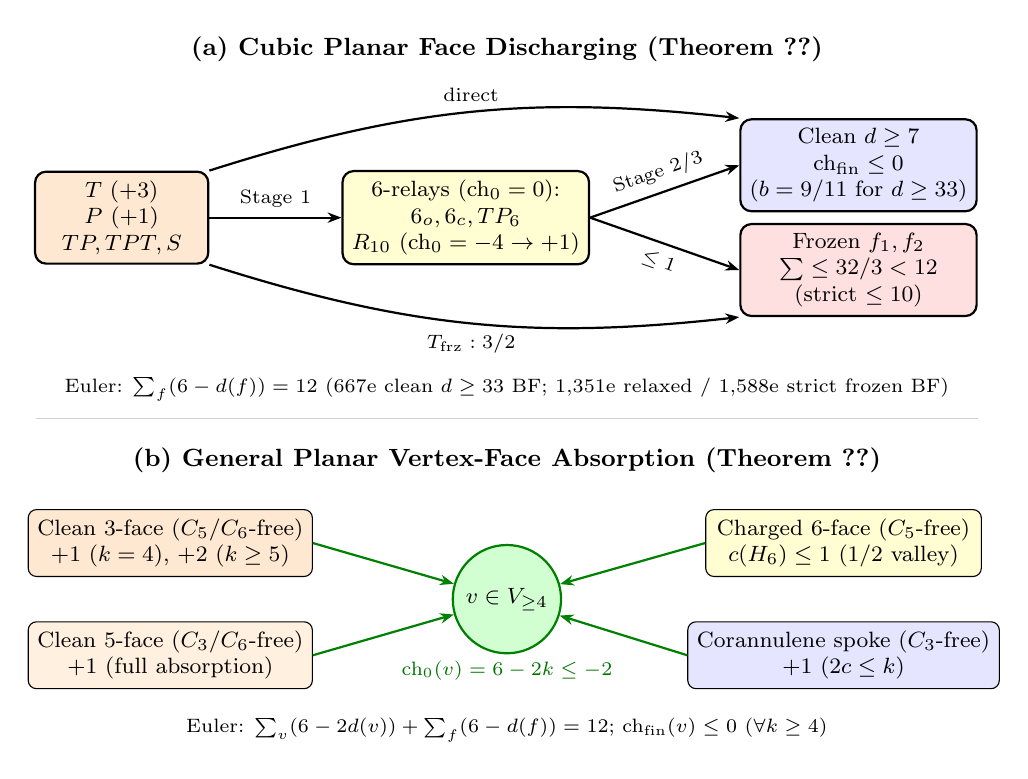
\begin{tikzpicture}[scale=0.95, every node/.style={font=\footnotesize}]
  % Top panel: Cubic Face Discharging
  \begin{scope}[shift={(0,5.25)}]
    \node[font=\bfseries\small] at (6.5, 4.10) {(a) Cubic Planar Face Discharging (Theorem~\ref{thm:main1})};
    \node[draw, rounded corners=4pt, fill=orange!18, thick, minimum width=2.2cm, align=center] (pos) at (1.35, 1.85) {$T\ (+3)$\\$P\ (+1)$\\$TP, TPT, S$};
    \node[draw, rounded corners=4pt, fill=yellow!18, thick, minimum width=3.1cm, align=center] (rel) at (5.95, 1.85) {$6$-relays ($\chz=0$):\\$6_o, 6_c, TP_6$\\$R_{10}$ ($\chz=-4\to+1$)};
    \node[draw, rounded corners=4pt, fill=blue!10, thick, minimum width=3.0cm, align=center] (cln) at (11.2, 2.55) {Clean $d \ge 7$\\$\chf \le 0$\\($b=9/11$ for $d\ge 33$)};
    \node[draw, rounded corners=4pt, fill=red!12, thick, minimum width=3.0cm, align=center] (frz) at (11.2, 1.15) {Frozen $f_1, f_2$\\$\sum \le 32/3 < 12$\\(strict $\le 10$)};

    \draw[-{Stealth[length=5pt]}, thick] (pos) -- node[above, font=\scriptsize]{Stage 1} (rel);
    \draw[-{Stealth[length=5pt]}, thick] (pos.north east) to[bend left=12] node[above, font=\scriptsize]{direct} (cln.north west);
    \draw[-{Stealth[length=5pt]}, thick] (pos.south east) to[bend right=12] node[below, font=\scriptsize]{$T_{\mathrm{frz}}: 3/2$} (frz.south west);
    \draw[-{Stealth[length=5pt]}, thick] (rel.east) -- node[above, sloped, font=\scriptsize]{Stage 2/3} (cln.west);
    \draw[-{Stealth[length=5pt]}, thick] (rel.east) -- node[below, sloped, font=\scriptsize]{$\le 1$} (frz.west);

    \node[align=center, font=\scriptsize] at (6.5, -0.45) {Euler: $\sum_f (6 - d(f)) = 12$ ($667$e clean $d\ge 33$ BF; $1{,}351$e relaxed / $1{,}588$e strict frozen BF)};
  \end{scope}

  \draw[gray!35] (0.2, 4.42) -- (12.8, 4.42);

  % Bottom panel: General Planar Vertex-Face Absorption
  \begin{scope}[shift={(0,0)}]
    \node[font=\bfseries\small] at (6.5, 3.85) {(b) General Planar Vertex-Face Absorption (Theorem~\ref{thm:main3})};
    \node[circle, draw=green!50!black, fill=green!18, thick, minimum size=1.05cm] (v) at (6.5, 2.0) {$v \in \Vge$};
    \node[font=\scriptsize, green!45!black, align=center] at (6.5, 1.05) {$\chz(v) = 6-2k \le -2$};

    \node[draw, rounded corners=3pt, fill=orange!18, minimum width=3.5cm, align=center] (t1) at (2.0, 2.75) {Clean $3$-face ($C_5/C_6$-free)\\$+1$ ($k=4$), $+2$ ($k\ge 5$)};
    \node[draw, rounded corners=3pt, fill=orange!12, minimum width=3.5cm, align=center] (p1) at (2.0, 1.25) {Clean $5$-face ($C_3/C_6$-free)\\$+1$ (full absorption)};
    \node[draw, rounded corners=3pt, fill=yellow!18, minimum width=3.5cm, align=center] (h1) at (11.0, 2.75) {Charged $6$-face ($C_5$-free)\\$c(H_6)\le 1$ ($1/2$ valley)};
    \node[draw, rounded corners=3pt, fill=blue!10, minimum width=3.5cm, align=center] (c1) at (11.0, 1.25) {Corannulene spoke ($C_3$-free)\\$+1$ ($2c \le k$)};

    \draw[-{Stealth[length=5pt]}, thick, green!50!black] (t1.east) -- (v);
    \draw[-{Stealth[length=5pt]}, thick, green!50!black] (p1.east) -- (v);
    \draw[-{Stealth[length=5pt]}, thick, green!50!black] (h1.west) -- (v);
    \draw[-{Stealth[length=5pt]}, thick, green!50!black] (c1.west) -- (v);

    \node[align=center, font=\scriptsize] at (6.5, 0.25) {Euler: $\sum_v (6-2d(v)) + \sum_f (6-d(f)) = 12$; $\chf(v) \le 0\ (\forall k \ge 4)$};
  \end{scope}
\end{tikzpicture}
\caption{Discharging architecture: (a)~three-stage cubic face discharging for Theorem~\ref{thm:main1} (distinguishing zero-initial-charge $6$-face relays from the Stage-2 $10$-face relay $R_{10}$ whose $-4$ deficit is filled to $+1$ by five triangles, and qualifying the $9/11$ slope for clean $d \ge 33$); (b)~general planar vertex-face absorption at independent high-degree sinks $v \in \Vge(H^+)$ for Theorem~\ref{thm:main3}, labeled by forbidden-cycle regime.}\label{fig:discharging}
\end{figure}

\subsection{Sharpness Witnesses: \texorpdfstring{$C_{60}$, $TD_{60}$, and $119$-Vertex $\Delta = 6$ $1$-Sums}{C60, TD60, and 119-Vertex Delta=6 1-Sums}}\label{subsec:trilogy-sharp}

The Lean~4 module \texttt{SharpWitnesses.lean} kernel-verifies that the truncated icosahedron $C_{60}$ ($60$ vertices, $90$ edges, $12$ pentagons $+$ $20$ hexagons) and truncated dodecahedron $TD_{60}$ ($60$ vertices, $90$ edges, $20$ triangles $+$ $12$ decagons) are nonempty cubic plane maps with exact dart bijections and single cyclic rotations at every vertex, explicit simple $C_{16}$ cycles, and no $C_3, C_4, C_8$ (for $C_{60}$) or no $C_4, C_5, C_6, C_7, C_8, C_9$ (for $TD_{60}$).

\begin{proposition}[$119$-Vertex $\Delta = 6$ Planar $1$-Sums]\label{prop:1sum}
For $H \in \{C_{60}, TD_{60}\}$, let $H \cdot H$ be the $1$-sum obtained by taking two disjoint copies $H^{(1)}, H^{(2)}$ of $H$ and identifying a single vertex $v_0^{(1)} \in V(H^{(1)})$ with a single vertex $v_0^{(2)} \in V(H^{(2)})$ into a cut-vertex $v_0$. Then $H \cdot H$ is a finite simple planar graph on $119$ vertices with $\delta(H \cdot H) = 3$, $\Delta(H \cdot H) = 6$, an explicit simple $C_{16}$, and the exact same forbidden-cycle exclusions as $H$ (no $C_3, C_4, C_8$ for $C_{60} \cdot C_{60}$; no $C_4,\dots,C_9$ for $TD_{60} \cdot TD_{60}$).
\end{proposition}

\begin{proof}
Fix a planar embedding of $H$ in a closed disk with $v_0$ on the outer boundary circle. Placing a copy of $H^{(1)}$ and a copy of $H^{(2)}$ in two disks tangent solely at $v_0$ produces a planar embedding of $H \cdot H$ on $S^2$. Clearly $|V(H \cdot H)| = 60 + 60 - 1 = 119$, $d(v_0) = 3 + 3 = 6$, and every other vertex retains degree $3$. Every simple cycle $C$ in $H \cdot H$ visits the cut-vertex $v_0$ at most once and therefore lies entirely within $H^{(1)}$ or entirely within $H^{(2)}$; hence the set of simple cycle lengths of $H \cdot H$ equals that of $H$.
\end{proof}

%% =============================================================================
\section{Main Theorem 4: Alternating-\texorpdfstring{$C_6$}{C6} Planar Degree-Density Bound}\label{sec:density}
%% =============================================================================

We give a completely self-contained graph-level proof of Theorem~\ref{thm:main4}, including the girth-$\ge 10$ Euler edge bound for arbitrary (possibly disconnected or acyclic) planar graphs.

\begin{lemma}[Planar Girth-$\ge 10$ Edge Bound with Bridges and Components]\label{lem:girth10-general}
Every finite simple planar graph $Q'$ on $n \ge 6$ vertices whose cycles all have length at least $10$ (allowing disconnected components, bridges, and tree components) satisfies
\begin{equation}\label{eq:girth10-bound}
  4 |E(Q')| \;\le\; 5(n - 2).
\end{equation}
\end{lemma}

\begin{proof}
Embed $Q'$ in $S^2$. If $Q'$ has $c \ge 2$ connected components, repeatedly add a bridge edge between two distinct components across a common face until a \emph{connected} simple planar graph $Q''$ on the same $n$ vertices is obtained; adding bridges creates zero cycles, so every cycle of $Q''$ still has length $\ge 10$, while $|E(Q')| \le |E(Q'')|$.

If $Q''$ is a tree, then $|E(Q'')| = n - 1$, and $4(n - 1) \le 5(n - 2) \iff n \ge 6$, establishing~\eqref{eq:girth10-bound}. Otherwise $Q''$ contains at least one cycle (of length $\ge 10$). Repeatedly delete any vertex of degree $1$ (leaf) from $Q''$; each deletion removes $1$ vertex and $1$ edge while preserving connectivity and girth $\ge 10$. Let $Q^*$ be the resulting connected simple planar graph on $n^* \le n$ vertices with $\delta(Q^*) \ge 2$, having deleted $t = n - n^* \ge 0$ leaves (so $|E(Q'')| = |E(Q^*)| + t$). Because $Q^*$ contains a cycle of length $\ge 10$, $n^* \ge 10$.

Consider any cellular spherical embedding of $Q^*$ and any facial boundary walk $W$ of a face $f$, and let $H_W \subseteq Q^*$ be the subgraph formed by the edges of $W$. We claim $H_W$ contains a cycle. Suppose to the contrary that $H_W$ is a tree; since $W$ is non-trivial, $H_W$ has a leaf $v$ ($\deg_{H_W}(v) = 1$) incident to a unique edge $e$ of $H_W$. Then both sides of $e$ belong to $f$, so the cyclic rotation at $v$ contains no other edge of $Q^*$ incident to $v$ (any other edge $e' \neq e$ at $v$ adjacent to $e$ in the rotation would necessarily lie on $\partial f$, forcing $e' \in E(H_W)$). Hence $\deg_{Q^*}(v) = 1$, contradicting $\delta(Q^*) \ge 2$. Therefore every facial walk $W$ traverses at least one cycle of $Q^*$ and hence has length $d(f) \ge |E(H_W)| \ge 10$.

Summing over all $|F^*|$ faces of $Q^*$ yields $10 |F^*| \le \sum_{f} d(f) = 2 |E(Q^*)|$. Substituting $|F^*| = 2 - n^* + |E(Q^*)|$ from Euler's formula~\eqref{eq:euler-general} gives $10(2 - n^* + |E(Q^*)|) \le 2|E(Q^*)|$, i.e., $8 |E(Q^*)| \le 10(n^* - 2)$, so $4 |E(Q^*)| \le 5(n^* - 2)$ (matching Lean~4 \texttt{planar\_girth10\_edge\_bound}). Adding back the $t$ deleted leaves gives
\[
  4 |E(Q')| \;\le\; 4 |E(Q'')| \;=\; 4 |E(Q^*)| + 4 t \;\le\; 5(n^* - 2) + 5 t \;=\; 5(n - 2). \qedhere
\]
\end{proof}

\begin{proof}[Proof of Theorem~\ref{thm:main4}]
First, we prove $n \ge 7$. Every vertex $v \in V(G)$ has $d_G(v) \ge 3$ and hence contributes $\binom{d_G(v)}{2} \ge \binom{3}{2} = 3$ unordered pairs of neighbors in $\binom{V(G)}{2}$. Because $G$ is $C_4$-free, no unordered pair $\{x, y\} \in \binom{V(G)}{2}$ can have two distinct common neighbors in $G$. Counting pairs yields
\[
  3 n \;\le\; \sum_{v \in V(G)} \binom{d_G(v)}{2} \;\le\; \binom{n}{2} \;=\; \frac{n(n - 1)}{2},
\]
which forces $n \ge 7$ since $n > 0$ (kernel-checked in \texttt{c4\_free\_min\_order}).

Next, let $Q := G[\Vge(G), V_3(G)]$ be the mixed bipartite spanning subgraph of $G$ consisting of all edges joining $\Vge(G)$ to $V_3(G)$. Because $\Vge(G)$ is an independent set, every edge incident to a vertex $v \in \Vge(G)$ lies in $Q$, so
\[
  |E(Q)| \;=\; \sum_{v \in \Vge(G)} d_G(v) \;=\; 4 h + \varepsilon.
\]
Let $T \subseteq E(Q)$ be a minimum-cardinality edge set intersecting every $6$-cycle of $Q$, so $|T| = \tau_6$, and set $Q' := Q - T$. Then $Q'$ is a planar bipartite graph on $n \ge 7 > 6$ vertices containing no odd cycles, no $C_4$ or $C_8$ (inherited from $G$), and no $C_6$ (by choice of $T$). Hence every cycle of $Q'$ has length at least $10$. Applying Lemma~\ref{lem:girth10-general} to $Q'$ gives $4|E(Q')| \le 5(n - 2)$. Since $4h + \varepsilon = |E(Q)| = |E(Q')| + \tau_6$, multiplying by $4$ gives
\[
  16 h + 4 \varepsilon \;=\; 4|E(Q')| + 4\tau_6 \;\le\; 5(n - 2) + 4\tau_6,
\]
proving~\eqref{eq:alt-c6-density} (Lean~4 \texttt{alternating\_c6\_density}).

For~(i), when $G$ is $C_6$-free we have $\tau_6 = 0$, so $16 h \le 16 h + 4\varepsilon \le 5(n - 2)$. Since $|V_3(G)| + h = n$ (as $\delta(G) \ge 3$),
\[
  16 |V_3(G)| \;=\; 16 n - 16 h \;\ge\; 16 n - 5(n - 2) \;=\; 11 n + 10.
\]
Thus $|V_3(G)| \ge \lceil(11n + 10)/16\rceil$, and since $3(11n + 10) = 33n + 30 > 32n$ for all $n \ge 1$, we have $|V_3(G)| > 2n/3$ with asymptotic slope gain $11/16 - 2/3 = 1/48$, establishing~\eqref{eq:v3-density} (Lean~4 \texttt{c6\_free\_v3\_density}).

For~(ii), if $|V_3(G)| \le 2n/3$, then $h = n - |V_3(G)| \ge n/3$, so~\eqref{eq:alt-c6-density} yields
\[
  4 \tau_6 \;\ge\; 16 \cdot \frac{n}{3} + 4 \varepsilon - 5(n - 2) \;=\; \frac{n + 30}{3} + 4 \varepsilon
  \;\implies\; \tau_6 \;\ge\; \left\lceil \frac{n + 30}{12} + \varepsilon \right\rceil.
\]
Finally, the edge union of any maximal collection of $m$ pairwise edge-disjoint $6$-cycles in $Q$ is a $6$-cycle edge transversal of size $6m \ge \tau_6$, giving $m \ge \lceil \tau_6 / 6 \rceil$.
\end{proof}

%% =============================================================================
\section{Formal Verification, Reproducibility, and Honest Scope}\label{sec:verification}
%% =============================================================================

All discrete algebraic/discharging components, proof-carrying dual potentials, $6{,}772$ strict-schema explicit simple dyadic-cycle patch entries (counted with multiplicity across cited certificate groups), and cellular-rotation sharpness certificates are formalized in pure Lean~4 (\texttt{v4.36.0}, commit \texttt{611c117b}, \texttt{import Std}, zero Mathlib) inside \texttt{paper1\_planar/lean/} at \url{https://github.com/lollipoll/erdos-gyarfas}. A full single-threaded build (\texttt{LEAN\_NUM\_THREADS=1 lake build}, $64$ jobs) compiles with exit code $0$ and zero warnings (cold baseline $1{,}035\,\mathrm{s}$, peak RSS $1.37\,\mathrm{GiB}$), and \texttt{lake env lean AxiomCheck.lean} confirms that all $106$ audited declarations use only $\{\texttt{propext}, \texttt{Classical.choice}, \texttt{Quot.sound}\}$ with zero \texttt{sorry}, zero custom axioms, and zero \texttt{native\_decide}.

In parallel, two pure-stdlib zero-float Python~3 verifiers (both AST-guarded against floats and true division~\texttt{/}) validate the finite searches and Lean--Python--JSON alignment:
\begin{enumerate}[label=(\alph*),leftmargin=2.2em]
  \item \texttt{cert/verify\_planar\_eg.py} replays all underlying finite searches, boundary-weld and outer-rim enumerations, conservative $d \in \{14,17,18\}$ enumerations, uncollapsed cyclic DPs, Bellman--Ford potentials, and $119$-vertex $1$-sum witnesses in ${\sim}21\,\mathrm{s}$ (peak RSS $43\,\mathrm{MiB}$), reproducing all four deterministic JSON witness tables in \texttt{cert/witnesses/} byte for byte;
  \item \texttt{cert/verify\_parity\_and\_dp.py} directly verifies literal parity across Lean~4 data modules, \texttt{cert/witnesses/*.json}, and live replay of \texttt{verify\_planar\_eg.py} across all $6{,}772$ weld/rim entries, confirms the Lemma~\ref{lem:weld-sound} boundary-regularity invariant across all $844/844$ production \texttt{enum\_planar\_welds} calls, checks all $12$ weighted forward-simulation proofs linking the uncollapsed $C_5$-free ($7$ degrees: $d \in \{9..14, 17\}$) and $C_6$-free ($5$ degrees: $d \in \{9, 11..14\}$) DPs to the packed Lean automata, and replays all supplemental manuscript subaudits (cubic \texttt{Triad-D1} $4$-edge seals, $d = 9$ flag welds, $d = 17$ $6_o$ $112$-case contact test, $d \in \{14, 18\}$ $6_o$ $1$-drop replay, $d = 17$ $TP_{s3}$ $(0..3)$ post-sieve $496$-residual check, and all $14{,}962$ $C_5$-free Stage-3 outer-rim capacity kills) in ${\sim}43\,\mathrm{s}$ (peak RSS $70\,\mathrm{MiB}$).
\end{enumerate}
Table~\ref{tab:traceability} summarizes the exact honest boundary between Lean~4 kernel proofs, finite proof-carrying certificates/Python replay, and manuscript proofs.

\begin{table}[t]
\centering
\caption{Honest Lean-to-Theorem Traceability Matrix separating kernel-verified Lean~4 components, finite certificates/Python replay, and manuscript proofs.}\label{tab:traceability}
\scriptsize
\setlength{\tabcolsep}{4pt}
\begin{tabular}{@{}>{\raggedright\arraybackslash}p{2.1cm}>{\raggedright\arraybackslash}p{4.6cm}>{\raggedright\arraybackslash}p{4.6cm}>{\raggedright\arraybackslash}p{4.2cm}@{}}
\toprule
\textbf{Paper Claim} & \textbf{Proved in Lean~4 Kernel} & \textbf{Proof-Carrying / Python Replay} & \textbf{Proved in Manuscript} \\
\midrule
Shared Euler \& Caps (Sec.~\ref{sec:prelim}) &
\texttt{FinGraph}, \texttt{PlaneMap}, \texttt{euler\_face\_discharging\_sum}, \texttt{euler\_vertex\_face\_sum}, \texttt{charge\_conservation\_contradiction}, \texttt{minimal\_two\_edge\_bond\_cap\_deg}, \texttt{universal\_two\_vertex\_cut\_cap\_min\_deg}, \texttt{cap\_cycle\_avoiding\_edge\_lifts} &
Deterministic verifier self-tests (\texttt{verify\_engine\_self\_tests}) on hereditary vs.\ emit-only welding and disconnected subcubic cycle search &
Spherical rotation systems, Euler $V-E+F=1+c$, Whitney simple dual (Lem.~\ref{lem:plane-basics}), Minimal $2$-Edge-Bond Cap (Lem.~\ref{lem:cubic-cap}), Universal $2$-Vertex-Cut Cap \& $\Vge$-independence (Lem.~\ref{lem:general-cap}) \\
\addlinespace
Thm.~\ref{thm:main1}: Cubic Planar $C_{32}$ (Sec.~\ref{sec:cubic}) &
\texttt{main\_theorem\_1\_cubic\_planar\_c32} (component/certificate assembly), \texttt{cubic\_relaxed\_discharging\_contradiction}, BF/DP/BWD soundness, \texttt{weldSchema\_valid\_of\_bool}, \texttt{weldFaceGraph\_hasDyadicCycle}, $G_{168}$ cubic/$3$-conn./dart bijection/single rotation/no $C_4,C_8,C_{16}$/$C_{32}$ &
Packed BF ($667$e $d\ge 33$, $1{,}351$e relaxed core, $1{,}588$e strict frozen), clean $d\le 31$ DP/BWD, $51$ chains ($1{,}581$ tested / $1{,}327$ pruned welds), $520$ seal welds, $108$ $d=17$ residuals ($48$ words $\to 114$ welds $+ 5$ reused $R_{10}$ seals); all $1{,}966$ entries strict-schema + simple $C_4..C_{32}$; $844/844$ weld invariant \& supplemental \texttt{Triad-D1}/$d=9$/$6_o$/$TP_{s3}$ subaudits replayed in \texttt{verify\_parity\_and\_dp.py} &
Boundary-weld dart-parity, Euler \& lifting (Lem.~\ref{lem:weld-sound}), deterministic cubic discharging rules (Sec.~\ref{subsec:cubic-rules}), complete \texttt{pair\_ok}/flags/CAP maps, exact \texttt{starts\_N} \& conservative shift/splice soundness (Lem.~\ref{lem:startsN}) \\
\addlinespace
Thm.~\ref{thm:main2}: Planar Claw-Free $C_{64}$ (Sec.~\ref{sec:clawfree}) &
\texttt{main\_theorem\_2\_planar\_clawfree\_c64} (component/certificate assembly: arithmetic/forest assembly coupled to cubic packed BF), \texttt{bowtie\_forest\_exclusion}, \texttt{forest\_edge\_bound\_on\_cycle}, \texttt{universal\_bowtie\_transfer}, \texttt{dyadic\_cycle\_lift\_window} &
Bounded Python arithmetic verification across $L \le 500$ ($r \in \{0,1,2\}$ and lift endpoints) &
Induced claw-free $C_4$-free representation $G \cong T(H)/B$, Planar Bowtie-Splitting (Lem.~\ref{lem:clawfree-split}), simple cycle realization across $[2L-k, 3L-k-m]$, local forest lift (Lem.~\ref{lem:lift-window}) \\
\addlinespace
Thm.~\ref{thm:main3}: General Planar $C_{16}$ Trilogy (Sec.~\ref{sec:trilogy}) &
\texttt{main\_theorem\_3\_general\_planar\_c16\_trilogy} (component/certificate assembly), \texttt{general\_planar\_discharging\_contradiction}, \texttt{c3free\_vertex\_absorption}, \texttt{c6free\_vertex\_absorption}, \texttt{c5free\_f10\_5tri\_bound} ($47/12<4$), $C_{60}$/$TD_{60}$ dart bijection/single rotation/cycles &
Packed $C_3/C_5/C_6$ BF \& DP ($12/12$ weighted collapse simulations verified in \texttt{verify\_parity\_and\_dp.py}), all $4{,}806$ ($1{,}260+3{,}501+45$) strict-schema + simple $C_4/C_8/C_{16}$ rim kills, $14{,}962$ supplemental $C_5$-free Stage-3 rim kills replayed in \texttt{verify\_parity\_and\_dp.py}, $119$-v $1$-sum verifier checks &
Edge-minimality $\Vge$-independence, exterior-disk noncrossing rim-quotient soundness \& seed completeness (Lem.~\ref{lem:rim-sound}), complete $C_3/C_5/C_6$ discharging rules, $25$-seed valley-$9$ \& $9$-seed $C_6$ reductions, $119$-v $\Delta=6$ $1$-sum gluing (Prop.~\ref{prop:1sum}) \\
\addlinespace
Thm.~\ref{thm:main4}: Alt.-$C_6$ Density (Sec.~\ref{sec:density}) &
\texttt{main\_theorem\_4\_alternating\_c6\_density} (component/certificate assembly: girth-$10$/order/density algebra), \texttt{planar\_girth10\_edge\_bound}, \texttt{alternating\_c6\_density}, \texttt{c4\_free\_min\_order}, \texttt{c6\_free\_v3\_density}, $+1/48$ identity &
Python arithmetic checks for $n < 500$ and $\tau_6$ lower bounds &
Mixed bipartite $Q$, transversal deletion $Q \to Q'$, girth-$\ge 10$ Euler bound allowing bridges/components/forests (Lem.~\ref{lem:girth10-general}), $3n \le \binom{n}{2}$ pair bound \\
\bottomrule
\end{tabular}
\end{table}

\section*{Declaration of Generative AI and AI-Assisted Technologies in the Manuscript Preparation Process}

During the preparation of this work, the author used \emph{Gemini 4 Neon} to assist with interactive proof exploration, discharging-rule and certificate design, Lean~4 formalization, and manuscript drafting, and used \emph{GPT 6.2 Astra} to perform an AI-assisted adversarial audit of the author's Lean~4 declarations, Python verification scripts, certificate parity, and manuscript proofs. Machine verification is separated strictly across four layers rather than relying on unverified model output: core discrete algebraic/discharging components and packed certificate bounds are kernel-checked in Lean~4 (\texttt{v4.36.0}), underlying finite searches and uncollapsed dynamic programs are replayed by \texttt{cert/verify\_planar\_eg.py}, literal Lean--Python--JSON parity and the $12$ weighted state-collapse simulations are checked by \texttt{cert/verify\_parity\_and\_dp.py}, and all topological and graph-theoretic reductions are proved in this manuscript. After using these tools, the author reviewed, edited, and verified the content as needed and takes full responsibility for the content of the publication, including all mathematical claims, proofs, code, and references.

\begin{thebibliography}{99}

\bibitem{Carr2026}
A.~Carr,
\emph{Every minimal counterexample to the Erd\H{o}s--Gy\'arf\'as conjecture is predominantly cubic},
arXiv:2605.22844 (2026).

\bibitem{DanielShauger2001}
D.~Daniel and S.~E.~Shauger,
\emph{A result on the Erd\H{o}s--Gy\'arf\'as conjecture in planar graphs},
Congressus Numerantium \textbf{153} (2001), 129--139.

\bibitem{DucoffeDumitru2026}
G.~Ducoffe and B.~Dumitru,
\emph{Towards a more structured search for Erd\H{o}s--Gy\'arf\'as counter-examples},
arXiv:2609.28594 (2026).

\bibitem{Erdos1997}
P.~Erd\H{o}s,
\emph{Some old and new problems in various branches of combinatorics},
Discrete Mathematics \textbf{165/166} (1997), 227--231.

\bibitem{Exoo2014}
G.~Exoo,
\emph{Three graphs and the Erd\H{o}s--Gy\'arf\'as conjecture},
arXiv:1403.5636 (2014).

\bibitem{Garcia2026}
D.~Garcia,
\emph{Small graphs without power-of-two cycles: a lower bound of $24$, a correction to a construction of Exoo, and explicit bounds for $f(k)$},
arXiv:2609.04686 (2026).

\bibitem{HeckmanKrakovski2013}
C.~C.~Heckman and R.~Krakovski,
\emph{Erd\H{o}s--Gy\'arf\'as conjecture for cubic planar graphs},
Electronic Journal of Combinatorics \textbf{20}(2) (2013), \#P7.

\bibitem{LiuMontgomery2023}
H.~Liu and R.~Montgomery,
\emph{A solution to Erd\H{o}s and Hajnal's odd cycle problem},
Journal of the American Mathematical Society \textbf{36}(4) (2023), 1191--1234.

\bibitem{Markstrom2004}
K.~Markstr\"om,
\emph{Extremal graphs for some problems on cycles in graphs},
Congressus Numerantium \textbf{171} (2004), 179--192.

\bibitem{Shauger1998}
S.~E.~Shauger,
\emph{Results on the Erd\H{o}s--Gy\'arf\'as conjecture in $K_{1,m}$-free graphs},
Congressus Numerantium \textbf{134} (1998), 61--65.

\bibitem{SudakovVerstraete2008}
B.~Sudakov and J.~Verstra\"ete,
\emph{Cycle lengths in sparse graphs},
Combinatorica \textbf{28}(3) (2008), 357--372.

\end{thebibliography}

\end{document}
